
\documentclass[a4paper, 11pt, titlepage]{scrbook}
\usepackage[utf8]{inputenc}
\usepackage[spanish]{babel}
% \usepackage[T1]{fontenc}  
% \usepackage{lmodern}


\usepackage{todonotes}

\usepackage{csquotes}
\usepackage{epigraph}
\usepackage[backend=biber, style=apa]{biblatex}
\setcounter{biburllcpenalty}{7000}
\setcounter{biburlucpenalty}{8000}
\addbibresource{bibliografia/bibliografia.bib}
\DeclareFieldFormat[online]{citetitle}{#1}
\DeclareFieldFormat[online]{title}{#1} 



\usepackage{fancyhdr}
\usepackage{graphicx}
\usepackage{hyperref} %referencia
\usepackage{booktabs}
\usepackage{tabularx}
\usepackage{geometry}
\usepackage{expex} % para glosas


\usepackage{pdfpages}

\usepackage[acronym]{glossaries}
\makenoidxglossaries
% Lista de acrónimos 
% Para llamarlos usar \acrshort
\newacronym{aes}{AES}{Advanced Encryption Standard}
\newacronym{api}{API}{Application Programming Interface}
\newacronym{captcha}{CAPTCHA}{Completely Automated Public Turing test to tell Computers and Humans Apart}
\newacronym{cbc}{CBC}{Cipher Block Chaining}
\newacronym{cicd}{CI/CD}{Continuous Integration / Continuous Delivery}
\newacronym{cpu}{CPU}{Central Processing Unit}
\newacronym{crud}{CRUD}{Create, Read, Update, Delete}
\newacronym{csrf}{CSRF}{Cross-Site Request Forgery}
\newacronym{css}{CSS}{Cascading Style Sheets}
\newacronym{db}{DB}{Database}
\newacronym{vdom}{VDOM}{Virtual Document Object Model}
\newacronym{ecb}{ECB}{Electronic Codebook}
\newacronym{ecc}{ECC}{Elliptic Curve Cryptography}
\newacronym{javaee}{Java EE}{Java Enterprise Edition}
\newacronym{gb}{GB}{Gigabyte}
\newacronym{gcm}{GCM}{Galois/Counter Mode}
\newacronym{get}{GET}{Hypertext Transfer Protocol GET Method}
\newacronym{html}{HTML}{HyperText Markup Language}
\newacronym{http}{HTTP}{HyperText Transfer Protocol}
\newacronym{ide}{IDE}{Integrated Development Environment}
\newacronym{idea}{IDEA}{International Data Encryption Algorithm}
\newacronym{jdk}{JDK}{Java Development Kit}
\newacronym{jpa}{JPA}{Java Persistence API}
\newacronym{jpql}{JPQL}{Java Persistence Query Language}
\newacronym{json}{JSON}{JavaScript Object Notation}
\newacronym{jsx}{JSX}{JavaScript XML}
\newacronym{mvc}{MVC}{Model-View-Controller}
\newacronym{post}{POST}{Hypertext Transfer Protocol POST Method}
\newacronym{put}{PUT}{Hypertext Transfer Protocol PUT Method}
\newacronym{ram}{RAM}{Random Access Memory}
\newacronym{rest}{REST}{Representational State Transfer}
\newacronym{rsa}{RSA}{Rivest–Shamir–Adleman (Cryptosystem)}
\newacronym{sid}{SID}{Sistema de Impresión de Documentos}
\newacronym{smtp}{SMTP}{Simple Mail Transfer Protocol}
\newacronym{spa}{SPA}{Single Page Application}
\newacronym{sql}{SQL}{Structured Query Language}
\newacronym{tls}{TLS}{Transport Layer Security}
\newacronym{uml}{UML}{Unified Modeling Language}
\newacronym{url}{URL}{Uniform Resource Locator}
\newacronym{xml}{XML}{eXtensible Markup Language}


\newglossaryentry{policies}{
    name=policies,
    description={son las reglas y modelos que determinan cómo el asistente virtual decide cuál será la próxima acción en una conversación, basándose en el contexto y el historial del diálogo.}
}

\newglossaryentry{pipeline}{
    name=pipeline,
    description={secuencia de componentes y pasos configurados para procesar datos, extraer características, y entrenar modelos que permiten al asistente virtual comprender e interpretar el lenguaje natural. En caso de Rasa se encuentra en config.yaml}
}

\newglossaryentry{metodologia agil}{
    name=metodología ágil,
    description={
        En el desarrollo de software, las prácticas ágiles consisten en la mejora de requisitos, investigación y soluciones mediante el esfuerzo colaborativo de equipos autoorganizados y multifuncionales junto con sus clientes/usuarios finales.
    }
}





% CODIGO
\usepackage{listings}
\lstset{
    basicstyle=\ttfamily\small,
    breaklines=true, % Permite el salto de línea automático
    frame=single, % Añade un marco alrededor del código
    backgroundcolor=\color{gray!10}, % Fondo gris claro
    keywordstyle=\color{blue}, % Palabras clave en azul
    commentstyle=\color{green!50!black}, % Comentarios en verde
    stringstyle=\color{red}, % Cadenas de texto en rojo
    showstringspaces=false, % No mostrar espacios en cadenas
    numbers=left, % Números de línea a la izquierda
    numberstyle=\tiny\color{gray}, % Estilo de los números de línea
    inputencoding=utf8,
    extendedchars=true,
    literate={á}{{\'a}}1 {ã}{{\~a}}1 {é}{{\'e}}1 {ó}{{\'o}}1 {ñ}{{\~n}}1 
}



% minimizar fragmentado de listados
\lstnewenvironment{listing}[1][]
   {\lstset{#1}\pagebreak[0]}{\pagebreak[0]}




\newcommand{\myTitle}{Digitalización, estructuración y preservación lingüística de gramáticas mayas minorizadas mediante inteligencia artificial multimodal}
\newcommand{\mySubtitle}{Automatización de la preservación de lenguas minorizadas: un enfoque basado en modelos de lenguaje y marcado XML}
\newcommand{\myDegree}{Máster en Inteligencia Artificial}
\newcommand{\myName}{Elías Alfonso Carrasco Guerrero}
\newcommand{\myProf}{Juan Antonio Pérez Ortiz}
\newcommand{\myFaculty}{Escuela Politécnica Superior de la Universidad de Alicante}
\newcommand{\myFacultyShort}{EPS UA}
\newcommand{\depTutorOne}{Departamento de Lenguajes y Sistemas Informáticos}


\newcommand{\myUni}{\protect{Universidad de Alicante}}
\newcommand{\myLocation}{Alicante}
\newcommand{\myTime}{\today}
\newcommand{\logoGrado}{imagenes/UA/logoim.jpg}
\newcommand{\logoFacultad}{imagenes/UA/logoeps.jpg}
\newcommand{\logoUniversidad}{imagenes/UA/logoua.jpg}

\usepackage{url}


\pagestyle{fancy}
\fancyhf{}
\fancyhead[LO]{\nouppercase\leftmark}
\fancyhead[RE]{\nouppercase\rightmark}
\fancyhead[RO,LE]{\thepage}


% \setlength{\headheight}{1.5\headheight}


% Para que en las páginas en blanco no ponga cabeceras
\makeatletter
\def\clearpage{%
  \ifvmode
    \ifnum \@dbltopnum =\m@ne
      \ifdim \pagetotal <\topskip
        \hbox{}
      \fi
    \fi
  \fi
  \newpage
  \thispagestyle{empty}
  \write\m@ne{}
  \vbox{}
  \penalty -\@Mi
}
\makeatother






\AtBeginDocument{%
  \renewcommand\tablename{Tabla}
  \renewcommand{\listtablename}{Índice de tablas} 
}


\renewcommand{\lstlistingname}{Listado}
\renewcommand{\lstlistlistingname}
             {Índice de \lstlistingname s}

\begin{document}
% portada
\frontmatter
\input{portada/portada} %la portada en color
\input{portada/portada_2} %la portada en b/n
\chapter{Resumen}

La aplicación desarrollada para este Trabajo de Fin de Máster consiste en un software modular programado en Python que se ejecuta desde la terminal de comandos. Su función principal es automatizar la extracción de texto y la comprensión visual de páginas en formato PDF pertenecientes a gramáticas de lenguas mayas. El sistema inyecta ejemplos estructurados de entrada y salida (few-shot) junto a un prompt especializado directamente en la memoria de la API de Gemini, logrando que el modelo de Inteligencia Artificial entienda la disposición tipográfica original y devuelva la información totalmente organizada en un archivo XML con etiquetas semánticas personalizadas (como <morpheme\_analysis> o <syntactic\_analysis>). Posteriormente, el pipeline procesa este archivo XML para generar de forma automática un documento en LaTeX que se compila para reconstruir la obra original en un nuevo archivo PDF con un acabado editorial profesional. El objetivo último es transformar "papel digital" estático en un conjunto de datos estructurados de alta precisión (Gold Standard) que sirva como combustible indispensable para que, en el futuro, otras Inteligencias Artificiales puedan entrenarse y aprender idiomas minorizados de bajos recursos computacionales.
Este Trabajo de Fin de Máster aborda la problemática de la digitalización y estructuración de gramáticas normativas de lenguas mayas minorizadas (Kaqchikel, K’iche’, Mam y Q’anjob’al), cuyos documentos originales presentan estructuras tipográficas complejas que dificultan el procesamiento mediante técnicas de OCR convencionales. Se propone y desarrolla un sistema automatizado basado en Modelos de Lenguaje de Gran Tamaño (LLMs) a través de la API de Gemini, integrado en un pipeline modular desarrollado en Python. Con este flujo se consigue mitigar la pérdida de información semántica y espacial inherente a los métodos planos tradicionales, salvaguardando recursos científicos de alto valor como las glosas interlineales.
La metodología se fundamenta en la transformación de documentos PDF en datos estructurados bajo el estándar XML, garantizando la integridad jerárquica mediante la definición de un Documento de Definición de Tipo (DTD) y el desarrollo de módulos específicos de corrección estructural (xml\_corrector.py). El núcleo de la investigación se centra en un estudio empírico sobre el parámetro de temperatura del modelo, evaluando su impacto en la precisión y estabilidad del sistema bajo una estricta "economía de tokens" impuesta por las limitaciones de cuota del entorno operativo.
Los resultados experimentales demuestran la existencia de un "punto dulce" (sweet spot) en temperaturas de 0.1 y 0.25, donde se alcanzan precisiones superiores al 90% incluso en casos de alta complejidad estructural y estrés informativo. Finalmente, el sistema automatiza la generación de documentación científica en LaTeX, permitiendo una reconstrucción fiel y profesional de los textos originales. El trabajo concluye que el uso de LLMs, correctamente parametrizados y validados mediante un entorno de control heurístico y formal, constituye una herramienta de alto valor para la preservación del patrimonio lingüístico digital y la soberanía tecnológica de las comunidades desfavorecidas.


\textbf{Palabras clave:} Inteligencia Artificial, LLM, Gemini API, Lenguas Mayas, Digitalización, XML, Procesamiento de Lenguaje Natural, OCR Estructurado.


\chapter*{Motivación y justificación}
\thispagestyle{empty}

La preservación de la diversidad lingüística constituye uno de los desafíos más críticos en la era de la información. Las lenguas minorizadas, en particular aquellas pertenecientes a la familia maya como el Kaqchikel, el K’iche’, el Mam y el Q’anjob’al, representan un patrimonio cultural de valor incalculable. Sin embargo, su supervivencia no sólo depende de su uso oral, sino también de la disponibilidad y accesibilidad de recursos académicos y normativos en formatos digitales modernos.
En este contexto, la Academia de Lenguas Mayas de Guatemala (ALMG) desempeña un papel crucial como entidad rectora en la promoción y estandarización de estos idiomas. A través de su repositorio institucional de documentos (disponible en https://almg.org.gt/documentos/), la ALMG ha realizado un esfuerzo significativo por poner a disposición del público gramáticas normativas y textos de referencia, tal y como se muestra en la figura \ref{fig:web_ALMG}. No obstante, gran parte de este conocimiento se encuentra consignado en archivos PDF que, si bien facilitan la difusión, actúan esencialmente como "papel digital": una representación estática de la información que carece de estructura semántica.


\begin{figure}
    \centering
    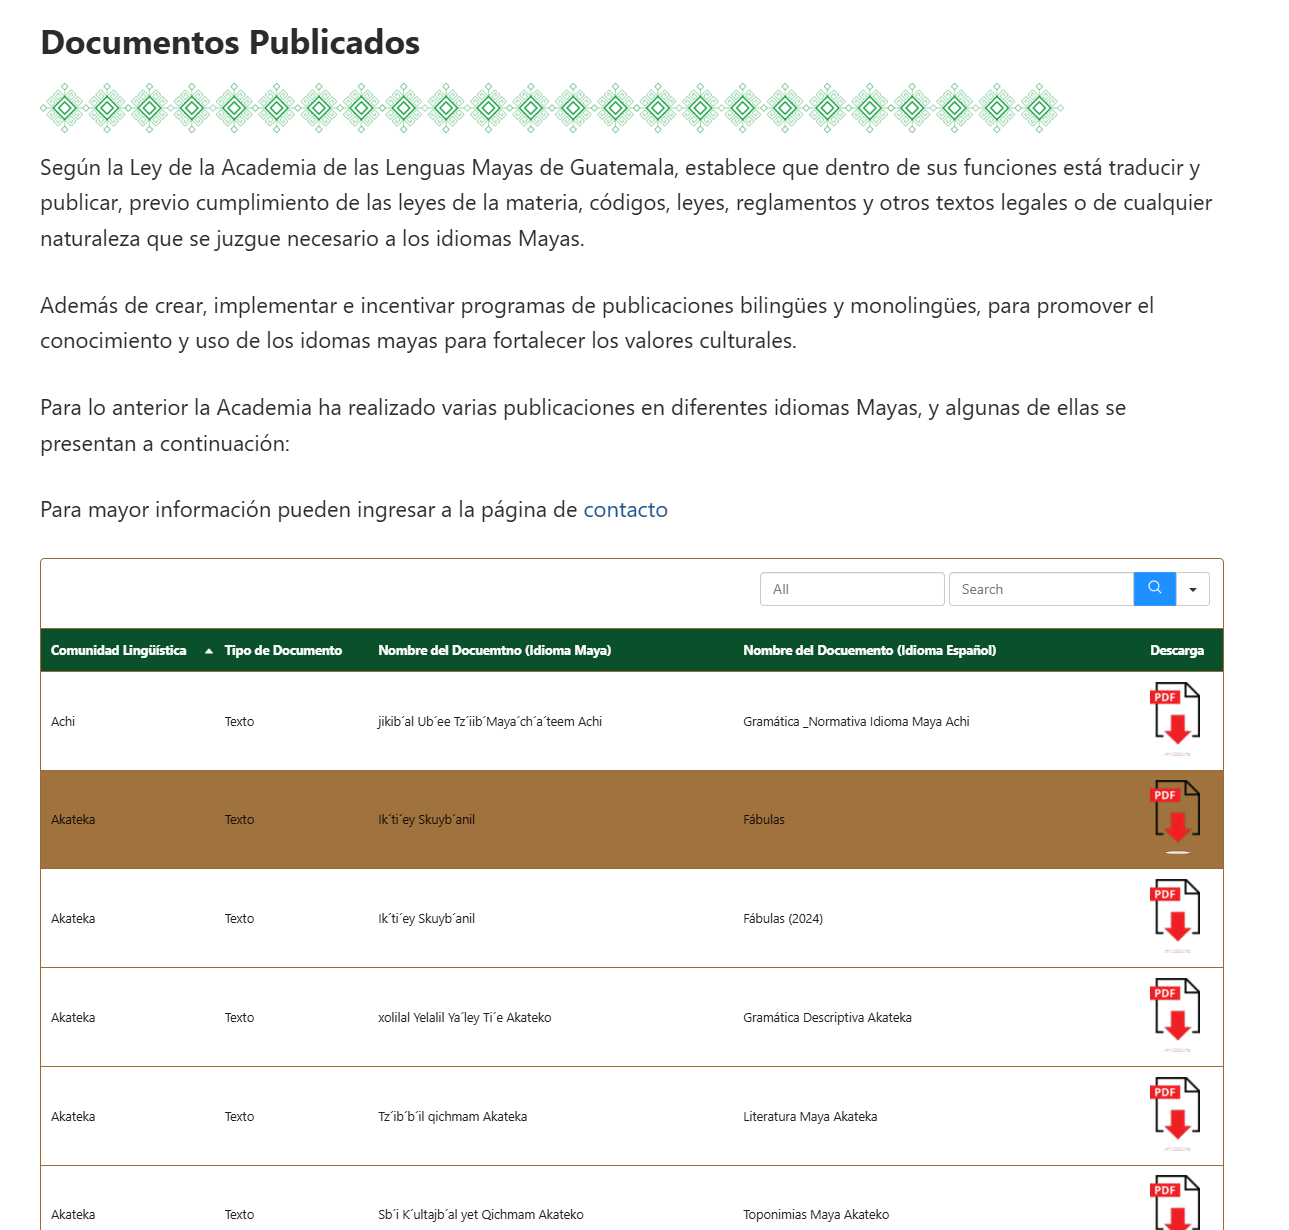
\includegraphics[width=0.95\linewidth]{imagenes/ALMG/web_ALMG.png}
    \caption{Web de la ALMG}
    \label{fig:web_ALMG}
\end{figure}

Por ejemplo, ya en marzo de 2025, tuvieron una actualización de la web en la que eliminaron el 70% de los documentos que tenían alojados, pasando de 200 a 60.
Esta limitación impide que los datos lingüísticos (ejemplos gramaticales, reglas sintácticas, morfología) puedan ser procesados automáticamente por herramientas computacionales, buscadores especializados o sistemas de aprendizaje profundo. La motivación técnica de este trabajo radica, por tanto, en la superación de las barreras impuestas por el reconocimiento óptico de caracteres (OCR) convencional sobre este corpus específico de la ALMG, para generar corpus con morfologías clasificadas para entrenamiento de modelos.
Las gramáticas lingüísticas de estas lenguas presentan una complejidad tipográfica elevada, que incluye tablas anidadas, glosas interlineales y estructuras jerárquicas que los sistemas tradicionales suelen interpretar de manera errónea. Ante este escenario, surge la oportunidad de emplear Modelos de Lenguaje de Gran Tamaño (LLMs), para comprender la arquitectura lógica de estos documentos institucionales y transformarla en datos estructurados bajo el estándar XML.
Este proyecto busca proporcionar una solución eficiente que reduzca la carga de trabajo manual en la digitalización del patrimonio de la ALMG, garantizando que la información sea interoperable, consultable y apta para la generación de documentación científica profesional mediante LaTeX.




\cleardoublepage %salta a nueva página impar
% Aquí va la dedicatoria si la hubiese. Si no, comentar la(s) linea(s) siguientes
\chapter*{Agradecimientos}
\setlength{\leftmargin}{0.5\textwidth}
\setlength{\parsep}{0cm}
\addtolength{\topsep}{0.5cm}

\begin{flushright}
\small\em{
A mi familia por estar ahí en todo momento.\\
A mi pareja por ayudarme en todo lo que puede y más.\\
A mi madre por dedicar su vida a sus hijos.\\
A mi padre por animarme con mi carrera en la ciencia.\\
A mis compañeros del Santander por guiarme y enseñarme cómo desarrollar software. \\
Sin ellos no habría podido hacer este trabajo.
}
\end{flushright}



\cleardoublepage %salta a nueva página impar
% Aquí va la cita célebre si la hubiese. Si no, comentar la(s) linea(s) siguientes
\chapter*{}
%\setlength{\leftmargin}{0.5\textwidth}
%\setlength{\parsep}{0cm}
%\addtolength{\topsep}{0.5cm}
\epigraph{
Pues hemos nacido para colaborar,
al igual que los pies, las manos,
los párpados, las hileras de dientes,
superiores e inferiores. 
Obrar, pues, como adversarios los unos de los otros
es contrario a la naturaleza.
}
{Marco Aurelio (Meditaciones)}
\vspace{4cm}
\epigraph{
    Solo los que se quemaron con el fuego aprendieron a usarlo.
}
{Andrés Pedreño Muñoz\\Cofundador de Torre Juana OST}

\cleardoublepage %salta a nueva página impar

%Con los siguientes comandos se genera el índice, indice de figuras, tablas y listados de código
\tableofcontents
\listoffigures
\listoftables
\lstlistoflistings

\mainmatter
\chapter{Introducción}
En la actualidad, la gestión eficiente de la información y la documentación es una necesidad crítica para muchas organizaciones. Empresas, instituciones y proyectos a gran escala dependen de bases de datos robustas para almacenar, organizar y acceder rápidamente a grandes volúmenes de documentos.

Sin embargo, uno de los desafíos más comunes es asegurarse de que los documentos estén correctamente almacenados, organizados y accesibles únicamente por el personal autorizado. Por ejemplo, el equipo de tecnologías de la información no debería tener acceso a la información contenida en un contrato de crédito.

A esto se suma que, en muchas empresas, la generación de documentos se delega a proveedores externos, lo que implica que el flujo de un documento pase por varias etapas. Esto aumenta el riesgo de que se produzcan pérdidas o errores en el almacenamiento. En este contexto, es crucial contar con herramientas que permitan realizar verificaciones automáticas y comprobar que los documentos se encuentran correctamente guardados.

Otro aspecto relevante es la necesidad de proteger la información confidencial. Para evitar comprometer la seguridad de los datos de clientes y empresas, es indispensable que las herramientas puedan verificar el correcto almacenamiento de los documentos sin acceder a su contenido o metadatos. Esta capacidad es fundamental para mantener la integridad y confidencialidad de la información.

El desarrollo de aplicaciones web con tecnologías modernas como Spring Boot, JPA y Thymeleaf ha cobrado gran relevancia debido a su capacidad para ofrecer soluciones eficientes en la gestión de bases de datos y el procesamiento de información. Estas tecnologías permiten crear aplicaciones ágiles y seguras, que pueden realizar operaciones complejas de filtrado, validación y acceso a datos en tiempo real.

La aplicación web propuesta en este proyecto tiene como objetivo facilitar el filtrado y la validación de documentos almacenados. Con este fin, se desarrollará una interfaz con una tabla que muestre campos del documento como su identificador y la hora a la que se almacenó en la base de datos, asegurando así su correcto almacenamiento y la consistencia de los datos, sin poder acceder a campos del documento con información confidencial.

Todo el código de la aplicación SIDManager está disponible en la plataforma GitHub de manera pública en el enlace a pie de página \footnote{\url{https://github.com/eliascarrasco1227/SIDManager}}. La aplicación sigue las indicaciones de la estrategia de software de código abierto (open source) de la Comisión Europea, como se puede ver en el enlace en el pie de página \footnote{\url{https://commission.europa.eu/about/departments-and-executive-agencies/digital-services/open-source-software-strategy_en\#opensourcesoftwarestrategy}}.

El nombre de esta aplicación, SIDManager, proviene de dos componentes.
El primero, \acrshort{sid}, corresponde con las siglas de \acrlong{sid}, un conjunto de scripts y aplicaciones web que se encargan de la gestión, impresión, envío y modificación de documentos.
El segundo componente, Manager, proviene del inglés y significa administrador, ya que es la web encargada de la administración de los documentos; es decir, sirve para verificar la situación de los documentos y ver si se han almacenado correctamente en la base de datos.

Finalmente, esta herramienta está diseñada para simplificar el acceso y la gestión de datos en entornos empresariales, priorizando la seguridad, el rendimiento y la escalabilidad. Al mismo tiempo, desacopla la lógica de negocio de la aplicación, ya que no necesita acceder al contenido de los documentos. 

Con la implementación de Spring Security, se garantiza un acceso seguro, mientras que log4j permite un seguimiento detallado de las operaciones y posibles incidencias. De este modo, el proyecto ofrece una solución accesible y eficiente para cualquier empresa o individuo que necesite verificar y gestionar documentos, sin recurrir a equipos especializados o productos de software externos.

%\chapter{Estudio de viabilidad}

El desarrollo de cualquier proyecto tecnológico requiere un análisis exhaustivo de su viabilidad antes de su implementación. En este capítulo se presentan dos herramientas fundamentales para evaluar la factibilidad de SIDManager: el Lean Canvas, que proporciona una visión estratégica del proyecto, y un análisis de riesgos detallado que anticipa posibles desafíos y sus correspondientes planes de mitigación.

\section{Lean Canvas: Modelado ágil del proyecto}

El Lean Canvas de SIDManager (Figura \ref{fig:lean-canvas}) sintetiza los elementos clave del proyecto en nueve bloques estratégicos que analizamos detalladamente:

\begin{figure}
    \centering
    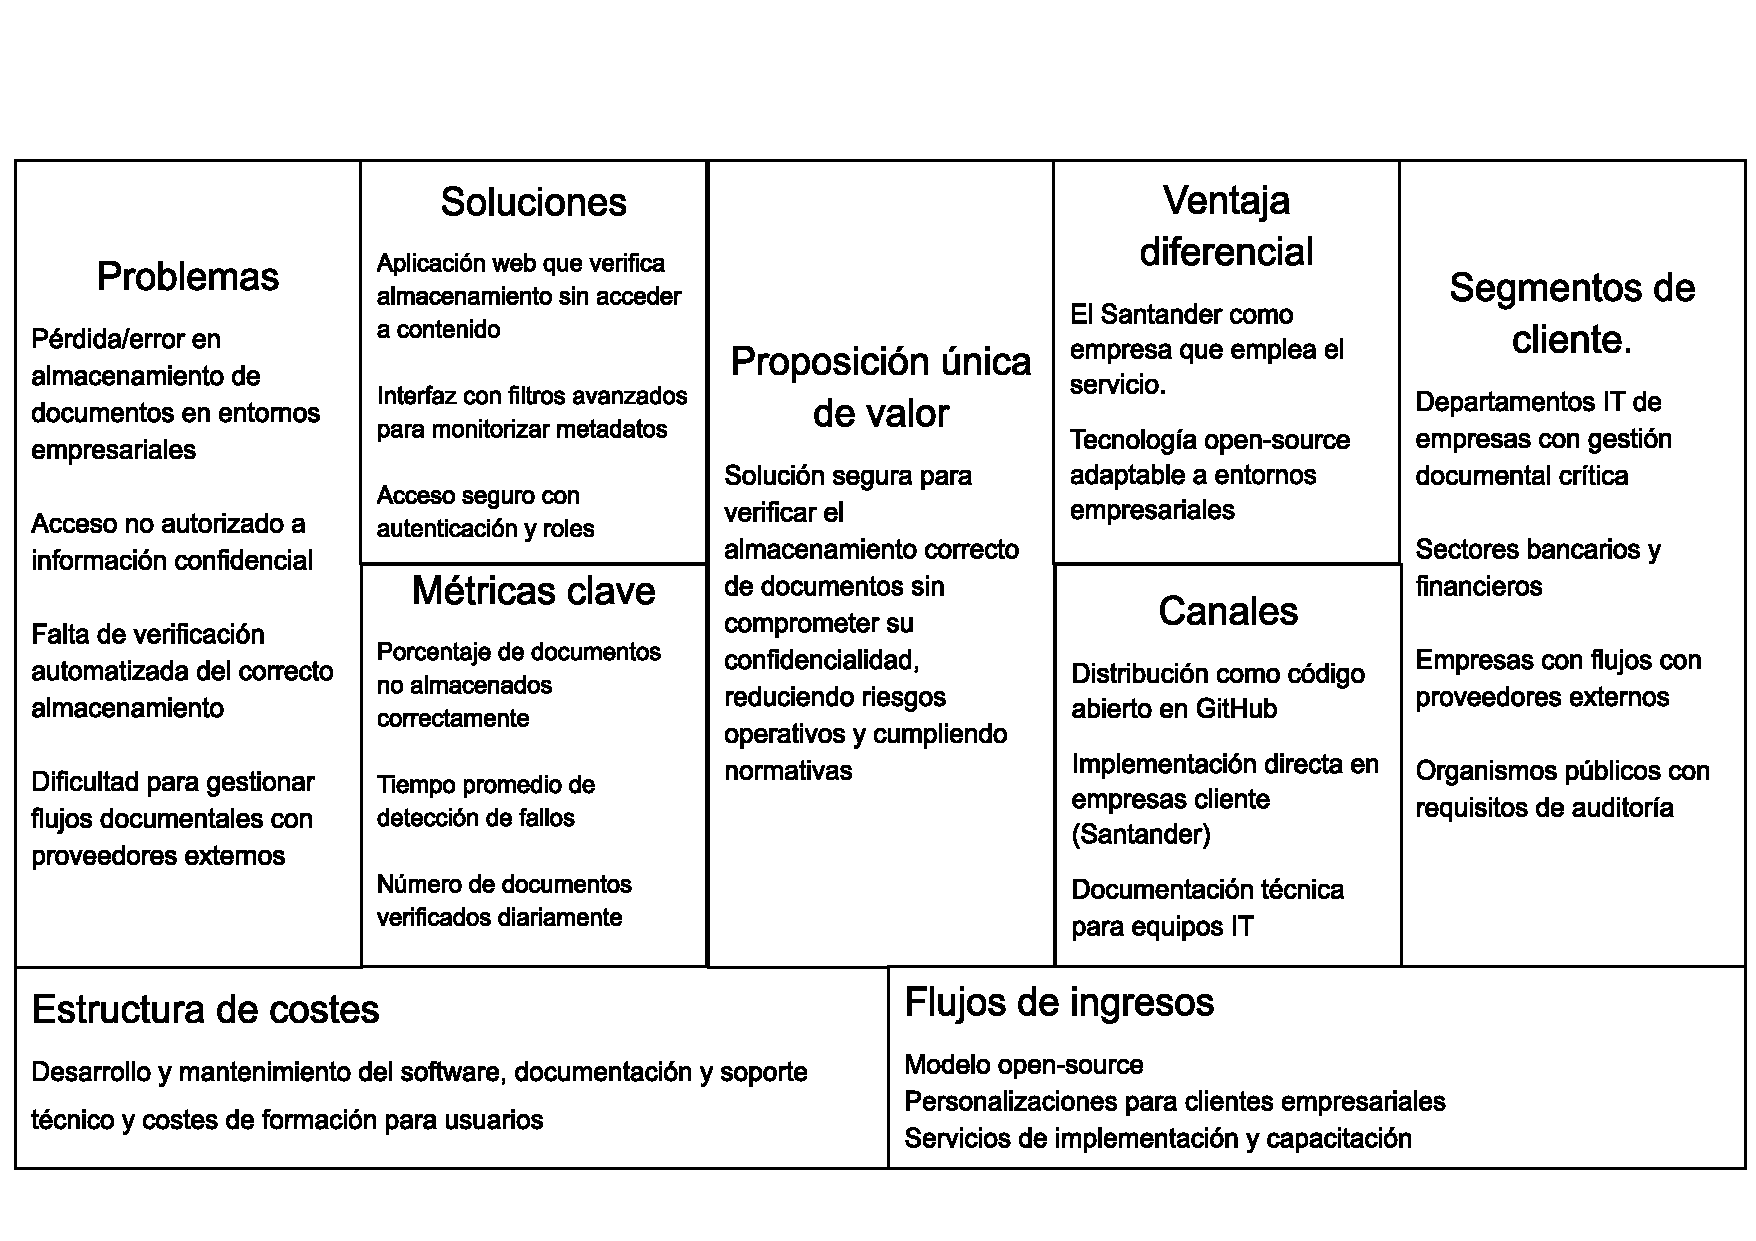
\includegraphics[width=1\linewidth]{imagenes/lean canvas tfg.pdf}
    \caption{Lean Canvas de SIDManager}
    \label{fig:lean-canvas}
\end{figure}

\subsection{Problemas identificados}
El canvas destaca cuatro problemáticas principales en la gestión documental empresarial:
\begin{itemize}
    \item Pérdidas y errores en el almacenamiento de documentos
    \item Riesgos de acceso no autorizado a información confidencial
    \item Falta de mecanismos automatizados para verificar el almacenamiento correcto
    \item Dificultades en la gestión de flujos documentales con proveedores externos
\end{itemize}

\subsection{Solución tecnológica}
La propuesta se articula en tres componentes fundamentales:
\begin{itemize}
    \item Aplicación web de verificación sin acceso a contenido confidencial
    \item Interfaz con sistema avanzado de filtrado de metadatos
    \item Arquitectura de seguridad con autenticación robusta y gestión de roles
\end{itemize}

\subsection{Métricas de éxito}
Se establecen tres indicadores clave de rendimiento (KPIs):
\begin{itemize}
    \item Tasa de documentos mal almacenados (\%)
    \item Tiempo medio de detección de anomalías
    \item Volumen diario de documentos verificados
\end{itemize}

\subsection{Propuesta de valor}
La singularidad de SIDManager radica en su capacidad para:
\begin{itemize}
    \item Garantizar la integridad documental sin comprometer la confidencialidad
    \item Reducir riesgos operativos en procesos críticos
    \item Cumplir con normativas de protección de datos (GDPR, etc.)
\end{itemize}

\subsection{Ventaja competitiva}
Dos factores diferenciadores:
\begin{itemize}
    \item Caso de uso real en entidad bancaria (Santander) como validación temprana
    \item Modelo open-source con adaptabilidad a entornos empresariales complejos
\end{itemize}

\subsection{Segmentación de clientes}
Los principales mercados objetivo incluyen:
\begin{itemize}
    \item Departamentos IT de empresas con gestión documental crítica
    \item Sector bancario y financiero (clientes primarios)
    \item Organismos públicos con exigentes requisitos de auditoría
    \item Empresas con flujos documentales externos complejos
\end{itemize}

\subsection{Modelo de distribución}
Estrategia multicanal:
\begin{itemize}
    \item Publicación como código abierto en GitHub
    \item Implementación directa en clientes corporativos
    \item Documentación técnica especializada para equipos IT
\end{itemize}

\subsection{Estructura económica}
\begin{itemize}
    \item Costes principales: Desarrollo de software, mantenimiento, soporte técnico y formación
    \item Flujos de ingresos: 
    \begin{itemize}
        \item Modelo open-source (versión base gratuita)
        \item Personalizaciones para clientes empresariales
        \item Servicios profesionales de implementación
    \end{itemize}
\end{itemize}

\section{Evaluación de riesgos}
Cada riesgo ha sido evaluado según dos parámetros fundamentales en la tabla \ref{table:risk-table}:
\begin{itemize}
    \item Probabilidad: Baja ( 0 - 30 \%), Moderada ( 30 - 70 \%), Alta ( 70 - 100 \%)
    \item Impacto: Tolerable (afecta plazos menores), Serio (compromete funcionalidades), Crítico (pone en peligro el proyecto)
\end{itemize}

\begin{table}
    \caption{Tabla de evaluación de riesgos}
    \label{table:risk-table}
    \begin{center}
    
    \begin{longtable}{|>{\raggedright\arraybackslash}p{3cm}|>{\raggedright\arraybackslash}p{3cm}|>{\raggedright\arraybackslash}p{2cm}|>{\raggedright\arraybackslash}p{6cm}|}
    \hline
    \textbf{Riesgo} & \textbf{Probabilidad} & \textbf{Efecto} & \textbf{Estrategia} \\
    \hline
    \endhead
    
    \hline
    \multicolumn{4}{|c|}{\textbf{Riesgos Tecnológicos}} \\
    \hline
    
    Desconocimiento al utilizar Spring Boot, JPA y Thymeleaf & Moderada & Tolerable & 
    \begin{itemize}
    \item Prevención: Realizar cursos y tutoriales sobre las tecnologías antes de comenzar el desarrollo
    \item Minimización: Consultar documentación oficial y ejemplos de proyectos similares
    \item Contingencia: Usar tecnologías alternativas más conocidas como Angular o React si fuera necesario
    \end{itemize} \\
    \hline
    
    Problemas de compatibilidad entre versiones de las tecnologías & Baja & Serio &
    \begin{itemize}
    \item Prevención: Verificar compatibilidad entre versiones antes de comenzar
    \item Minimización: Usar versiones LTS (Long Term Support) de las tecnologías
    \item Contingencia: Mantener versiones anteriores hasta resolver los conflictos
    \end{itemize} \\
    \hline
    
    Rendimiento insuficiente con grandes volúmenes de documentos & Moderada & Serio &
    \begin{itemize}
    \item Prevención: Diseñar consultas optimizadas y usar paginación
    \item Minimización: Implementar caché para consultas frecuentes
    \item Contingencia: Limitar el número de documentos mostrados por consulta
    \end{itemize} \\
    \hline
    
    \multicolumn{4}{|c|}{\textbf{Riesgos Personales}} \\
    \hline
    
    Falta de experiencia en desarrollo de aplicaciones empresariales & Alta & Tolerable &
    \begin{itemize}
    \item Prevención: Asignar tiempo extra para investigación y aprendizaje
    \item Minimización: Consultar con tutores y compañeros con más experiencia
    \item Contingencia: Simplificar funcionalidades complejas en primera iteración
    \end{itemize} \\
    \hline
    
    Problemas de gestión del tiempo & Moderada & Serio &
    \begin{itemize}
    \item Prevención: Crear un cronograma detallado con hitos claros
    \item Minimización: Usar metodologías ágiles con sprints cortos
    \item Contingencia: Priorizar funcionalidades esenciales para MVP
    \end{itemize} \\
    \hline
    
    \multicolumn{4}{|c|}{\textbf{Riesgos de Organización}} \\
    \hline
    
    Cambios en los requerimientos durante el desarrollo & Moderada & Serio &
    \begin{itemize}
    \item Prevención: Documentar exhaustivamente los requerimientos iniciales
    \item Minimización: Mantener comunicación constante con los stakeholders
    \item Contingencia: Usar diseño modular para facilitar cambios
    \end{itemize} \\
    \hline
    
    Dependencia de terceros (empresa colaboradora) & Baja & Crítico &
    \begin{itemize}
    \item Prevención: Establecer acuerdos claros desde el inicio
    \item Minimización: Mantener comunicación periódica
    \item Contingencia: Desarrollar versión simulada de los servicios externos
    \end{itemize} \\
    \hline
    
    \multicolumn{4}{|c|}{\textbf{Riesgos de Herramientas}} \\
    \hline
    
    Problemas con la configuración de Spring Security & Moderada & Serio &
    \begin{itemize}
    \item Prevención: Estudiar a fondo la documentación de Spring Security
    \item Minimización: Implementar configuración por pasos con pruebas intermedias
    \item Contingencia: Usar soluciones de autenticación más simples inicialmente
    \end{itemize} \\
    \hline
    
    Dificultades con la integración de Thymeleaf & Baja & Tolerable &
    \begin{itemize}
    \item Prevención: Realizar prototipos iniciales con Thymeleaf
    \item Minimización: Usar fragmentos reutilizables y layouts
    \item Contingencia: Considerar el uso de herramientas alternativas
    \end{itemize} \\
    \hline
    
    \multicolumn{4}{|c|}{\textbf{Riesgos de Requerimientos}} \\
    \hline
    
    Requerimientos de seguridad demasiado exigentes & Alta & Serio &
    \begin{itemize}
    \item Prevención: Analizar minuciosamente los requerimientos de seguridad
    \item Minimización: Implementar Spring Security desde el inicio del proyecto
    \item Contingencia: Priorizar las medidas de seguridad más críticas
    \end{itemize} \\
    \hline
    
    Dificultad en la validación de documentos sin acceder a metadatos & Moderada & Serio &
    \begin{itemize}
    \item Prevención: Estudiar alternativas técnicas para la validación
    \item Minimización: Consultar con expertos en seguridad de datos
    \item Contingencia: Proponer un método alternativo de verificación
    \end{itemize} \\
    \hline
    
    \multicolumn{4}{|c|}{\textbf{Otros Riesgos}} \\
    \hline
    
    Problemas con la base de datos en producción & Baja & Crítico &
    \begin{itemize}
    \item Prevención: Realizar copias de seguridad periódicas
    \item Minimización: Implementar scripts de migración y recuperación
    \item Contingencia: Tener un entorno de desarrollo independiente
    \end{itemize} \\
    \hline
    
    \end{longtable}
    \end{center}
\end{table}

\section{Conclusiones de viabilidad}
El análisis conjunto del Lean Canvas y la matriz de riesgos permite concluir que:
\begin{enumerate}
    \item El proyecto es técnicamente viable, aunque requiere inversión inicial en capacitación.
    \item La viabilidad económica está garantizada por el modelo de ingresos escalable.
    \item Los riesgos identificados son gestionables mediante las estrategias propuestas.
    \item El factor crítico de éxito reside en el equilibrio entre seguridad y usabilidad.
\end{enumerate}

Por tanto, el estudio demuestra que SIDManager aborda una necesidad real del mercado con una solución técnicamente robusta, posicionándose como una alternativa viable frente a soluciones existentes como Alfresco o OpenKM. Los siguientes capítulos detallarán la implementación concreta de las estrategias aquí esbozadas.

\chapter{Estado de la cuestión}
El desarrollo de sistemas de gestión y monitorización de documentos es un área de gran relevancia en el ámbito empresarial, especialmente en sectores donde la integridad y disponibilidad de la información son críticas. En este capítulo, se analiza el impacto de la pérdida de documentos, las iniciativas existentes para su monitorización y las tecnologías web más utilizadas en la actualidad.

Aquí tienes la sección ampliada con los cambios solicitados, incorporando mayor detalle y referencias bibliográficas:


\section{Impacto y costes de la pérdida de documentos}
La gestión documental efectiva constituye un pilar fundamental en la operativa empresarial moderna, donde la digitalización y el volumen de información generada plantean desafíos crecientes. Una gestión inadecuada puede desencadenar consecuencias devastadoras tanto a nivel operativo como legal y reputacional.

\subsection{Riesgos en el ciclo de vida documental}
El proceso de gestión de documentos implica múltiples etapas críticas donde pueden producirse fallos. Según \citetitle{ISO15801:2017}, hasta el 43\% de las pérdidas documentales ocurren durante las fases de transferencia o almacenamiento temporal. Un riesgo particular surge cuando la generación de documentos se delega a proveedores externos, práctica común en sectores como el legal. Este outsourcing introduce vulnerabilidades al:

\begin{itemize}
    \item Multiplicar los puntos de contacto en el flujo documental
    \item Requerir protocolos de transferencia seguros entre sistemas heterogéneos
    \item Dificultar la auditoría de trazabilidad completa
\end{itemize}

\subsection{Consecuencias operativas y regulatorias}
En el ámbito empresarial, la falta de acceso a información crítica genera interrupciones en cadena. Los costes asociados, como detalla el informe \citetitle{IBM2024}, incluyen:

\begin{itemize}
    \item Costes directos de recuperación (€35.000-€250.000 por incidente)
    \item Multas regulatorias (hasta 4\% del volumen de negocio anual bajo GDPR)
    \item Litigios por incumplimiento contractual
\end{itemize}

Sectores regulados como el bancario o sanitario enfrentan riesgos amplificados. La pérdida de documentos que contengan datos personales compromete no solo la privacidad, sino que genera responsabilidades legales escalonadas. El análisis de \textcite{cost-doc-manag-2020} revela que el 23\% de las brechas en estos sectores se originan en fallos de gestión documental, con costes medios por registro comprometido entre €350-€700.


\section{Otras iniciativas}
Ante la necesidad de garantizar la disponibilidad y seguridad de los documentos, se han desarrollado diversas iniciativas para su monitorización y gestión. Entre las más comunes se encuentran:

\begin{itemize}
    \item \textbf{Soluciones Open Source }: Dos de las aplicaciones Open Source más conocidas para la gestión de documentos son Alfresco y OpenKM.
    Alfresco es un sistema de gestión documental open source desarrollado en Java. Su versión Community es gratuita pero requiere especialistas para su implementación. Aunque ofrece potentes APIs de integración, su versión Enterprise tiene costos prohibitivos para medianas empresas \parencite{Evoltia2023}. 
    Por otro lado cabe destacar que las soluciones open source preexistentes requieren conocimientos técnicos avanzados para su implementación y mantenimiento.
    
    Por otro lado, OpenKM es una plataforma libre con interfaz web basada en tecnologías Java. Su versión Community sigue el modelo GPLv2, pero las versiones Professional y Cloud son comerciales. Aunque ofrece búsqueda avanzada y flujos de trabajo, su escalabilidad en entornos complejos es limitada \parencite{OpenKM2023}.
    
    \item Plataformas cloud comerciales (OneDrive/Google Drive):
    Soluciones SaaS fáciles de implementar pero con limitaciones en control de datos, cumplimiento normativo para sectores regulados y dependencia del proveedor. Carecen de funcionalidades avanzadas de gestión documental como workflows complejos o metadata estructurada. La principal desventaja de las plataformas cloud comerciales es que carecen de control sobre los datos y no cumplen con regulaciones estrictas.

    \item Sistemas de monitorización mediante scripts: Soluciones basadas en scripts personalizados que verifican el estado de los documentos en una base de datos. Aunque son flexibles y de bajo coste, su mantenimiento puede ser complejo y no suelen escalar bien en entornos con grandes volúmenes de datos.
    
    \item Bases de datos duplicadas: Estrategia que consiste en mantener copias redundantes de los documentos en diferentes servidores. Aunque mejora la disponibilidad, implica un mayor coste de almacenamiento y puede complicar la sincronización entre las bases de datos.
    
    \item Consultas \acrshort{sql} básicas: Uso de consultas \acrfull{sql} para verificar el estado de los documentos. Esta aproximación es sencilla pero limitada, ya que no ofrece funcionalidades avanzadas como la generación de informes o la integración con otras herramientas.
\end{itemize}

Estas iniciativas, aunque útiles en ciertos contextos, presentan limitaciones en términos de escalabilidad, seguridad y facilidad de uso, lo que justifica la necesidad de soluciones más avanzadas como SIDManager.

%--------------------------
\section{Tecnologías web}
%--------------------------
El desarrollo de aplicaciones web modernas requiere la selección de tecnologías adecuadas que permitan construir sistemas eficientes, seguros y escalables.

En este contexto, conviene distinguir entre un script y una aplicación web. Un \emph{script} es un conjunto de instrucciones escritas en un lenguaje de programación (como Python o bash) que se ejecutan de manera secuencial para realizar tareas específicas. Aunque son útiles para automatizar procesos, los scripts suelen carecer de una interfaz de usuario y no están diseñados para manejar grandes volúmenes de datos o usuarios concurrentes.

En cambio, una \emph{aplicación web} \parencite{AWS2025} es un sistema completo que incluye una interfaz de usuario, lógica de negocio y persistencia de datos. Las aplicaciones web están diseñadas para ser accesibles desde navegadores y suelen utilizar tecnologías como \acrfull{html}, \acrfull{css}, JavaScript en el front-end, y frameworks como Spring Boot o Django en el backend. A diferencia de los scripts, las aplicaciones web son escalables, seguras y ofrecen una experiencia de usuario más completa.
En este capítulo  se analizan las tecnologías más relevantes en este último ámbito.
 

\subsection{Metodos HTTP }

Como sostiene la \textcite{MDN_HTTP_Methods}, los métodos HTTP (HyperText Transfer Protocol) son la base de la comunicación en la web y definen las operaciones que se pueden realizar sobre los recursos. Los más utilizados son los métodos \acrshort{get} y los métodos \acrshort{post}.

Un método GET se utiliza para solicitar datos de un recurso específico. Es idempotente, lo que significa que múltiples solicitudes GET no modifican el estado del servidor. Este método es ideal para recuperar información, como listados de documentos o detalles de un usuario.

Por contra, un
método POST se utiliza para enviar datos al servidor, generalmente para crear nuevos recursos. A diferencia de GET, POST no es idempotente, ya que cada solicitud puede generar un cambio en el servidor. Este método es común en formularios de registro o envío de datos.

\subsection{API}
Una \acrfull{api} es un conjunto de reglas y protocolos que permite la comunicación entre diferentes sistemas. Las APIs son fundamentales en el desarrollo de aplicaciones modernas, ya que facilitan la integración entre servicios y permiten construir sistemas modulares y escalables.

\subsection{REST}
\acrfull{rest} es un estilo arquitectónico para diseñar APIs web. Se basa en el uso de métodos HTTP (GET, POST, \acrshort{put}, DELETE) para realizar operaciones sobre recursos identificados por \acrshort{url}s. REST es ampliamente utilizado debido a su simplicidad, escalabilidad y compatibilidad con diferentes tecnologías. Además, las APIs RESTful son fáciles de consumir desde clientes web, móviles o de escritorio, lo que las convierte en una opción ideal para aplicaciones como SIDManager.


\section{Herramientas para el desarrollo }

En este capítulo se describen las principales tecnologías y herramientas utilizadas en el desarrollo de esta aplicación web, analizando su origen, propósito y cómo contribuyen al proyecto.

\subsection{Angular}

Tal y como explica \textcite{Zurawski2024}, Angular 
es un framework de desarrollo web creado por Google en 2010, diseñado para facilitar la construcción de aplicaciones de una sola página (\acrshort{spa}) en el lado del cliente. Estaba basado en JavaScript, así se ve en \citetitle{javascript} de \citeauthor{javascript}
 pero desde la versión 2, tanto internamente en la aplicación como para hacer desarrollos con esta, se utiliza TypeScript \parencite{typescript}
 un superconjunto de JavaScript que añade tipado estático, mejorando la robustez y escalabilidad de las aplicaciones desarrolladas con Angular.
El principal propósito de Angular es simplificar la creación de interfaces de usuario dinámicas y reactivas, permitiendo que los desarrolladores gestionen el contenido de forma más eficiente. Su arquitectura basada en componentes y el uso de un sistema de inyección de dependencias hacen que Angular sea muy adecuado para grandes aplicaciones front-end. Además, ofrece un sistema de dos vías de enlace de datos (two-way data binding) que sincroniza de manera automática los cambios entre el modelo y la vista.

\begin{figure}
    \centering
    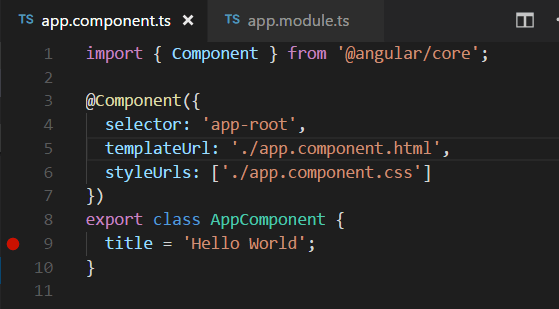
\includegraphics[width=0.75\linewidth]{imagenes/code/angular_components.png}
    \caption{Ejemplo de componentes de Angular con código Typescript. }
    \label{fig:angular_components}
\end{figure}

Angular es parte de un conjunto más amplio de herramientas y tecnologías de Google, por lo que su integración con otros servicios de Google es fluida. A lo largo de los años, ha ganado popularidad en el desarrollo front-end, especialmente en entornos empresariales, debido a su capacidad para manejar aplicaciones de gran escala y su enfoque en la modularidad y reutilización de código.

Uno de los lenguajes que se utiliza en Angular es TypeScript, que proporciona características de programación orientada a objetos como clases, interfaces y herencia, facilitando el desarrollo de aplicaciones más mantenibles. Este lenguaje lo hace ideal para proyectos de gran tamaño, donde el control de tipos puede ayudar a reducir errores. A pesar de ser un framework basado en el front-end, Angular puede integrarse con varios backends, como Node.js, Django, Spring, entre otros.

Angular es un framework respaldado por Google, lo que asegura un ciclo de vida estable y una comunidad activa que contribuye a su mejora continua. Además, dado que Angular es open-source, la comunidad también juega un papel clave en su evolución, lo que garantiza que el framework continúe siendo relevante en la industria del desarrollo web.

Aunque Angular es muy popular, su curva de aprendizaje puede ser algo pronunciada, especialmente para desarrolladores novatos. Además, debido a su carácter completo, puede ser excesivo para aplicaciones más pequeñas, donde un framework más ligero podría ser suficiente. Sin embargo, en proyectos de gran escala que requieren una estructura bien organizada y mantenible, Angular sigue siendo una opción sólida.

\subsection{React}
React es una biblioteca de JavaScript para la construcción de interfaces de usuario, desarrollada por Facebook (ahora Meta), como se puede apreciar en el artículo \citetitle{facebook},
y lanzada al público en 2013. Su principal propósito es facilitar el desarrollo de aplicaciones web interactivas y reactivas mediante un enfoque basado en componentes reutilizables. 

React se enfoca en la parte de la vista (view) en el patrón de diseño 
\acrfull{mvc} como explica \citeauthor{MVC} en el estudio \citetitle{MVC}, lo que permite crear interfaces dinámicas sin tener que recargar la página web.

Una de las características más destacadas de React es su uso del \acrfull{vdom} tal y como explica en \citetitle{virtual-dom}. Este artículo sostiene que se obtiene una mejora significativa en el rendimiento al minimizar la manipulación directa del DOM del navegador. En lugar de modificar el DOM completo con cada cambio, React crea una copia de este en memoria y solo actualiza las partes que han cambiado, lo que hace que las aplicaciones sean más rápidas y eficientes.

\begin{figure}
    \centering
    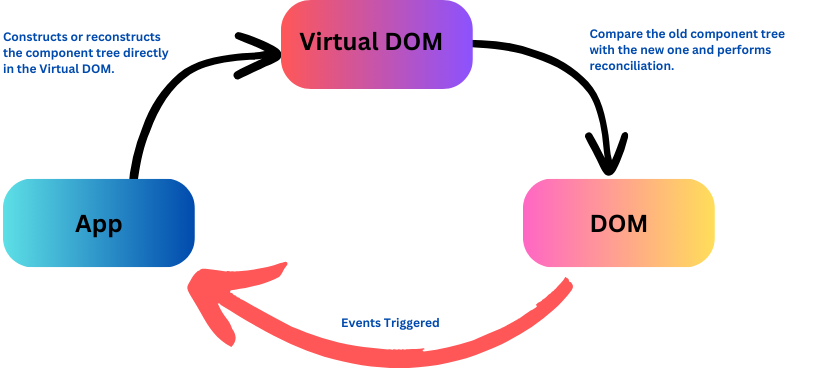
\includegraphics[width=0.75\linewidth]{imagenes/scheme/react_virtual_dom.png}
    \caption{Ejemplo de DOM virtual de React hecho por \textcite{virtual-dom-scheme}}
    \label{fig:react_virtual_dom}
\end{figure}

React está escrito en JavaScript, pero con soporte extendido para \acrfull{jsx} (para más información, ver el informe de \citeauthor{JSX} llamado \citetitle{JSX})
una extensión de sintaxis que permite escribir elementos de la interfaz de usuario de forma declarativa, como si fueran parte del código HTML. Esto facilita a los desarrolladores visualizar claramente la estructura del componente dentro del código JavaScript, simplificando el desarrollo y mantenimiento de la interfaz.

El ecosistema de React ha crecido enormemente desde su lanzamiento. Aunque originalmente fue concebido para aplicaciones de una sola página (SPA), React ha evolucionado para ser usado tanto en el desarrollo front-end como en aplicaciones móviles, mediante el uso de React Native. Esto convierte a React en una tecnología versátil, usada en una amplia variedad de plataformas.

Una ventaja importante de React es su flexibilidad: no impone una arquitectura rígida y se puede integrar fácilmente con otras bibliotecas o frameworks. 

A pesar de sus ventajas, React tiene algunas desventajas. Una de ellas es que, aunque es fácil de aprender para pequeños proyectos, gestionar el estado en aplicaciones grandes puede volverse complicado, lo que requiere el uso de bibliotecas externas como Redux o Context API. Además, React es solo una biblioteca para la vista, lo que significa que carece de muchas funcionalidades de un framework completo, como el enrutamiento o la gestión de dependencias, que deben añadirse manualmente.

React ha ganado una enorme popularidad desde su lanzamiento y sigue siendo una de las bibliotecas más utilizadas para el desarrollo web, debido a su eficiencia, flexibilidad y soporte por parte de una comunidad muy activa.

\subsection{ Spring }
Spring es un marco de trabajo (framework) para el desarrollo de aplicaciones en Java, como sostiene \cite{spring-def}
, ampliamente utilizado en entornos empresariales debido a su flexibilidad y capacidad para facilitar el desarrollo de aplicaciones robustas y escalables. Fue desarrollado por Rod Johnson y lanzado inicialmente en 2003, como una alternativa ligera a los frameworks Java más pesados de la época. Spring permite construir aplicaciones que siguen los principios de inyección de dependencias y programación orientada a aspectos (para más detalle sobre programación orientada a objetos ver \textcite{aop})
, lo que mejora la modularidad y facilita la gestión de la complejidad en proyectos grandes.



El propósito principal de Spring es simplificar el desarrollo de aplicaciones en Java, proporcionando una infraestructura sólida que resuelve los problemas comunes en la creación de aplicaciones de servidor. Además de su flexibilidad, Spring se destaca por sus capacidades de integración con otros frameworks y tecnologías, lo que lo convierte en una solución versátil para la creación de aplicaciones web, \gls{api}
y microservicios.

Spring es el framework base que se extiende a través de módulos como Spring MVC (para aplicaciones web), Spring Security (para control de acceso) y Spring Data (para gestión de bases de datos). Gracias a su popularidad, sigue siendo el framework Java más utilizado para el desarrollo de aplicaciones empresariales.

\subsection{ Spring Boot }
Spring Boot es una extensión del framework Spring que fue publicada en 2014 por Pivotal Software. Está diseñada para simplificar el proceso de configuración y arranque de las aplicaciones desarrolladas en Spring. Mientras que Spring ofrece una gran flexibilidad, su configuración puede ser tediosa y propensa a errores. Aquí es donde Spring Boot aporta su valor: reduce la necesidad de configuración manual gracias a las convenciones predeterminadas y a una serie de herramientas integradas como \acrfull{jpa} (que explicaremos más adelante), Spring Web \parencite{spring-security} y muchas más.

Spring Boot permite a los desarrolladores centrarse en la lógica del negocio en lugar de en la configuración del entorno, ya que automatiza la mayor parte de la configuración, incluyendo el servidor web, la integración con bases de datos y la seguridad. Esto es posible gracias a la división en las capas: vista (view) o cliente (client), controlador (controller), servicio (service), modelo (model) y repositorio (repository) entre otras, como se ve en la figura ~\ref{fig:spring_boot_layers}. 
Esto lo convierte en una excelente opción para la creación rápida de prototipos, aplicaciones de producción listas para el despliegue y microservicios. Su popularidad ha crecido rápidamente debido a la eficiencia que proporciona, lo que ha hecho que muchos desarrolladores lo elijan para proyectos grandes y pequeños.


\begin{figure}
        \centering
        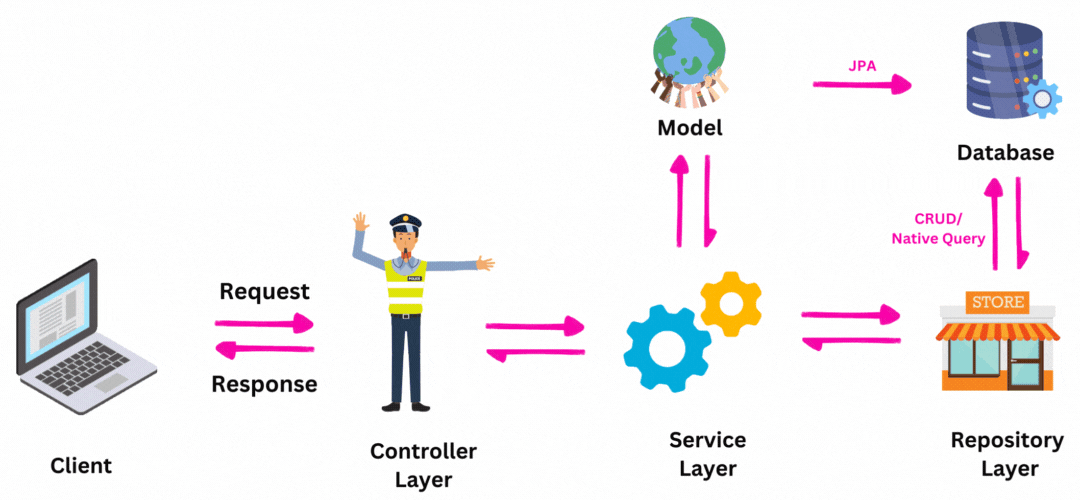
\includegraphics[width=0.75\linewidth]{imagenes/scheme/spring_boot_layers.png}
        \caption{Capas de Spring Boot hecho por \textcite{spring-layers}}
        \label{fig:spring_boot_layers}
    \end{figure}



Spring Boot se integra fácilmente con otros componentes de Spring, como Spring Security y Spring Data, y se basa en las mismas buenas prácticas que han hecho de Spring un estándar en la industria del desarrollo de software. Por ejemplo, Spring Boot facilita la integración con JPA, el cual permite la persistencia de datos en bases de datos relacionales.

\subsection{ JPA }

JPA (Java Persistence API) es una especificación que simplifica la interacción con bases de datos en aplicaciones Java. Fue introducida en 2006 como parte de la plataforma \acrfull{javaee} 5 y desarrollada por Oracle. Su objetivo es facilitar el mapeo de objetos Java a tablas de bases de datos relacionales sin la necesidad de escribir SQL manualmente. Con JPA, los desarrolladores pueden centrarse en el código de negocio sin preocuparse por los detalles de la persistencia, como se ve en el artículo de \textcite{jpa-spring-integration}.

Una de las grandes ventajas de JPA es que reduce la cantidad de código repetitivo necesario para realizar operaciones \acrfull{crud} en la base de datos. 

JPA permite que los desarrolladores trabajen con objetos de dominio directamente, delegando la gestión de las transacciones y el acceso a la base de datos en el framework subyacente. En combinación con Spring Data JPA, la interacción con la base de datos se hace más sencilla y eficiente, eliminando la necesidad de escribir consultas SQL explícitas en la mayoría de los casos.

JPA se utiliza principalmente en aplicaciones que requieren una gestión compleja de datos, y su integración con Spring Boot a través de Spring Data JPA permite acelerar el desarrollo al proporcionar un enfoque estandarizado para la persistencia de datos.



\subsection{ Maven }

Maven es una herramienta de gestión de proyectos y de automatización de construcción para aplicaciones Java, desarrollada por la Apache Software Foundation y lanzada en 2004 \parencite{maven-official}.

Su principal función es gestionar las dependencias de un proyecto, es decir, todas las bibliotecas externas que el proyecto necesita para funcionar. Maven permite a los desarrolladores definir estas dependencias en un archivo \acrfull{xml} llamado pom.xml y luego descarga automáticamente las versiones correctas de estas bibliotecas desde repositorios remotos.

Una de las mayores ventajas de Maven es su capacidad para estandarizar el proceso de construcción de aplicaciones Java, independientemente del entorno en el que se desarrolle. Esto asegura que los proyectos construidos con Maven sean consistentes y que se puedan replicar fácilmente en cualquier máquina de desarrollo.

En este proyecto, Maven juega un papel crucial al manejar las dependencias de Spring Boot, JPA y Thymeleaf, asegurando que todas las bibliotecas necesarias estén disponibles y configuradas correctamente.

\subsection{ Thymeleaf }
\label{subsec:thymeleaf}

Thymeleaf es un motor de plantillas para aplicaciones Java, creado por Daniel Fernández en 2011, que permite la generación dinámica de contenido HTML, XML y otros formatos de texto, tal y como lo explican sus creadores en la web oficial \textcite{thymeleaf-official}.

Thymeleaf se usa principalmente para construir la vista (view) o plantilla (template) en aplicaciones web, y es altamente compatible con Spring, ya que facilita la integración de los modelos de datos Java con las plantillas HTML de manera eficiente.

Una de las principales ventajas de Thymeleaf es que permite crear plantillas que pueden ser previsualizadas sin necesidad de ejecutar la aplicación en un servidor. Esto lo hace particularmente útil para el desarrollo colaborativo entre diseñadores y programadores, ya que los archivos HTML son completamente editables desde el lado del cliente.

Thymeleaf está diseñado para funcionar bien con Spring MVC y Spring Boot, lo que lo convierte en una opción natural para las aplicaciones web que necesitan generar contenido dinámico basado en datos proporcionados por el servidor.


    



    
\section{Ciberseguridad}
\label{sec:ciberseguridad}

La ciberseguridad es un aspecto crítico en el desarrollo de aplicaciones modernas, especialmente cuando se manejan datos sensibles como credenciales de usuarios, información personal, contraseñas y documentos privados. En este apartado, se describen las tecnologías y prácticas más relevantes en el ámbito de la ciberseguridad, con un enfoque en el cifrado de datos y las capas de seguridad en el proceso de autenticación.

El cifrado es una técnica fundamental para proteger la confidencialidad e integridad de los datos. Consiste en transformar la información en un formato ilegible para cualquier persona que no posea la clave de descifrado adecuada. A continuación, se describen los principales enfoques y tecnologías utilizadas en el cifrado de datos.

\subsection{Cifrado simétrico}

El cifrado simétrico \parencite{symmetric-encryption} utiliza una única clave para cifrar y descifrar los datos. Este enfoque es eficiente en términos de rendimiento, ya que requiere menos recursos computacionales en comparación con el cifrado asimétrico. Sin embargo, la gestión segura de la clave es un desafío, ya que debe compartirse entre las partes que necesitan cifrar y descifrar los datos.

 AES (\emph{Advanced Encryption Standard}) es uno de los algoritmos de cifrado simétrico más utilizados y seguros. AES opera en bloques de 128 bits y admite claves de 128, 192 o 256 bits. Su fortaleza radica en su resistencia a ataques criptográficos y su eficiencia en términos de velocidad.
 
  AES puede utilizarse en diferentes modos de operación, como \acrfull{ecb}, \acrfull{cbc} y \acrfull{gcm}. Cada modo tiene sus propias características y niveles de seguridad.


\subsection{Cifrado asimétrico}

El cifrado asimétrico, también conocido como cifrado de clave pública, utiliza un par de claves: una clave pública para cifrar los datos y una clave privada para descifrarlos. Este enfoque es ideal para escenarios donde la clave no puede compartirse de manera segura, como en la comunicación entre dos partes que no han establecido previamente una relación de confianza.

 \acrfull{rsa} es uno de los algoritmos de cifrado asimétrico más populares. RSA se basa en la dificultad de factorizar números grandes en sus componentes primos. Aunque es seguro, su rendimiento es inferior al cifrado simétrico, por lo que se utiliza principalmente para cifrar claves o datos pequeños.
   
 \emph{Curvas Elípticas} \acrfull{ecc} es una alternativa más moderna y eficiente a RSA. ECC ofrece un nivel de seguridad similar con claves más cortas, lo que reduce el consumo de recursos y mejora el rendimiento.


\subsection{Cifrado de contraseñas}

El cifrado de contraseñas es un caso especial donde se utilizan funciones de hash unidireccionales para almacenar las contraseñas de manera segura. A diferencia del cifrado tradicional, el hash no puede revertirse, lo que garantiza que incluso si la base de datos es comprometida, las contraseñas no puedan recuperarse.

\begin{itemize}
    \item BCrypt: Es una función de hash diseñada específicamente para contraseñas. BCrypt utiliza un valor de \emph{salt} \parencite{salt} único para cada contraseña, lo que aumenta la seguridad frente a ataques de diccionario y fuerza bruta. Además, su diseño permite ajustar la complejidad del hashing, lo que lo hace resistente a los avances en hardware.
    \item Argon2: Es una función de hash moderna que ha ganado popularidad debido a su resistencia a ataques de fuerza bruta y su capacidad para utilizar múltiples recursos del sistema (\acrshort{cpu}, memoria y paralelismo). Argon2 es considerado uno de los algoritmos más seguros para el cifrado de contraseñas.
\end{itemize}

\subsection{Capas de Seguridad en el login}
\label{subsec:capas-seguridad-login}

El proceso de autenticación es uno de los puntos más vulnerables en cualquier aplicación, ya que es el primer paso para acceder a los recursos protegidos. Para garantizar la seguridad del login, es esencial implementar múltiples capas de seguridad que protejan contra ataques comunes y refuercen la integridad del sistema.


Los ataques de fuerza bruta intentan adivinar las credenciales de un usuario probando múltiples combinaciones de nombres de usuario y contraseñas. Para proteger contra estos ataques, es esencial implementar medidas como:

\begin{itemize}
    \item Límite de Intentos: Bloquear temporalmente la cuenta después de un número determinado de intentos fallidos. Esto dificulta que un atacante pueda probar múltiples combinaciones en un corto período de tiempo.
    \item CAPTCHA: Requerir que el usuario resuelva un desafío \acrshort{captcha} después de varios intentos fallidos. Esto ayuda a distinguir entre usuarios legítimos y bots automatizados.
\end{itemize}

Los ataques \acrfull{csrf} explotan la confianza que un sitio web tiene en el navegador del usuario para realizar acciones no autorizadas. Para prevenir estos ataques, se pueden implementar las siguientes medidas:

\begin{itemize}
    \item Tokens CSRF: Generar un token único para cada sesión de usuario y validarlo en cada solicitud. Esto garantiza que la solicitud proviene de una fuente legítima.
    \item SameSite Cookies: Configurar las cookies con el atributo SameSite para evitar que se envíen en solicitudes cruzadas entre sitios.
\end{itemize}


El registro y monitoreo de la actividad del usuario es esencial para detectar y responder a posibles amenazas de seguridad. Algunas prácticas recomendadas incluyen:

\begin{itemize}
    \item Registro de Accesos: Registrar todos los intentos de login, tanto exitosos como fallidos, para identificar patrones sospechosos.
    \item Alertas de Seguridad: Configurar alertas para notificar a los administradores en caso de actividades inusuales, como múltiples intentos fallidos de login desde diferentes ubicaciones.
\end{itemize}


\section{Diseño software}
El diseño de software es una fase crítica en el desarrollo de aplicaciones, ya que define la estructura, organización y comportamiento del sistema. Un buen diseño no solo garantiza que el software cumpla con los requisitos funcionales, sino que también facilita su mantenimiento, escalabilidad y reutilización. En este apartado, se abordarán los patrones de diseño más comunes y los diagramas \acrfull{uml}, herramientas esenciales para modelar y documentar sistemas de software.

\subsection{Patrones de diseño software}
Los patrones de diseño son soluciones probadas y reutilizables para problemas comunes en el desarrollo de software. Estos patrones proporcionan un enfoque estructurado para resolver desafíos específicos, mejorando la calidad del código y facilitando su mantenimiento. Para más información se puede obtener el libro de \textcite{design-patterns}. A continuación, se describen algunos de los patrones más utilizados:


El patrón Fachada es un patrón estructural que proporciona una interfaz simplificada para un conjunto de interfaces en un subsistema. Este patrón es útil cuando un sistema es complejo y tiene múltiples componentes, ya que oculta la complejidad detrás de una interfaz única y fácil de usar. Por ejemplo, en una aplicación con múltiples servicios y bibliotecas, una fachada puede actuar como un punto de entrada único, reduciendo la dependencia entre los componentes y facilitando su uso.


El patrón Singleton es un patrón creacional que garantiza que una clase tenga una única instancia y proporciona un punto de acceso global a esa instancia. Este patrón es útil cuando se necesita un único punto de control, como en la gestión de configuraciones, conexiones a bases de datos o registros de logs. Al garantizar que solo exista una instancia, se evita la duplicación de recursos y se asegura un comportamiento consistente en toda la aplicación.


Además de los mencionados, existen otros patrones ampliamente utilizados, como:
\begin{itemize}
    \item Patrón Observador (Observer): Permite que un objeto notifique a otros objetos sobre cambios en su estado.
    \item Patrón Estrategia (Strategy): Define una familia de algoritmos, encapsula cada uno de ellos y los hace intercambiables.
    \item Patrón Inyección de Dependencias (Dependency Injection): Facilita la gestión de dependencias entre componentes, promoviendo un código más modular y testeable.
\end{itemize}

\subsection{Diagramas UML}
El Lenguaje Unificado de Modelado (UML, por sus siglas en inglés) es un estándar utilizado para visualizar, especificar, construir y documentar sistemas de software. Los diagramas UML son una herramienta esencial para comunicar el diseño del software entre desarrolladores, analistas y stakeholders. A continuación, se describen los tipos de diagramas más relevantes.

Muchos artículos hablan del diagrama de secuencia UML como \textcite{uml-secuence-article}. Estos explican que el diagrama de secuencia es un tipo de diagrama de interacción que muestra cómo los objetos interactúan en un escenario específico a lo largo del tiempo. Este diagrama es especialmente útil para modelar el flujo de mensajes entre objetos en un sistema, lo que permite entender cómo se ejecutan las operaciones y en qué orden.

\begin{itemize}
    \item Actores: Representan los roles externos que interactúan con el sistema, como usuarios o sistemas externos.
    \item Objetos: Representan las instancias de clases o componentes del sistema.
    \item Mensajes: Representan las interacciones entre objetos, mostrando el flujo de control y datos.
    \item Línea de vida: Muestra la existencia de un objeto durante el tiempo de ejecución.
\end{itemize}

Los diagramas de secuencia son ideales para modelar casos de uso complejos, como procesos de autenticación, transacciones o flujos de trabajo. Además, son una herramienta valiosa para identificar cuellos de botella y optimizar el rendimiento del sistema.

Además del diagrama de secuencia, UML incluye otros tipos de diagramas, como:
\begin{itemize}
    \item Diagrama de clases: Muestra la estructura estática del sistema, incluyendo clases, atributos, métodos y relaciones.
    \item Diagrama de casos de uso: Representa las interacciones entre los actores y el sistema, describiendo las funcionalidades desde la perspectiva del usuario.
    \item Diagrama de actividades: Modela el flujo de trabajo o procesos de negocio, mostrando las actividades y decisiones involucradas.
    \item Diagrama de componentes: Muestra la organización física del sistema, incluyendo módulos, bibliotecas y dependencias.
\end{itemize}

En resumen, los patrones de diseño y los diagramas UML son herramientas fundamentales en el desarrollo de software moderno. Los patrones de diseño proporcionan soluciones reutilizables para problemas comunes, mientras que los diagramas UML facilitan la comunicación y documentación del diseño del sistema. Juntos, permiten crear aplicaciones robustas, mantenibles y escalables.

%
%Objetivos
\chapter{Objetivos} \label{objetivos}
El objetivo general de este proyecto es el diseño y desarrollo de una aplicación web para la gestión eficiente de documentos en una organización, facilitando conocer su estado y si han sido almacenados o no. Además, mediante el uso de filtros avanzados, los usuarios podrán identificar y gestionar de manera eficiente los metadatos de estos documentos, mejorando así la integridad y el control de la información. 
La aplicación también será escalable y segura, garantizando su adecuado funcionamiento en diversos entornos y proporcionando una herramienta útil para la gestión de bases de datos.

Los objetivos específicos del proyecto son:
\begin{enumerate}
    \item Desarrollar una interfaz web altamente usable. El diseño de la interfaz será intuitivo y accesible, permitiendo que cualquier usuario, independientemente de su nivel de conocimientos técnicos, pueda interactuar con la aplicación sin dificultad. Esto facilitará su adopción en empresas de distintos tamaños y sectores.

    \item Implementar un sistema basado en arquitectura cliente-servidor para ordenador. La aplicación será accesible a través de un navegador web, sin necesidad de instalación en dispositivos locales. Funcionará bajo una arquitectura cliente-servidor, donde el servidor aloja y gestiona los datos, mientras que los usuarios interactúan con la aplicación desde el cliente, facilitando así su uso en múltiples dispositivos y plataformas, sin las limitaciones de una aplicación de escritorio.
    
    \item Implementar mecanismos de seguridad avanzados. La aplicación incorporará diversas capas de seguridad, incluyendo autenticación de usuarios y cifrado robusto para proteger las credenciales. Se prestará especial atención a la prevención de vulnerabilidades, mediante el uso de sesiones seguras, códigos aleatorios y la gestión adecuada de estados.
    
    \item Optimizar la eficiencia y rendimiento de la aplicación. Se aplicarán técnicas y buenas prácticas para minimizar los tiempos de carga y garantizar que la aplicación funcione de manera rápida y eficiente, incluso cuando se maneje un gran volumen de datos.

    \item Generar un código limpio, modular y bien documentado. El código será diseñado para ser fácilmente reusable y mantenible, con una arquitectura desacoplada que permita modificar los inputs desde archivos externos. Además, se integrarán logs exhaustivos y documentación clara para facilitar futuras mejoras y el trabajo de otros desarrolladores.

    \item Aplicar diagramas de secuencia UML. Para garantizar un desarrollo estructurado y coherente, se emplearán diagramas de secuencia UML, permitiendo una planificación detallada de los flujos de trabajo y las interacciones entre los componentes del sistema.

\end{enumerate}

%\chapter{Metodología y entorno de desarrollo}

Este capítulo detalla el marco metodológico, las herramientas técnicas y los procedimientos de seguridad empleados para la consecución de los objetivos. Se describe un enfoque centrado en la reproducibilidad y la eficiencia bajo restricciones de recursos.

\section{Gestión del ciclo de vida del proyecto}

El desarrollo de este Trabajo de Fin de Máster se ha articulado bajo una metodología iterativa e incremental, permitiendo ajustar el sistema a medida que se descubrían las particularidades de las gramáticas mayas y las limitaciones de la API de Gemini.

\subsection{Planificación bajo restricciones}

Siguiendo las directrices de la tutoría académica, el proyecto se diseñó para ser ejecutado en una carga de trabajo acotada de 250 horas. Esta restricción temporal ha sido un factor determinante en la toma de decisiones estratégicas, priorizando:

\begin{itemize}
    \item La robustez del \textit{pipeline} modular sobre el volumen de procesamiento masivo.
    
    \item El desarrollo de un \textit{Test Set} representativo (de 2 a 3 páginas críticas por idioma) que permitiera validar el sistema de forma empírica sin necesidad de procesar los libros completos en esta fase inicial, optimizando el consumo de cuotas diarias de la API.
\end{itemize}

\subsection{Fases del desarrollo}

El ciclo de vida del software se ha dividido en cuatro fases principales, reflejadas en la bitácora de desarrollo y el repositorio:

\begin{itemize}
    \item \textbf{Fase de exploración y prototipado (Zero-Shot):} En las primeras etapas, se realizaron pruebas de extracción de texto plano para evaluar la capacidad de visión de Gemini. Se detectó la necesidad de transicionar hacia una salida estructurada debido a la pérdida de jerarquía semántica.
    
    \item \textbf{Fase de ingeniería de prompts y estructuración (Few-Shot):} Se implementó la lógica de \textit{Few-Shot Learning} (visible en la carpeta \texttt{data/few-shot}), proporcionando al modelo ejemplos de XML validado para guiar la generación. Metodológicamente, se optó por la técnica avanzada de pre-carga de historial (\textit{History Pre-loading}) a nivel de SDK, inyectando pares de documento de entrada y XML directamente en el búfer de la sesión antes del envío del mensaje del usuario, lo que optimizó drásticamente la latencia y la eficiencia en la transferencia de red. En esta fase se definió el DTD inicial.
    
    \item \textbf{Fase de refinamiento estructural y validación:} Desarrollo de los módulos de post-procesamiento (\texttt{xml\_corrector.py} y \texttt{xml\_validator.py}). Se iteró sobre el código para subsanar los errores estructurales típicos del modelo (etiquetas mal cerradas o duplicadas). En esta fase se diseñó la lógica de escape del bucle de validación (\textit{Validation Loop}): si tras el quinto intento de autoreparación iterativa el XML generado persiste en incumplir las especificaciones gramaticales del archivo DTD, el orquestador interrumpe las llamadas para evitar el bloqueo del \textit{pipeline}, guardando la última traza con errores heurísticos y continuando con el flujo secuencial de ejecución.
    
    \item \textbf{Fase de experimentación y análisis:} Realización de pruebas sistemáticas variando la temperatura del modelo (de 0.0 a 2.0) para identificar el ``punto dulce'' de precisión, tal como se detalla en el análisis de resultados del Capítulo~\ref{cap:resultados}. Durante esta etapa (específicamente en los ensayos del 10 de febrero de 2026), se descubrió una limitación física insalvable en el procesamiento por bloques: el sistema se encuentra acotado a un máximo de 2 páginas simultáneas. Debido a que cada sílaba analizada lingüísticamente en las glosas exige un mínimo de 4 etiquetas XML anidadas (aproximadamente 6 líneas de marcado), un volumen superior satura la ventana máxima de tokens de salida de la API, provocando truncamientos estructurales fatales.
\end{itemize}

\subsection{Control de versiones y documentación}

La trazabilidad del proyecto se ha garantizado mediante el uso de un repositorio en GitHub, organizando el código en una arquitectura modular que separa la lógica de procesamiento (\texttt{core/}), la configuración (\texttt{config/}), la validación (\texttt{validator/}) y la evaluación (\texttt{evaluator/}). Este ordenamiento facilita la mantenibilidad del sistema y su posible escalabilidad futura.
    

\section{Configuración del entorno de desarrollo}

La estabilidad de un sistema de Inteligencia Artificial depende críticamente de la gestión de dependencias y el aislamiento del entorno de ejecución. Para este proyecto, se ha diseñado un ecosistema basado en estándares de la industria que garantiza la portabilidad del código.

\subsection{Gestión de entornos virtuales (Anaconda)}

Se ha utilizado Anaconda como gestor de entornos y paquetes, permitiendo aislar las librerías del TFM del resto del sistema operativo. Esta decisión técnica evita conflictos entre versiones de Python y facilita la replicabilidad por parte de otros investigadores.

\begin{itemize}
    \item \textbf{Nombre del entorno:} \texttt{gemini-env}.
    
    \item \textbf{Versión de Python:} 3.12 (seleccionada por su optimización en la gestión de hilos y compatibilidad con las últimas librerías de Google AI).
    
    \item \textbf{Procedimiento de inicialización:} El entorno se activa mediante el comando \texttt{conda activate gemini-env}, asegurando que todas las variables de ruta apuntan a las binarias correctas.
\end{itemize}

\textbf{Nota de resolución de entorno:} Durante la fase inicial de despliegue, se documentó un conflicto de resolución de entorno derivado del uso del comando abreviado \texttt{py} en sistemas Windows. Dicho comando puenteaba el entorno virtual activo de Anaconda ejecutando el intérprete global del sistema, lo que impedía la localización de la SDK \texttt{google-genai}. El problema se solventó forzando metodológicamente la sintaxis explícita \texttt{python main.py}, garantizando así la vinculación estricta de las variables de entorno de \texttt{gemini-env}.

\subsection{Dependencias y librerías críticas}

El sistema se apoya en un conjunto de librerías especializadas instaladas a través de \texttt{pip} y registradas en el archivo \texttt{requirements.txt}. Las dependencias clave se agrupan en tres categorías:

\paragraph{Interacción con modelos de IA}

\begin{itemize}
    \item \textbf{\texttt{google-genai}:} Librería principal empleada para la comunicación con la API de Gemini. En el proyecto se utiliza para crear el cliente de inferencia, enviar documentos PDF en formato binario mediante \texttt{types.Part.from\_bytes} y configurar parámetros de generación como el modelo y la temperatura. También se emplea en el módulo de corrección automática de XML, donde se realiza una segunda llamada al modelo para corregir salidas que no cumplen el DTD.
\end{itemize}

\paragraph{Procesamiento de documentos PDF}

\begin{itemize}
    \item \textbf{\texttt{PyPDF2}:} Librería utilizada para leer documentos PDF, calcular el número total de páginas y extraer rangos concretos del documento. El módulo \texttt{pdf\_processor.py} emplea \texttt{PdfReader} y \texttt{PdfWriter} para generar un nuevo PDF en memoria, almacenado como un flujo de bytes mediante \texttt{io.BytesIO}. Este flujo binario es el que posteriormente se envía a Gemini como entrada documental.
\end{itemize}

\paragraph{Validación y corrección de XML}

\begin{itemize}
    \item \textbf{\texttt{lxml}:} Librería utilizada en el módulo \texttt{xml\_validator.py} para comprobar que la salida XML generada por la IA está bien formada y cumple las reglas definidas en el archivo \texttt{gramatica.dtd}. Para ello, el sistema parsea el XML, carga el DTD y valida la estructura antes de aceptar la salida como válida.

    \item \textbf{\texttt{re}:} Librería estándar de Python empleada para limpiar la respuesta generada por el modelo, eliminando posibles delimitadores de Markdown como \texttt{```xml} o \texttt{```} antes de procesar el contenido como XML.
\end{itemize}

\paragraph{Gestión de ejecución, configuración y registros}

\begin{itemize}
    \item \textbf{\texttt{os}:} Librería estándar utilizada para comprobar la existencia de archivos, gestionar rutas y crear directorios necesarios durante la ejecución, como el directorio de logs.

    \item \textbf{\texttt{logging}:} Librería estándar empleada para registrar el flujo de ejecución del sistema. El módulo \texttt{logger\_config.py} configura un logger global que escribe tanto en consola como en archivos de log con marca temporal.

    \item \textbf{\texttt{time}:} Librería estándar utilizada para introducir esperas entre reintentos cuando se producen errores temporales en la API, como sobrecarga del servidor o fallos 503.

    \item \textbf{\texttt{datetime}:} Librería estándar utilizada para generar nombres de archivo de log con fecha y hora, facilitando la trazabilidad de las ejecuciones.
\end{itemize}
    

\subsection{Estructura de directorios}

El entorno se ha organizado siguiendo una arquitectura limpia (\textit{Clean Architecture}), donde el script principal \texttt{main.py} actúa como orquestador, invocando módulos específicos para cada tarea. Esta modularidad permite, por ejemplo, actualizar el motor de conversión a \LaTeX{} (\texttt{converter.py}) sin afectar a la lógica de extracción de la IA (\texttt{ai\_generator.py}).


\section{Gestión de claves de API y seguridad de la información}

En proyectos que dependen de servicios en la nube facturables o sujetos a cuotas restrictivas, la seguridad de las credenciales de acceso es una prioridad crítica. Durante el desarrollo de este TFM, se han implementado protocolos para asegurar que la API Key de Gemini sea gestionada de forma externa al código fuente.

\subsection{Externalización de credenciales}

Siguiendo los estándares de seguridad de software, se ha evitado la práctica de ``hardcodear'' (insertar directamente) las claves en los scripts de Python. En su lugar, se ha optado por un sistema de variables de entorno:

\begin{itemize}
    \item \textbf{Inyección en tiempo de ejecución:} La clave se carga en la memoria del sistema operativo antes de ejecutar la aplicación mediante el comando: \\ \texttt{set GEMINI\_API\_KEY=[CLAVE\_SECRETA]}.
    
    \item \textbf{Consumo mediante código:} El módulo \texttt{config/properties.py} utiliza la librería \texttt{os} para recuperar esta clave de forma dinámica, asegurando que el valor real nunca quede registrado en el historial de archivos del proyecto.
\end{itemize}

\subsection{Protección del repositorio y prevención de fugas}

Para garantizar que la información sensible no sea publicada accidentalmente en el repositorio de GitHub, se han aplicado las siguientes medidas:

\begin{itemize}
    \item \textbf{Uso de \texttt{.gitignore}:} Se ha configurado un archivo de exclusión que impide que archivos de configuración local (como \texttt{.env}), registros de logs con trazas de depuración o carpetas de entorno virtual sean subidos al servidor público.
    
    \item \textbf{Aislamiento de logs:} El sistema de registro implementado en \texttt{core/logger\_config.py} ha sido configurado para monitorizar el flujo de la aplicación sin volcar en los archivos de texto (\texttt{logs/*.log}) el contenido íntegro de las peticiones de API que contienen la clave de acceso.
\end{itemize}

\subsection{Integridad de los datos de la ALMG}

En cumplimiento con las restricciones de propiedad intelectual mencionadas en el Capítulo 1, el entorno de desarrollo se ha configurado para que los archivos PDF originales de la Academia de Lenguas Mayas de Guatemala residan únicamente en el almacenamiento local del investigador. El repositorio en la nube solo contiene los scripts de procesamiento y los resultados validados, garantizando el respeto a los derechos de autor de las fuentes originales.

\section{Selección y descripción del corpus de trabajo}

La validez de este estudio depende de la representatividad y complejidad del material documental seleccionado. Para ello, se ha conformado un corpus de trabajo compuesto por cuatro gramáticas de lenguas mayas, editadas por la Academia de Lenguas Mayas de Guatemala (ALMG), que representan diferentes variantes y desafíos técnicos: Kaqchikel, K’iche’, Mam y Q’anjob’al.

\subsection{Criterios de selección}

Se han seleccionado estas obras basándose en tres criterios estratégicos:

\begin{itemize}
        \item \textbf{Relevancia demográfica y representatividad documental:} El K’iche’, el Kaqchikel, el Mam y el Q’anjob’al permiten evaluar el sistema sobre lenguas mayas con distinta disponibilidad documental, variedad tipográfica y complejidad estructural, lo que refuerza la representatividad del corpus utilizado.
    
    \item \textbf{Diversidad estructural:} Cada gramática presenta una disposición tipográfica distinta, lo que permite evaluar la resiliencia del sistema ante diferentes estilos editoriales.
    
    \item \textbf{Complejidad del soporte:} El corpus incluye tanto documentos digitales con capa de texto como archivos consistentes en fotografías de libros físicos, permitiendo testear las capacidades multimodales del modelo Gemini.
\end{itemize}

\subsection{Caracterización del material documental}

A continuación, se detallan las fuentes que integran el corpus de estudio:

\begin{itemize}
    \item \textbf{Gramática Normativa Kaqchikel:} Representa el mayor desafío estructural del proyecto. Se ha identificado como una obra con alta densidad de glosas interlineales y tablas de paradigmas verbales complejos. Especialmente, la página 172 de este documento se ha utilizado como ``patrón de estrés'' para las pruebas de temperatura debido a su saturación informativa.
    
    \item \textbf{Gramática Normativa K'iche':} Este documento destaca por su rigor en el análisis morfológico. Ha servido para validar la capacidad de la IA en la extracción de segmentaciones lingüísticas y su correcta traducción al castellano en bloques adyacentes.
    
    \item \textbf{Gramática Normativa Mam:} Incorporada para asegurar que el pipeline sea capaz de manejar variaciones en el conjunto de caracteres Unicode y estructuras de numeración jerárquica que difieren levemente de las otras variantes.

    \item \textbf{Gramática Descriptiva Q’anjob’al:} Incluida para ampliar la validación del sistema a una cuarta lengua maya y comprobar su comportamiento ante una obra con características documentales y tipográficas distintas. Sus páginas 44, 94 y 201 forman parte del conjunto experimental empleado en la evaluación.
\end{itemize}

\subsection{Conformación del test set (Conjunto de pruebas)}

Dada la restricción de tiempo y potencia de cómputo (analizada en el Capítulo 1), no se ha procedido al procesado lineal de los libros completos. En su lugar, se ha construido un \textit{Test Set} compuesto por una selección de 2 a 3 páginas de alta complejidad por cada idioma.

Este subconjunto de datos ha sido etiquetado manualmente para generar el \textit{Ground Truth} necesario, permitiendo que el módulo \texttt{evaluator} realice comparativas estadísticas precisas sobre la estabilidad del sistema bajo diferentes configuraciones de temperatura.











% \chapter{Metodología} \label{metodologia}



% \section{Marco de Trabajo: Scrum Adaptado}
% Durante el desarrollo de SIDManager, adoptamos una metodología ágil basada en Scrum, adaptada a las necesidades del proyecto y a la colaboración remota con Santander Consumer Finance. Implementamos:

% \begin{itemize}
%     \item Sprints Semanales: Cada lunes, realizábamos una planificación de sprint con el tutor de Santander, donde definíamos los objetivos clave y priorizábamos tareas usando diagramas UML de secuencia.
%     \item Daily Standups Virtuales: Breves reuniones matutinas (15 min) para sincronizar avances y bloquedores, manteniendo al equipo alineado a pesar de la distancia.
%     \item Retrospectivas: Al final de cada sprint, analizábamos qué funcionó (ej: code reviews estructuradas) y qué mejorar (ej: ajustar la granularidad de las user stories).
% \end{itemize}

% \section{Herramientas Ágiles Clave}

% Para garantizar trazabilidad y calidad:

% \begin{itemize}
%     \item Code Reviews Colaborativas: Se realizaron revisiones de código semanales, donde el tutor evaluaba los commits contra estándares como Java Code Conventions y patrones de diseño como Singleton o Facade.
%     \item UML como Lenguaje Común: Diagramas de secuencia  servían como esquemas técnicos antes de implementar features críticas (ej: flujo de autenticación con Spring Security).
%     \item Tablero Kanban Digital: En Trello, gestionábamos tareas con columnas clásicas (To Do, In Progress, Done) y etiquetas de prioridad.
% \end{itemize}

% \section{Adaptación a Cambios}
% La naturaleza iterativa de Scrum nos permitió:

% \begin{itemize}
%     \item Incorporar Feedback en Tiempo Real: Cuando se identificó la necesidad de pseudopaginación para 20K documentos, ajustamos el sprint siguiente para priorizarlo.
%     \item Mantener Calidad bajo Presión: Las definition of done incluían: (1) pruebas manuales, (2) logs estructurados con Log4j, y (3) documentación Javadoc.
% \end{itemize}

% Este enfoque en metodologías ágiles generó resultados tangibles.

% \begin{itemize}
%     \item Entregables Consistentes: 8 sprints completados, con demo funcional tras cada uno.
%     \item Código Limpio y Documentado: +15 clases con Javadoc, facilitando la transición al equipo de Santander.
%     \item Flexibilidad: Algunos cambios mayores de requisitos absorbidos sin impactar la fecha de entrega (como la migración del inicio de sesión manual a Spring Security).
% \end{itemize}



%

\chapter{Análisis de Requerimientos según IEEE 830}

\section{Introducción}
Este capítulo presenta el análisis detallado de los requerimientos funcionales y no funcionales del sistema SIDManager, siguiendo las directrices de la norma IEEE 830 para la especificación de requisitos de software. El documento establece las capacidades que el sistema debe proveer, las restricciones bajo las cuales debe operar y los atributos de calidad que debe cumplir.

\section{Requerimientos Funcionales}

\subsection{Gestión de Documentos}

\begin{longtable}{|>{\raggedright\arraybackslash}p{1.25cm}|>{\raggedright\arraybackslash}p{3.5cm}|>{\raggedright\arraybackslash}p{5.5cm}|>{\raggedright\arraybackslash}p{1.75cm}|>{\raggedright\arraybackslash}p{2.5cm}|}
\hline
\textbf{ID} & \textbf{Requerimiento} & \textbf{Descripción} & \textbf{Prioridad} & \textbf{Actores} \\
\hline
RF-01 & Visualización de documentos & El sistema debe mostrar una tabla con los campos: client\_app\_id, client\_doc\_id, provider\_id, sent\_at y received\_at & Alta & Usuario autenticado \\
\hline
RF-02 & Filtrado por fecha & El sistema debe permitir filtrar documentos por rango de fechas (sent\_at y received\_at) & Alta & Usuario autenticado \\
\hline
RF-03 & Documentos no recibidos & El sistema debe proporcionar una vista especial para documentos con received\_at = null & Media & Usuario autenticado \\
\hline
RF-04 & Paginación & El sistema debe implementar pseudopaginación limitando el rango de fechas mostrado & Media & Sistema \\
\hline
\end{longtable}


\subsection{Gestión de Usuarios}

\begin{longtable}{|>{\raggedright\arraybackslash}p{1.25cm}|>{\raggedright\arraybackslash}p{3.5cm}|>{\raggedright\arraybackslash}p{5.5cm}|>{\raggedright\arraybackslash}p{1.75cm}|>{\raggedright\arraybackslash}p{2.5cm}|}
\hline
\textbf{ID} & \textbf{Requerimiento} & \textbf{Descripción} & \textbf{Prioridad} & \textbf{Actores} \\
\hline
RF-05 & Registro de usuarios & El sistema debe permitir el registro mediante email y contraseña & Alta & Usuario no autenticado \\
\hline
RF-06 & Confirmación por email & El sistema debe enviar un email con código de confirmación al registrar un usuario & Alta & Sistema, Usuario \\
\hline
RF-07 & Inicio de sesión & El sistema debe autenticar usuarios con email y contraseña & Alta & Usuario no autenticado \\
\hline
RF-08 & Recuperación de contraseña & El sistema debe permitir restablecer la contraseña mediante email & Media & Usuario no autenticado \\
\hline
RF-09 & Gestión de sesiones & El sistema debe mantener sesiones seguras mediante Spring Security & Alta & Sistema \\
\hline
\end{longtable}


\subsection{Seguridad}

\begin{longtable}{|>{\raggedright\arraybackslash}p{1.25cm}|>{\raggedright\arraybackslash}p{3.5cm}|>{\raggedright\arraybackslash}p{5.5cm}|>{\raggedright\arraybackslash}p{1.75cm}|>{\raggedright\arraybackslash}p{2.5cm}|}
\hline
\textbf{ID} & \textbf{Requerimiento} & \textbf{Descripción} & \textbf{Prioridad} & \textbf{Actores} \\
\hline
RF-10 & Cifrado de contraseñas & El sistema debe almacenar contraseñas usando BCrypt & Alta & Sistema \\
\hline
RF-11 & Protección CSRF & El sistema debe implementar tokens CSRF en formularios & Alta & Sistema \\
\hline
RF-12 & Control de accesos & El sistema debe restringir el acceso a recursos según autenticación & Alta & Sistema, Usuario \\
\hline
\end{longtable}


\section{Requerimientos No Funcionales}

\subsection{Rendimiento}

\begin{longtable}{|>{\raggedright\arraybackslash}p{2cm}|>{\raggedright\arraybackslash}p{4cm}|>{\raggedright\arraybackslash}p{8cm}|}
\hline
\textbf{ID} & \textbf{Requerimiento} & \textbf{Descripción} \\
\hline
RNF-01 & Tiempo de respuesta & La carga inicial de documentos debe completarse en < 3s para 80,000 registros \\
\hline
RNF-02 & Disponibilidad & El sistema debe mantener 99\% de disponibilidad en horario laboral \\
\hline
\end{longtable}

\subsection{Seguridad}

\begin{longtable}{|>{\raggedright\arraybackslash}p{2cm}|>{\raggedright\arraybackslash}p{4cm}|>{\raggedright\arraybackslash}p{8cm}|}
\hline
\textbf{ID} & \textbf{Requerimiento} & \textbf{Descripción} \\
\hline
RNF-03 & Encriptación & Las credenciales de BD deben almacenarse cifradas (AES-128) \\
\hline
RNF-04 & Auditoría & Todas las operaciones críticas deben registrarse en los logs \\
\hline
\end{longtable}

\subsection{Usabilidad}

\begin{longtable}{|>{\raggedright\arraybackslash}p{2cm}|>{\raggedright\arraybackslash}p{4cm}|>{\raggedright\arraybackslash}p{8cm}|}
\hline
\textbf{ID} & \textbf{Requerimiento} & \textbf{Descripción} \\
\hline
RNF-05 & Interfaz intuitiva & La interfaz debe ser usable sin capacitación previa \\
\hline
RNF-06 & Mensajes claros & Los mensajes de error deben ser descriptivos y útiles \\
\hline
\end{longtable}

\subsection{Mantenibilidad}

\begin{longtable}{|>{\raggedright\arraybackslash}p{2cm}|>{\raggedright\arraybackslash}p{4cm}|>{\raggedright\arraybackslash}p{8cm}|}
\hline
\textbf{ID} & \textbf{Requerimiento} & \textbf{Descripción} \\
\hline
RNF-07 & Documentación & El código debe incluir Javadoc para todas las clases públicas \\
\hline
RNF-08 & Logging & El sistema debe implementar logs estructurados con log4j \\
\hline
\end{longtable}

\section{Restricciones}
\begin{itemize}
\item La aplicación debe desarrollarse con Spring Boot 2.7.18
\item La base de datos relacional debe ser MySQL 8.0+
\item El frontend debe implementarse con Thymeleaf
\item El código debe ser compatible con Java JDK 1.8
\item La aplicación debe seguir el estándar Open Source de la UE
\end{itemize}

\section{Diagrama de Contexto}
El sistema interactúa con:
\begin{itemize}
\item Usuarios finales (gestores documentales)
\item Sistema de correo electrónico (SMTP)
\item Base de datos MySQL
\item Proveedores externos de documentos (vía API)
\end{itemize}

\section{Trazabilidad}
Los requerimientos se relacionan con los objetivos del proyecto presentados en el capítulo \ref{objetivos}:
\begin{itemize}
\item RF-01 a RF-04 $\rightarrow$ Objetivo 1 (Interfaz usable)
\item RF-05 a RF-09 $\rightarrow$ Objetivo 3 (Seguridad avanzada)
\item RNF-01 a RNF-04 $\rightarrow$ Objetivo 4 (Rendimiento optimizado)
\item RNF-07 a RNF-08 $\rightarrow$ Objetivo 5 (Código documentado)
\end{itemize}


%
\chapter{Diseño de SIDManager} \label{disenyo}

\section{Modelo de los documentos}
\label{subsec:document-architecture}
Para comprender bien las tablas de la base de datos que vamos a utilizar, cabe destacar que se ha empleado una base de datos de la empresa Santander. Al ser una base de datos de una entidad bancaria, no se pueden mostrar todas las entidades de esta base de datos por motivos de seguridad. Es por este motivo que aquí únicamente hablaremos de las entidades directamente relacionadas con la aplicación, que son dos. La primera ya existía antes de crear la aplicación y se llamaba Documents (Documentos) y la segunda se creó durante el desarrollo de la aplicación SIDManager; su nombre es ClientUser (Usuario Cliente o simplemente usuario). 

En caso de querer saber más sobre la base de datos, consulte el esquema del anexo \ref{fig:BD-scheme}.

A lo largo del siguiente capítulo se hablará mucho de los documentos; por ello, es necesario explicar bien a qué queremos decir cuando hablamos de estos. Esta aplicación ha sido creada, como se ha dicho anteriormente, con el fin de confirmar si los documentos están guardados correctamente, pero estos pueden contener información sensible a la cual no debemos acceder. Es por ello que, inclusive, los metadatos de este documento están restringidos. Es por ello que debemos mostrar la mínima información posible al usuario sobre el documento, pero que sepa que este está correctamente guardado. Para ello, en la aplicación, los documentos tienen 5 apartados:
\begin{enumerate}
    \item client\_app\_id:
    identificador numérico de la aplicacion del cliente, es el identificador que tiene la aplicación que ha creado el documento, es decir, si en la empresa hay 3 aplicaciones como OutSystem, Vue y Java cada una de estas aplicaciones tendría un identificador (1, 2 y 3). Por tanto con este dato sabemos en que aplicación se ha creado el documento. Podríamos definir cliente como la aplicación donde ese crea. Este identificador es repetible ya que dos documentos pueden ser creados por la misma aplicación.


    \item client\_doc\_id:
    identificador numérico del documento del cliente, es el identificador que la aplicación le ha asignado al documento. Como las aplicaciones no pueden ni deben acceder a los documentos de otras, este identificador se puede repetir de una aplicación a otra. Es decir, podría haber el primer documento creado por Java y el primer documento creado por OutSystem. Para resumir este identificador es repetible ya que dos documentos pueden tener asignados el mismo identificador por aplicaciones distintas.


    \item provider\_id: identificador numérico del proveedor, es el identificador asignado a las empresas que a partir del documento en un formato de datos basado en texto, se encargan de procesarlo y convertirlo a un formato adaptado a la impresión y enviarlo en formato físico y digital.

    \item sent\_at:
    Este campo corresponde a la fecha y hora a la que el documento fue mandado a a la empresa que se encarga de procesarlo (proveedor) en formato timestamp (aaaa/mm/dd hh:mm:ss).
   
    \item received\_at: 
    Este campo corresponde a la fecha y hora a la que el documento fue recibido en la base de datos de la propia empresa, es decir, con este campo podemos saber si un documento está correctamente guardado en la base de datos y no se ha perdido (ya que los proveedores pueden cometer el error de no enviar de vuelta el documento). Tiene el mismo formato que sent\_at.

\end{enumerate}

Veamos un ejemplo de cómo se vería un documento en la aplicación SIDManager para mayor comprensión de estos. En este apartado se van a hacer varios supuestos para entender qué significa cada campo del documento tal y como vemos en la tabla \ref{table:documentModel}.

\begin{table}
    \caption{Modelo de los documentos}
    \label{table:documentModel}
    \begin{center}
    \begin{tabularx}{\textwidth}{|l|X|X|}
    \hline
    \textbf{Nombre} & \textbf{Ejemplo de Contenido} & \textbf{Interpretación} \\
    \hline
    Client app id & 20 & Puede indicar que ha sido creada por la aplicación de Java (si Java es la aplicación número 20) \\
    \hline
    Client doc id & 12385823 & Quiere decir que de todos los documentos creados con java es el número 12385823 \\
    \hline
    Provider id & \texttt{jiehw72ih4r94yir9712} & Empresa que procesa los documentos (ej. Accenture) \\
    \hline
    Sent at & \texttt{2023-08-07 22:02:12} & Fecha y hora de envío del documento al proveedor \\
    \hline
    Received at & Not received & Documento aún no recibido por el proveedor (representado como \texttt{null} en la base de datos) \\
    \hline
    \end{tabularx}
    \end{center}
\end{table}


\section{Modelo de los usuarios}
\label{subsec:user-architecture}

A lo largo del siguiente capítulo se hablará en múltiples ocasiones sobre los usuarios, por lo que es necesario explicar con detalle a qué nos referimos cuando mencionamos este concepto dentro del sistema.

Los usuarios en la aplicación representan a las personas que interactúan con el sistema, ya sea para acceder a sus funcionalidades o para gestionar información. Cada usuario está debidamente registrado en la base de datos con ciertos atributos que permiten su autenticación y gestión dentro de la plataforma. 

Para garantizar la seguridad y la correcta administración de los accesos, cada usuario en la aplicación se define mediante los siguientes apartados:

\begin{enumerate}
    \item Email:  
    Es la dirección de correo electrónico del usuario. Se utiliza como identificador único del usuario en el sistema, permitiendo que cada usuario acceda con sus credenciales y reciba notificaciones o confirmaciones por correo.

    \item Password:  
    Contraseña asociada a la cuenta del usuario. Por razones de seguridad, la contraseña no se almacena en texto plano, sino que se codifica mediante un algoritmo de cifrado seguro (como se explicará en capítulos posteriores). En la base de datos se almacena la versión encriptada de la contraseña, lo que impide que sea visible en su formato original.

    \item Code:  
    Código único generado para cada usuario en el momento de su registro. Este código será utilizado en dos situaciones clave, a la hora de confirmar el registro y al recuperar la contraseña.
    Cuando un usuario se registra, se le envía un correo con este código para verificar su identidad y confirmar la cuenta.
    Si un usuario olvida su contraseña, este código se usa para permitirle restablecerla de manera segura.

    
    \item Status:  
    Representa el estado actual de la cuenta del usuario. Puede tener dos valores, 0 o 1.
    Cuando el valor de status es 0 significa que el usuario ha sido creado en la base de datos, pero aún no ha confirmado su correo electrónico.
    Sin embargo cuando el valor de status es 1 quiere decir que el usuario ha completado el proceso de confirmación y su cuenta está activa.

    
    \item Creation Date:  
    Fecha y hora en la que el usuario se registró en la plataforma. 

    \item Confirmation Date:  
    Fecha y hora en la que el usuario confirmó su cuenta mediante el código de verificación enviado a su correo. Si este campo es nulo (null), significa que el usuario aún no ha validado su dirección de correo electrónico y, por lo tanto, no tiene acceso completo a la plataforma.

\end{enumerate}

Para una mejor comprensión de cómo se almacenan los usuarios en la base de datos, se puede consultar un ejemplo de cómo se vería un usuario en el sistema en la tabla \ref{table:userModel}.

\begin{table}
    \caption{ Modelo de los usuarios}
    \label{table:userModel}
    \begin{tabularx}{\textwidth}{|l|X|X|}
    \hline
    \textbf{Nombre} & \textbf{Ejemplo de Contenido} & \textbf{Interpretación} \\
    \hline
    Email & \texttt{elias@gmail.com} & Correo con el que el usuario se registró en la plataforma \\
    \hline
    Password & \texttt{\$2a\$10\$HnIEMbmEeayF5fuz 4LQH0OGWBPifFDX5/WMahhl S5AogsGK1Zh7tG} & Contraseña almacenada encriptada con BCrypt para mayor seguridad \\
    \hline
    Code & \texttt{CAWUxr2Gz4nGcWkOsLyGysh GDhbOtL} & Código único del usuario, utilizado para la validación de la cuenta \\
    \hline
    Status & \texttt{0} & Indica que la cuenta ha sido creada pero aún no confirmada \\
    \hline
    Creation Date & \texttt{2024-08-26 16:50:09.0} & Fecha y hora en que el usuario se registró en la plataforma \\
    \hline
    Confirmation Date & \texttt{null} & Indica que el usuario aún no ha validado su cuenta \\
    \hline
    \end{tabularx}
\end{table}



\section{Descripción de las capas de la aplicación}

En esta sección se describe la arquitectura seleccionada para el desarrollo del sistema, destacando la división entre el frontend y el backend, y cómo estos componentes interactúan para ofrecer una experiencia fluida al usuario. La arquitectura sigue un patrón típico de aplicaciones web basado en capas, un ejemplo de esto podría ser la arquitectura modelo-vista-controlador (MVC) explicada en el artículo \textcite{MVC}.

La arquitectura seleccionada se basa en el framework Spring Boot para el backend y Thymeleaf para el frontend. Este enfoque garantiza una integración robusta entre la lógica de negocio y las interfaces de usuario.

El usuario interactúa con la aplicación a través de las interfaces de frontend desarrolladas con Thymeleaf, un motor de plantillas que permite generar dinámicamente las vistas en función de los datos obtenidos desde el backend. Estas interfaces envían y reciben peticiones HTTP (HTTP requests), que son gestionadas por los controladores en el backend.

La Figura \ref{fig:arquitecture_SIDManager} muestra un esquema de la arquitectura seleccionada, donde se representa la interacción entre las capas y cómo se comunican entre sí. La información detallada sobre cada capa es la siguiente:

\begin{figure}
    \centering
    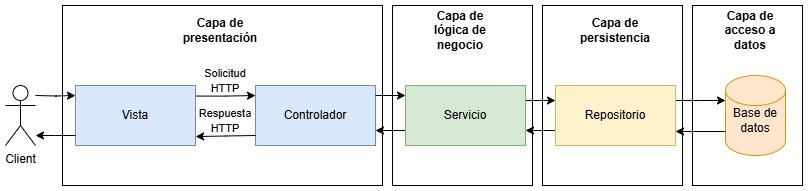
\includegraphics[width=0.95\linewidth]{imagenes/scheme/arquitectura-SIDManager.jpg}
    \caption{Arquitectura de las capas aplicación SIDManager}
    \label{fig:arquitecture_SIDManager}
\end{figure}

\begin{enumerate}
    \item Capa de presentación:
    La capa de presentación es la encargada de manejar la interfaz de usuario y las interacciones del usuario, presentando información a los usuarios y capturando su entrada.
    En este proyecto contiene dos componentes en esta capa, la vista y el controlador.
    Por un lado el cliente accede a las interfaces visuales, las cuales están diseñadas con Thymeleaf para garantizar una generación dinámica y eficiente de las vistas (views). Este motor de plantillas permite incluir datos provenientes del back-end directamente en las páginas HTML, facilitando la comunicación entre ambas capas.
    Por otro lado los controladores (controllers) son responsables de gestionar las peticiones HTTP provenientes del front-end. Estos se encargan de procesar la solicitud y delegar la lógica de negocio al siguiente nivel, los servicios (services). En otras palabras, son conectores que dirigen las peticiones del usuario a los servicios correspondientes sin modificar ni hacer operaciones de lógica de negocio.

    \item Capa de negocio:
    Esta capa es la encargada de implementar la funcionalidad principal y las reglas que impulsan los procesos y operaciones del negocio.
    En la aplicación, está capa esta definida en los servicios, que se encargan de realizar las transformaciones necesarias sobre los datos y delegan las operaciones de almacenamiento o consulta al repositorio.

    \item Capa de persistencia:
    La función principal de esta capa es manejar el almacenamiento y recuperación de datos de bases de datos.
    En este proyecto contiene dos componentes en esta capa, del repositorio y el modelo.
    Por un lado, el repositorio (repository) utiliza JPA (Java Persistence API) y se conecta con la base de datos para realizar operaciones CRUD (Crear, Leer, Actualizar, Eliminar). 
    Por otro lado, el modelo (model) está representado por los datos manejados por la aplicación mediante entidades JPA. Estos modelos mapean las tablas de la base de datos, permitiendo que la lógica de negocio interactúe con ellas de forma directa.
    Esta capa abstrae los detalles de implementación de la base de datos, permitiendo una interacción más sencilla.

    \item Base de datos:
    La función principal de esta capa es almacenar, mantener y administrar datos de forma estructural y organizativa.
    La conexión con la base de datos se realiza mediante JPA, utilizando herramientas ya mencionadas en capítulos anteriores.
\end{enumerate}

Este esquema destaca cómo cada capa cumple un rol específico, asegurando la separación de responsabilidades y facilitando el mantenimiento y escalabilidad del sistema.

Para mayor entendimiento sobre las tecnologías utilizadas en cada capa, se puede ver el esquema de las tecnologías empleadas \ref{fig:technology_arquitecture}.

\begin{figure}
    \centering
    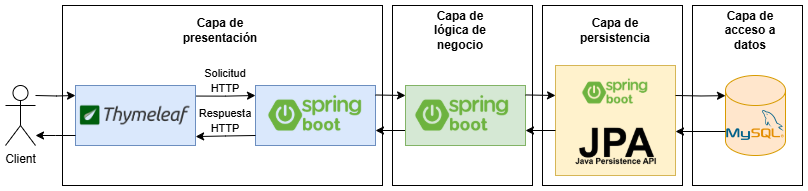
\includegraphics[width=0.95\linewidth]{imagenes//scheme/Tecnologías SIDManager.png}
    \caption{Arquitectura de las tecnologías de la aplicación SIDManager}
    \label{fig:technology_arquitecture}
\end{figure}

\section{Diagrama UML de secuencia}
Antes de desarrollar cualquier proyecto, es fundamental planificar qué se va a implementar y cómo. Por esta razón, mi tutor en la empresa me solicitaba elaborar diagramas de secuencia UML antes de trabajar en funciones clave del sistema. Estos diagramas ayudaban a visualizar el flujo de la aplicación y asegurar un diseño coherente. En este documento, se han incluido dos de los diagramas que se realizaron digitalmente: uno corresponde al proceso de registro (Figura \ref{fig:sign-up-uml-diagram}) y otro al proceso de carga de documentos filtrados por fechas (Figura \ref{fig:list-documents-uml-diagram}).


\begin{figure}
    \centering
    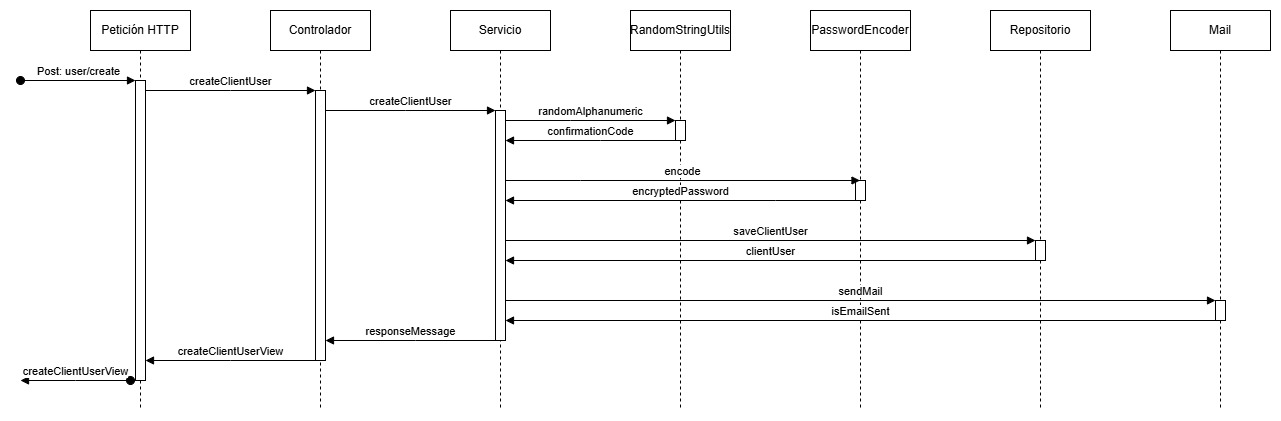
\includegraphics[width=0.95\linewidth]{imagenes/UML/SignUpPostUserCreate.jpg}
    \caption{Diagrama UML de la función createClientUser}
    \label{fig:sign-up-uml-diagram}
\end{figure}

\begin{figure}
    \centering
    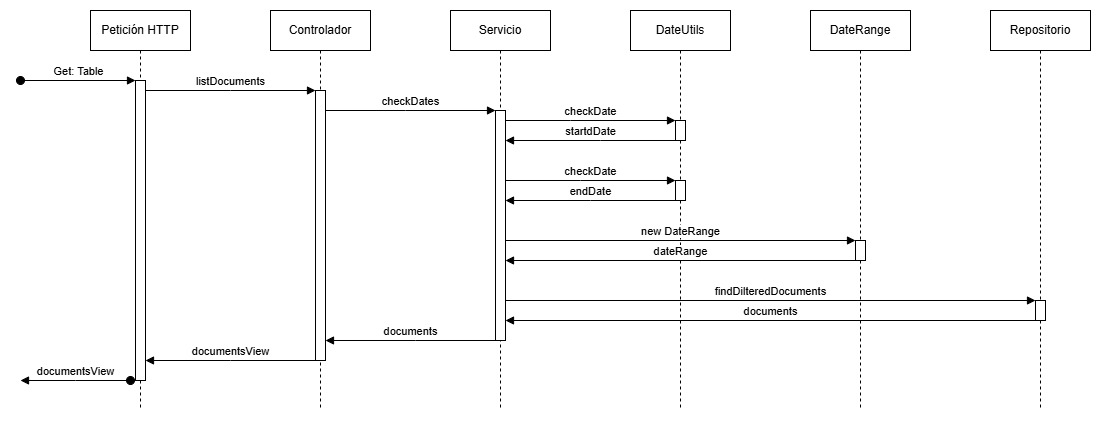
\includegraphics[width=0.95\linewidth]{imagenes/UML/getTable.jpg}
    \caption{Diagrama UML de la función listDocuments}
    \label{fig:list-documents-uml-diagram}
\end{figure}



\section{ Tecnologías selecionadas }

De las opciones de las posibles tecnologías para llevar a cabo el proyecto abordadas en el estado de la cuestión, estas son las que se han elegido:

\subsection{ Spring Boot }
Aunque existen otros frameworks populares hoy en día, como Angular y React, estos están basados en JavaScript, un lenguaje diferente de Java. JavaScript es más versátil al permitir el desarrollo tanto en frontend como en backend, pero presenta desventajas en términos de seguridad. Al no ser un lenguaje tipado ni ejecutarse en una máquina virtual, es más vulnerable a ciertos tipos de ataques, como se explica en el artículo \textcite{java-vs-javascript}. Por esta razón, para este proyecto fue necesario optar por un framework que utilizara Java.

Spring Boot ha sido la tecnología seleccionada para el desarrollo de esta aplicación web debido a sus características que facilitan la creación de aplicaciones empresariales robustas y escalables. 

Dado que el proyecto se centra en la monitorización de documentos en un entorno bancario, donde la seguridad, eficiencia y fiabilidad son aspectos clave, Spring Boot proporciona una base sólida. Con su configuración mínima y capacidades integradas, permite un desarrollo rápido y efectivo, adaptándose a las necesidades de este entorno.

Una de las principales ventajas de Spring Boot es su capacidad para simplificar el desarrollo de aplicaciones complejas gracias a su amplia gama de bibliotecas y configuraciones predeterminadas. Su integración con tecnologías como Spring Security facilita la implementación de controles de acceso y autenticación, esenciales en un entorno bancario. Además, su soporte para la gestión eficiente de bases de datos mediante JPA es ideal para manejar grandes volúmenes de datos, como los documentos almacenados en esta aplicación.

Otra ventaja importante para el uso de Spring Boot es la popularidad de Java, ya que es el séptimo lenguaje de programación más usado por profesionales según \citeauthor{most-used-tech}, como se puede ver en la figura \ref{fig:most-used-tech}. Cabe destacar en popularidad también al propio framework Spring Boot, que es el undécimo framework de desarrollo más utilizado en el mundo, como se muestra en la figura 5.2. Esto garantiza que la tecnología continúe evolucionando, lo que asegura la viabilidad del proyecto a largo plazo, además de la abundante documentación y comunidad de soporte. Spring Boot también es uno de los frameworks preferidos por los bancos, como se destaca en distintos artículos online como \textcite{java-usage-banks}. Esto se debe a su robustez, estabilidad, seguridad y escalabilidad, características clave en aplicaciones empresariales críticas.

\begin{figure}
    \centering
    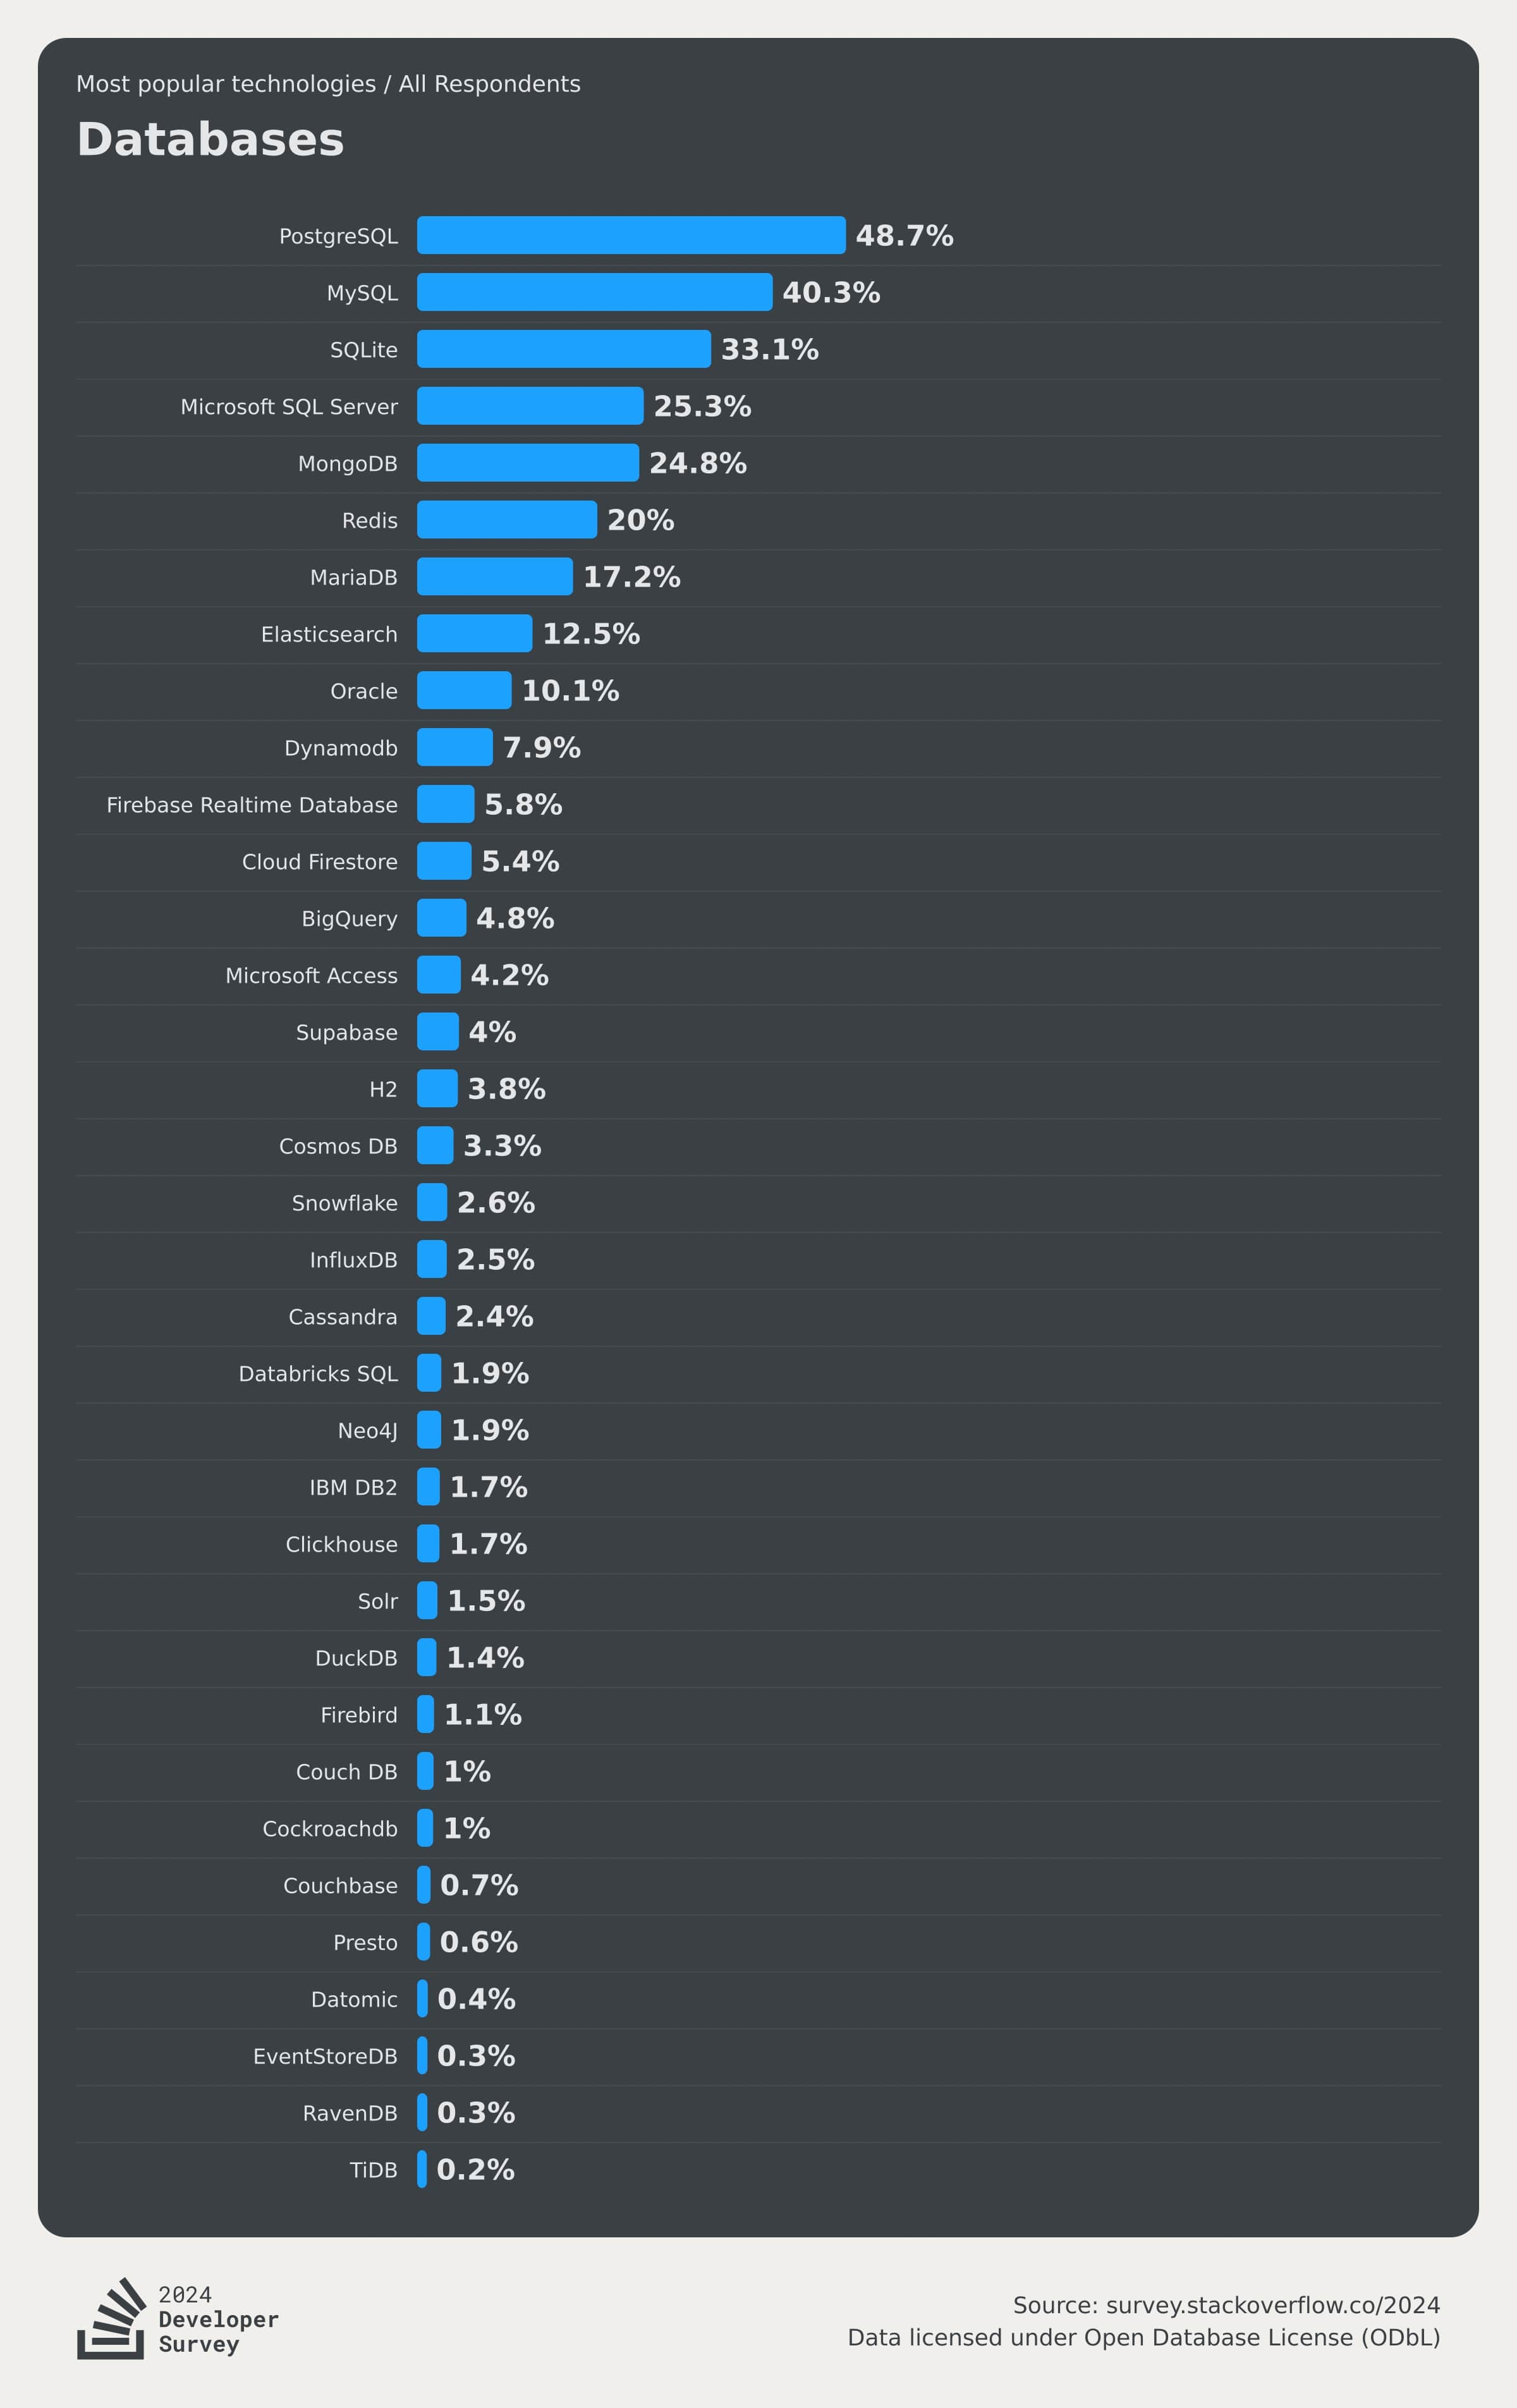
\includegraphics[width=0.85\linewidth]{imagenes/charts/java_stadistics.jpg}
    \caption{Gráfico de tecnologías más populares. Fuente: \textcite{most-used-tech}.}
    \label{fig:most-used-tech}
\end{figure}

\begin{figure}
    \centering
    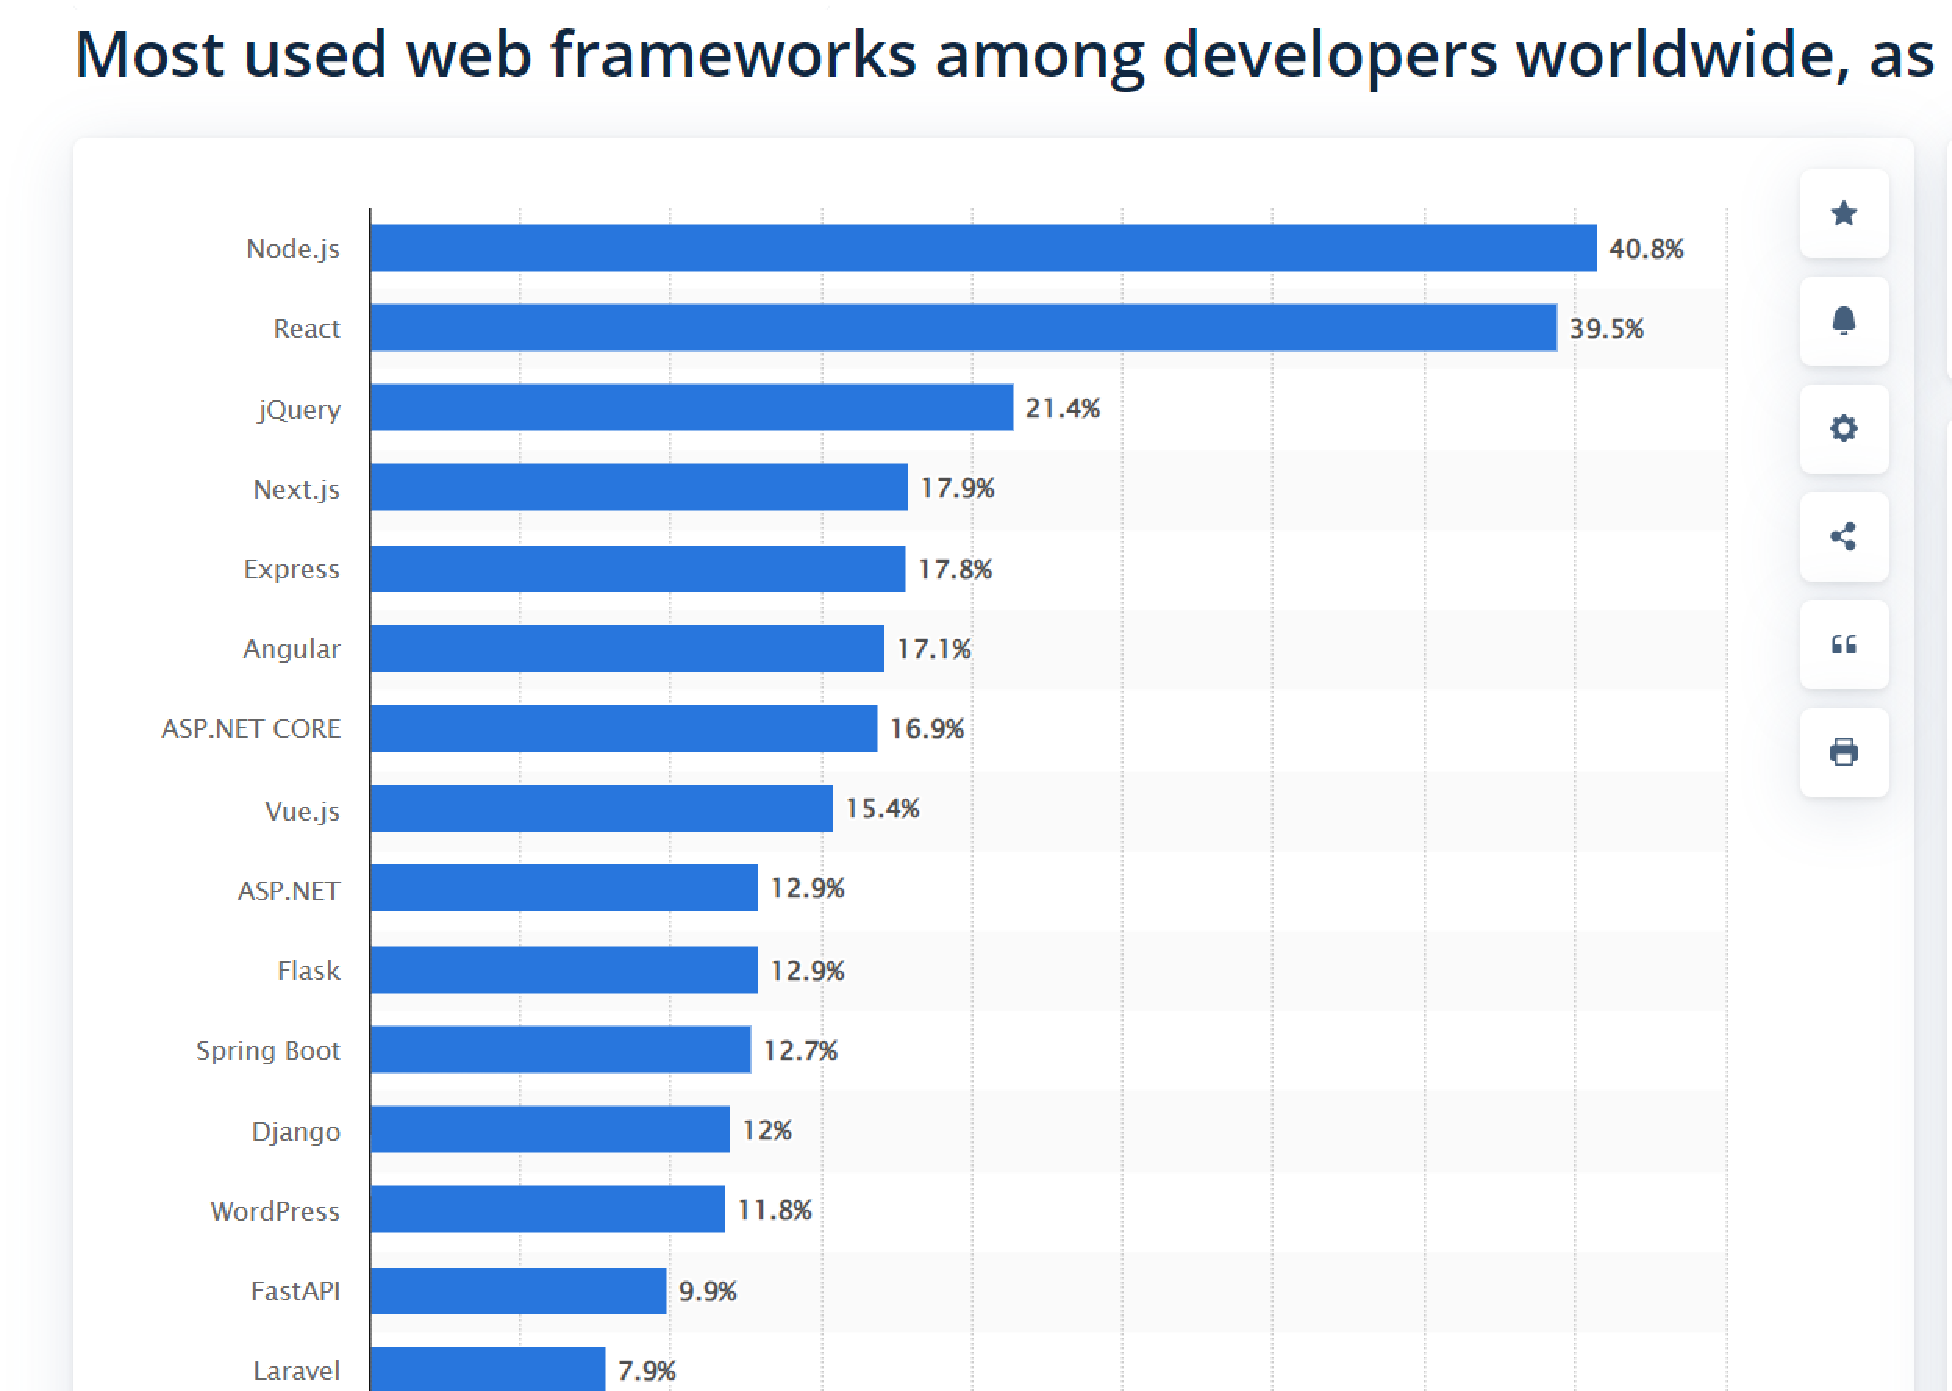
\includegraphics[width=0.9\linewidth]{imagenes/charts/spring_boot_stadistics.pdf}
    \caption{Gráfico de frameworks web más usados por desarrolladores. Fuente: \textcite{most-used-frameworks}.}
    \label{fig:most-used-frameworks}
\end{figure}



No obstante, el uso de Spring Boot también presenta ciertos inconvenientes. Aunque su automatización y configuraciones predeterminadas aceleran el desarrollo, en proyectos a gran escala pueden generar una sobrecarga del sistema si no se optimizan los recursos adecuadamente. La facilidad para incluir dependencias adicionales puede aumentar la complejidad del proyecto, afectando al rendimiento y a la mantenibilidad del código a largo plazo.

Otro aspecto a considerar es que, al estar basado en Java, Spring Boot puede requerir mayores recursos de memoria y procesamiento en comparación con tecnologías más ligeras. Esto puede ser un reto en servidores con limitaciones de hardware o cuando se buscan optimizaciones de recursos.

A pesar de estos inconvenientes, Spring Boot sigue siendo una opción sólida y flexible para desarrollar aplicaciones empresariales seguras y escalables, como es el caso de esta solución para la gestión documental en entornos bancarios.

\subsection{ Maven }

Maven ha sido elegido como la herramienta de gestión de dependencias y automatización de la construcción para este proyecto debido a su fiabilidad y popularidad en el ecosistema Java. Una de las principales razones por las que Maven es ampliamente utilizado en proyectos empresariales es su capacidad para simplificar la gestión de dependencias, lo que facilita la integración de bibliotecas externas necesarias para el correcto funcionamiento de la aplicación.

Una ventaja significativa de Maven es su capacidad para gestionar de manera eficiente las versiones de las dependencias y sus transitorios, asegurando que siempre se utilicen versiones compatibles y actualizadas de las bibliotecas, lo que es crucial para mantener la seguridad y estabilidad del proyecto en el tiempo. Además, Maven proporciona una estructura de proyecto estándar y bien organizada, lo que facilita la colaboración entre distintos equipos y la integración con herramientas de \acrfull{cicd}.

Según la encuesta de Stack Overflow, Maven es una de las herramientas de automatización de construcción más usadas en el mundo, lo que garantiza una amplia documentación y soporte por parte de la comunidad, como muestran los informes de \textcite{most-used-tech}. Esto asegura la viabilidad de su uso a largo plazo, además de la fácil capacitación de nuevos desarrolladores que se unan al proyecto.

Sin embargo, uno de los inconvenientes de Maven es su curva de aprendizaje inicial, especialmente para desarrolladores que no están familiarizados con su configuración basada en XML. Además, en proyectos de gran escala, la acumulación de dependencias puede generar archivos de configuración extensos y difíciles de manejar si no se estructuran adecuadamente. Otro aspecto a considerar es el tiempo de compilación, que puede ser considerable en proyectos grandes debido a la resolución de dependencias y la construcción de los módulos.

A pesar de estos inconvenientes, Maven sigue siendo la opción ideal para este proyecto, ya que proporciona una solución integral para la gestión de dependencias y la automatización de la construcción, permitiendo un desarrollo ágil y organizado.

\subsection{ Thymeleaf }

Thymeleaf ha sido seleccionado como el motor de plantillas para el desarrollo del frontend de esta aplicación debido a su estrecha integración con Spring Boot y su capacidad para crear vistas dinámicas basadas en HTML. Al ser una tecnología diseñada específicamente para aplicaciones web Java, Thymeleaf permite renderizar páginas de manera eficiente, con una sintaxis que resulta intuitiva para los desarrolladores que ya están familiarizados con HTML y CSS.

Una de las principales ventajas de Thymeleaf es que permite construir plantillas que son directamente visualizables en navegadores, incluso sin un servidor backend activo, lo que agiliza el desarrollo de interfaces. Esto se alinea con la necesidad de este proyecto de desarrollar una aplicación web accesible y fácil de mantener. Además, Thymeleaf soporta la validación de formularios y la internacionalización, características clave para una aplicación que pueda ser utilizada en distintos contextos empresariales y por usuarios de diversas regiones.

Según la propia web de \citeauthor{thymeleaf-downloads}, es uno de los motores de plantillas más populares dentro del ecosistema de Spring, ya que tiene más de un millón y medio de descargas al mes, lo que asegura la existencia de abundante documentación y ejemplos prácticos, como se puede ver en el siguiente gráfico \ref{fig:descargas_mensuales_thymeleaf}. Esto facilita su integración y reduce la curva de aprendizaje para nuevos desarrolladores.

\begin{figure}
    \centering
    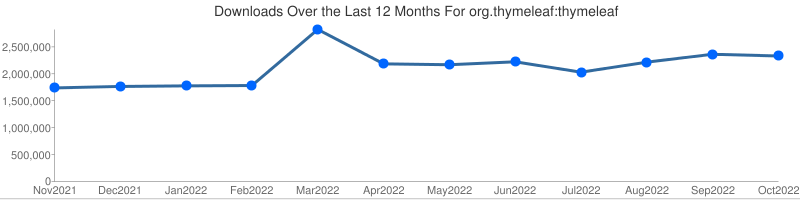
\includegraphics[width=0.75\linewidth]{imagenes/charts/thymeleaf_usage.png}
    \caption{Descargas mensuales de Thymeleaf. Fuente: \textcite{thymeleaf-downloads}.}
    \label{fig:descargas_mensuales_thymeleaf}
\end{figure}

No obstante, Thymeleaf presenta algunos inconvenientes. Al ser un motor de plantillas del lado del servidor, puede tener un rendimiento inferior en comparación con soluciones de frontend basadas en JavaScript, como React o Angular, especialmente cuando se trata de aplicaciones con una gran cantidad de interacciones simultáneas. Además, la generación de vistas en el servidor puede aumentar la carga de procesamiento en aplicaciones con un gran número de usuarios concurrentes, lo que puede requerir optimizaciones adicionales en el backend.

A pesar de estos desafíos, Thymeleaf sigue siendo una opción adecuada para este proyecto, ya que facilita la creación de una interfaz de usuario dinámica y bien integrada con Spring Boot, manteniendo un enfoque en la simplicidad y la seguridad, lo cual es crucial para aplicaciones bancarias y empresariales.


\subsection{ JPA }

JPA (Java Persistence API) ha sido elegido en este proyecto por su capacidad para simplificar la interacción con la base de datos, eliminando la necesidad de escribir consultas SQL manuales en la mayoría de los casos. Al trabajar con JPA, el desarrollador puede centrarse en los objetos de dominio de Java, ya que JPA se encarga de la persistencia de los datos de manera automática, permitiendo asignar las entidades directamente a las tablas de la base de datos.

Una de las principales ventajas de JPA es su capacidad para abstraer la complejidad del SQL. Esto simplifica el desarrollo al utilizar operaciones CRUD predefinidas y un lenguaje de consultas más amigable como \acrfull{jpql}, que evita la necesidad de escribir SQL detallado. Además, JPA se integra perfectamente con Spring Data, lo que permite generar repositorios y consultas dinámicas de forma automática, lo cual mejora la productividad y reduce el riesgo de errores en la interacción con la base de datos.

\begin{figure}
    \centering
    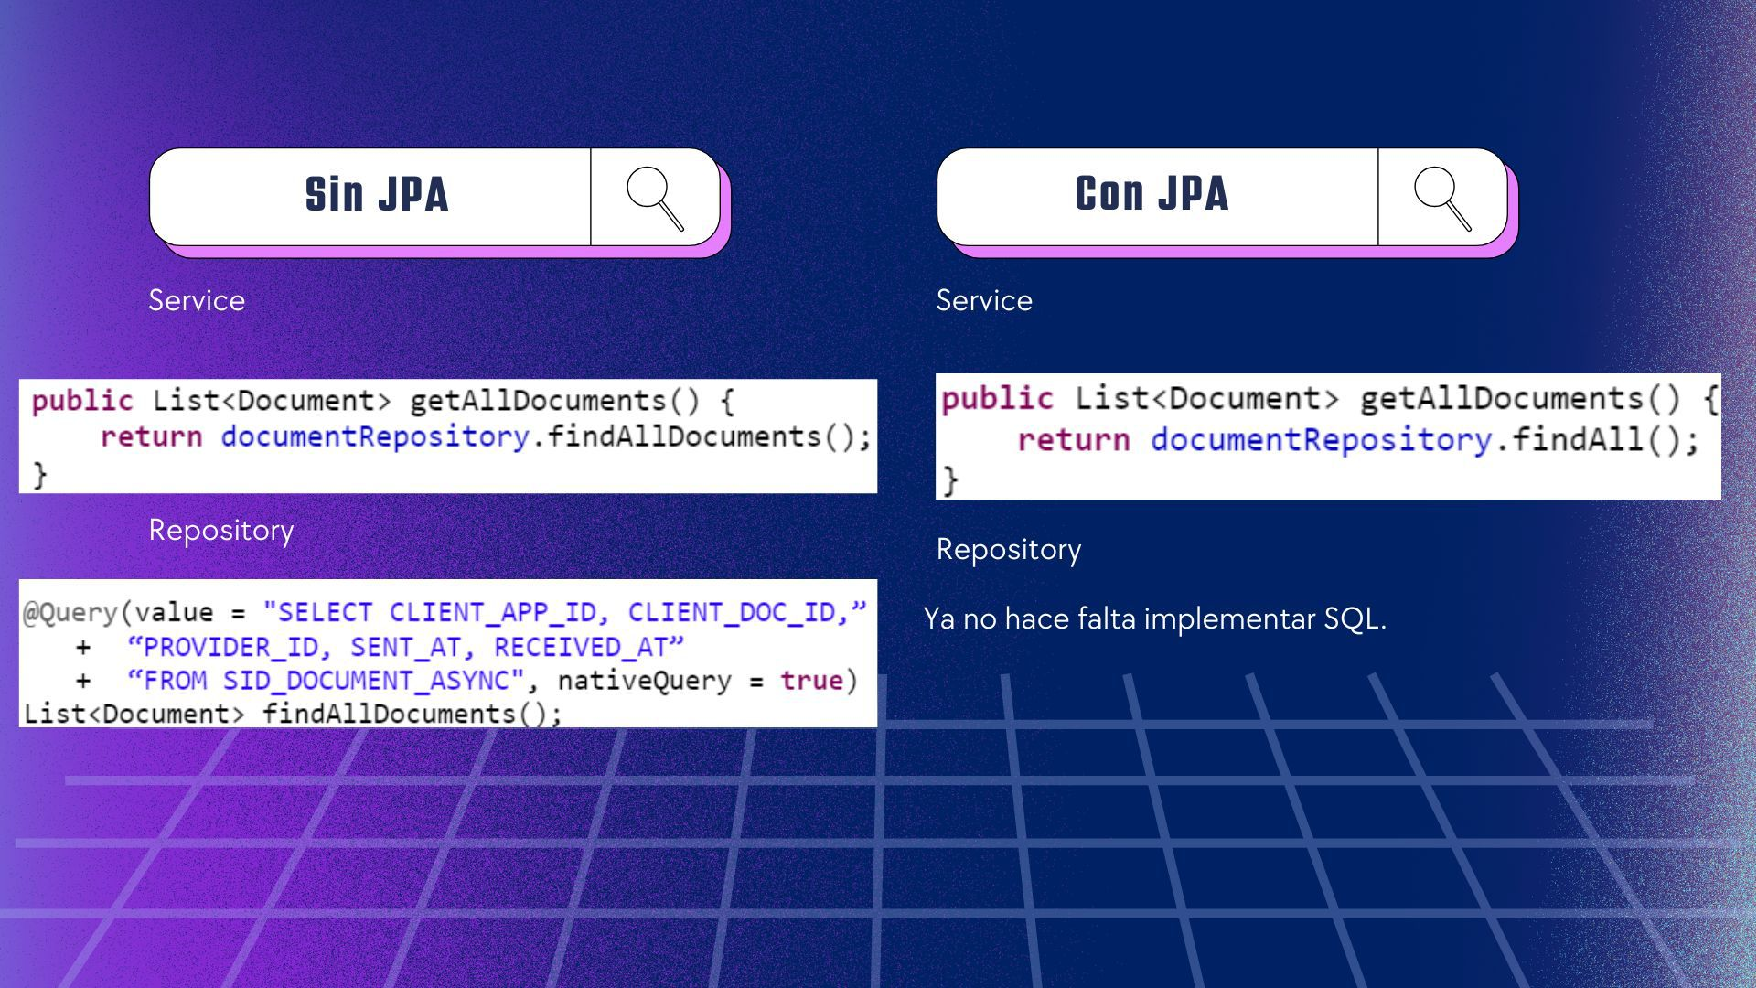
\includegraphics[width=0.75\linewidth]{imagenes/code/JPA_usage.pdf}
    \caption{Diferencia entre usar y no usar JPA (elaboración propia).}
    \label{fig:jpa-usage}
\end{figure}

JPA también garantiza la independencia de la base de datos, ya que facilita la migración entre distintos sistemas de gestión de bases de datos sin cambios significativos en el código. 

Sin embargo, uno de los inconvenientes de JPA es su rendimiento en escenarios con consultas SQL muy complejas o específicas, donde puede ser necesario optimizar manualmente el SQL para obtener mejores tiempos de respuesta. Además, JPA puede añadir una cierta sobrecarga en términos de recursos debido a la gestión de la caché y las transacciones automáticas.

A pesar de estos desafíos, JPA sigue siendo una opción ideal para este proyecto, ya que facilita enormemente la gestión de la persistencia de datos, minimizando la necesidad de escribir SQL manual y aumentando la eficiencia del desarrollo.

%% \chapter{Implementación} \label{implementacion}

% En este capítulo, se va a describir detalladamente la implementación de este proyecto. Primeramente, definiremos el entorno de desarrollo para más adelante poder abordar la implementación de la API, la implementación del acceso a la base de datos, la implementación de funcionalidades avanzadas de Spring Boot, la implementación del login, la implementación de la vista con Thymeleaf y, por último, las funcionalidades extras que hacen del proyecto una aplicación altamente versátil.

% \section{Entorno de desarrollo}

% El entorno de desarrollo utilizado para este proyecto se basa en un equipo portátil con las siguientes características técnicas:

% \begin{itemize}
%     \item Sistema operativo: Windows 11.
%     \item Memoria \acrshort{ram}: 16 \acrshort{gb}.
%     \item Procesador: Intel Core i7.
% \end{itemize}


% Esta configuración ha permitido un rendimiento fluido durante las distintas etapas del desarrollo, desde la programación hasta las pruebas de la aplicación, por lo que el uso de un dispositivo de características similares para recrear el proyecto sería más que suficiente.

% Para la implementación del sistema, se ha utilizado el entorno de desarrollo integrado (o \acrshort{ide}) Eclipse, versión 4.28.0. Eclipse es ampliamente reconocido por su soporte robusto para proyectos Java y su integración con herramientas como Maven, facilitando la gestión de dependencias y el ciclo de vida del proyecto, como se ha explicado anteriormente.

% El proyecto se ha desarrollado utilizando el marco de trabajo Java Spring Boot en su versión 2.7.18. Recordemos que Spring Boot es una herramienta poderosa para la creación de aplicaciones Java empresariales, ya que simplifica la configuración inicial y proporciona una estructura robusta para aplicaciones web.

% El lenguaje de programación empleado ha sido Java, utilizando el \acrfull{jdk} 1.8. Este entorno de ejecución permite una amplia compatibilidad con bibliotecas y herramientas esenciales para el desarrollo.

% Para la gestión de dependencias, compilación y empaquetado del proyecto, se ha utilizado Apache Maven en su versión 4.0.0. Maven permite gestionar las bibliotecas externas de manera eficiente, garantizando que todas las dependencias estén sincronizadas y disponibles en las versiones correctas. Esto se configura a través del archivo `pom.xml`, que define las dependencias necesarias y sus versiones, como se puede ver en la Figura \ref{fig:maven_pom}.

% \begin{figure}
%     \centering
%     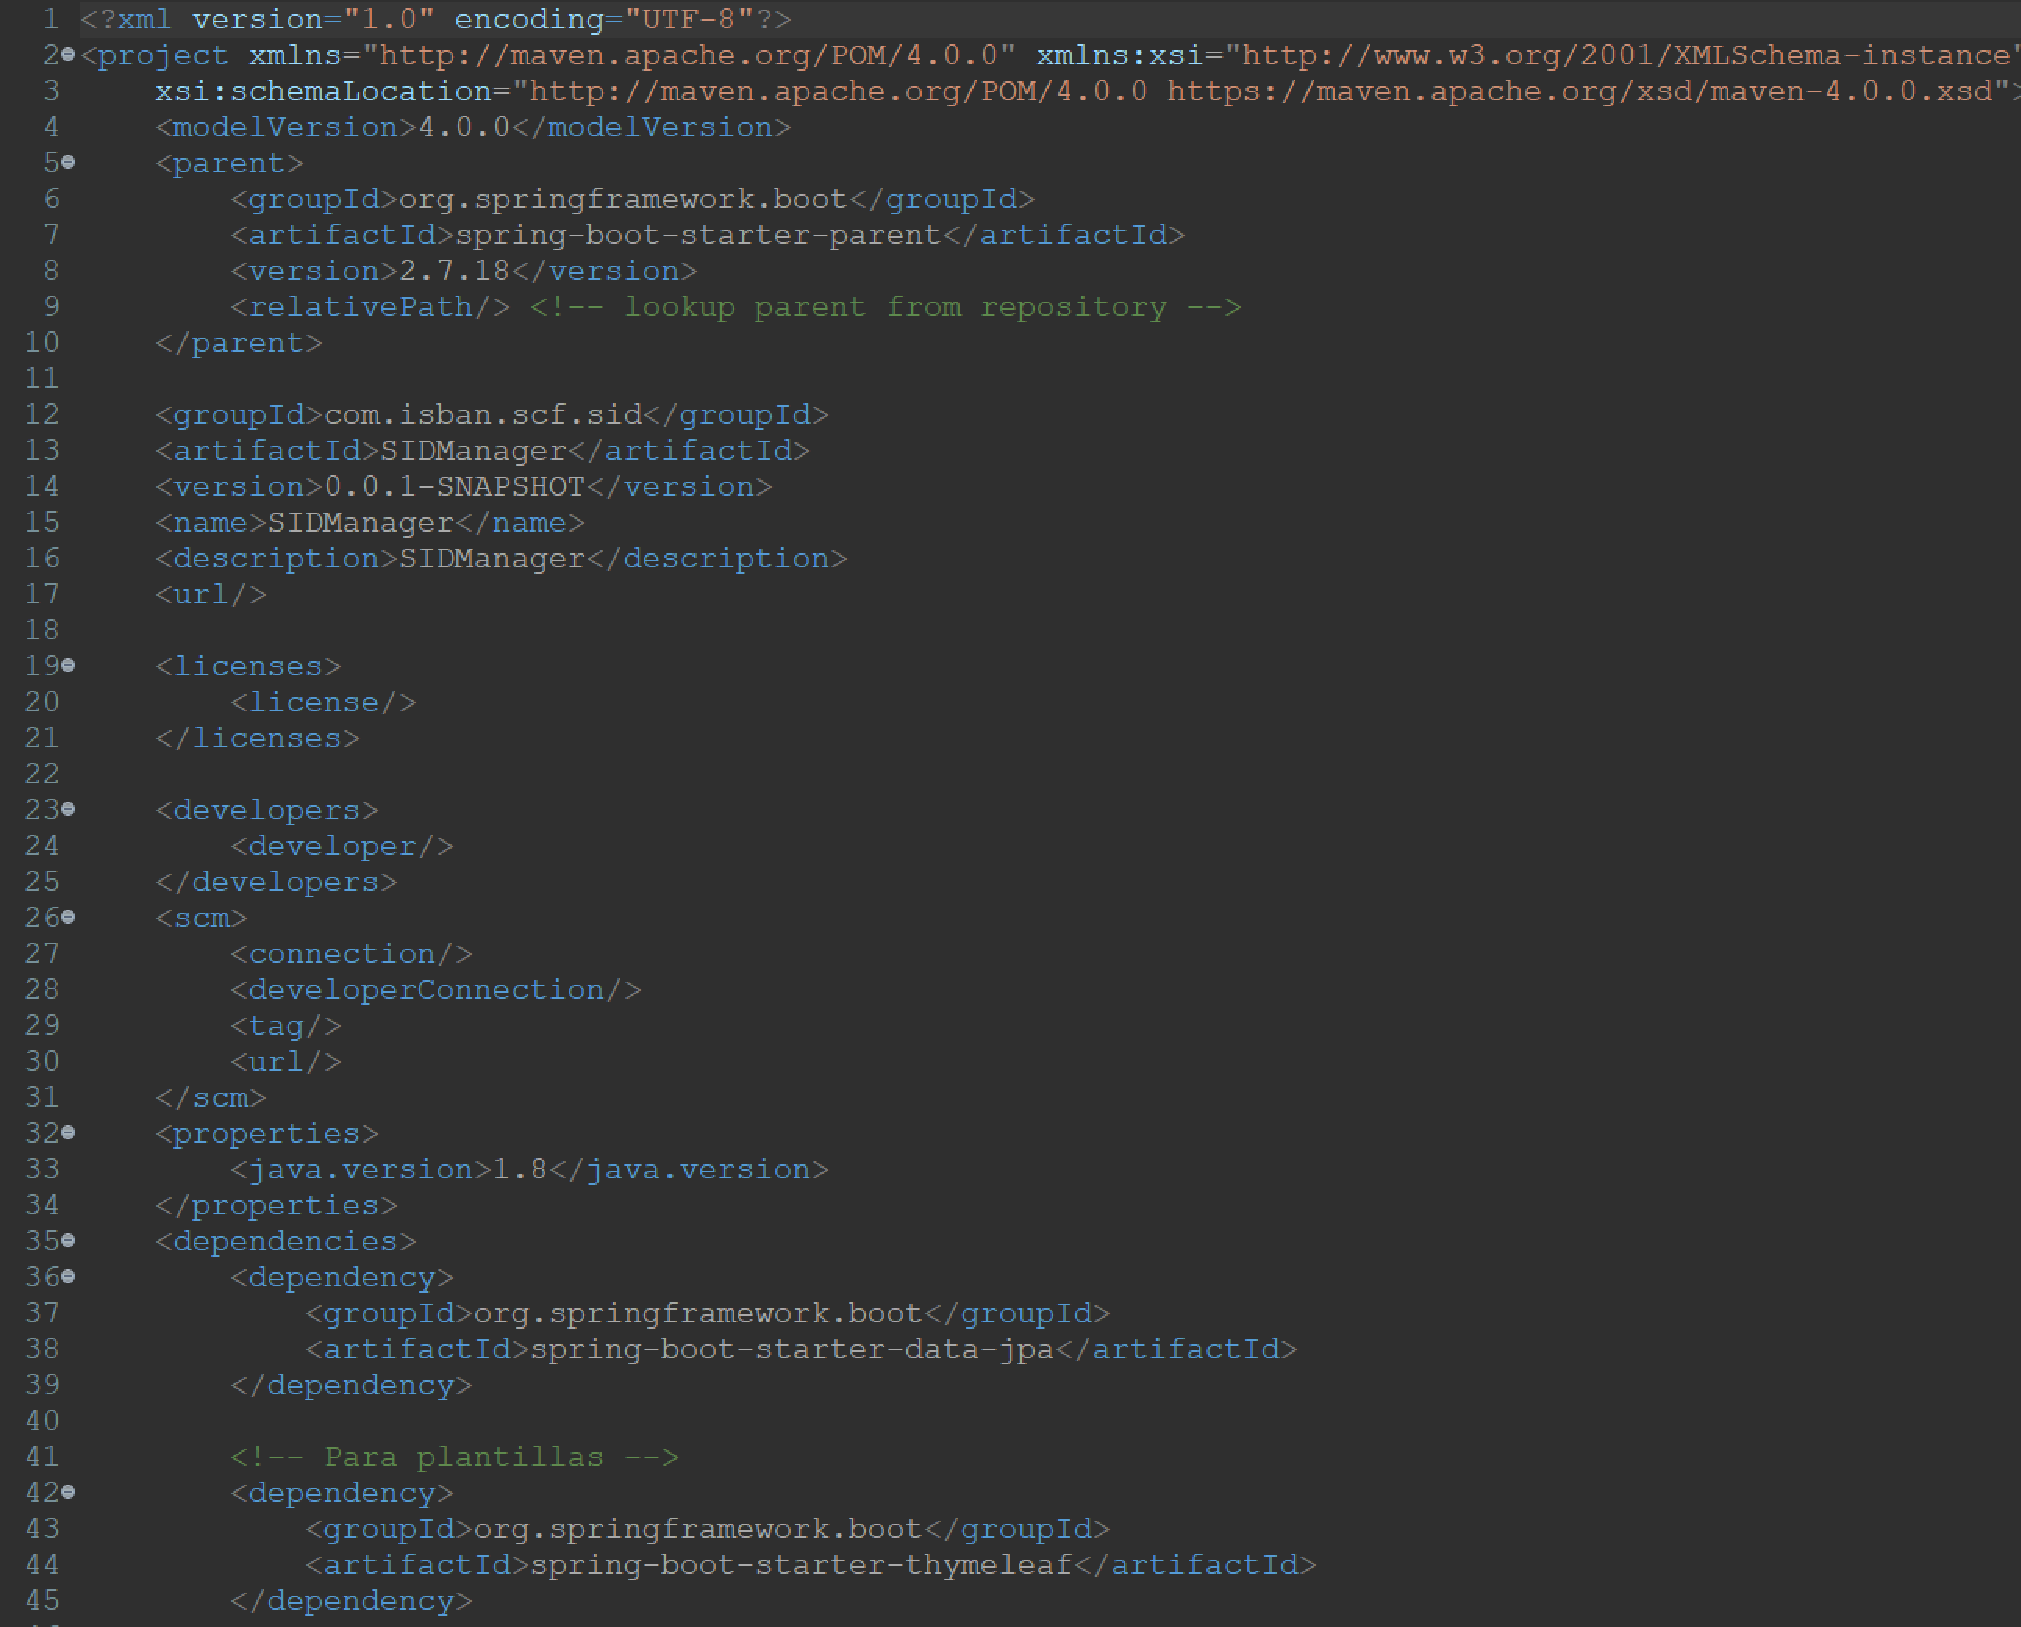
\includegraphics[width=0.75\linewidth]{imagenes/code/maven_pom_xml_example.pdf}
%     \caption{Archivo pom.xml de Maven del proyecto}
%     \label{fig:maven_pom}
% \end{figure}

% \subsection{Dependencias principales}

% A continuación, se describen las principales dependencias empleadas en el proyecto y su propósito:

% \begin{enumerate}
%     \item Thymeleaf:
%     Es un motor de plantillas que permite integrar datos dinámicos en las vistas HTML. Para más información, lea el apartado \ref{subsec:thymeleaf}.

%     \item MySQL Connector:
%     Este conector es la biblioteca que permite la conexión entre la aplicación Java y la base de datos MySQL. Es fundamental para realizar operaciones de consulta, inserción, actualización y eliminación en la base de datos.

%     \item javax.mail:
%     Biblioteca utilizada para la implementación de funcionalidades de envío de correos electrónicos. En este proyecto, se emplea para enviar correos de confirmación a los usuarios registrados, asegurando una validación adecuada de sus cuentas.

%     \item Javadoc:
%     Javadoc es una herramienta incluida en el JDK que permite generar documentación de las clases y métodos del proyecto a partir de comentarios en el código fuente. Esto facilita la comprensión y el mantenimiento del sistema.

%     \item Log4j:
%     Log4j es una biblioteca para la gestión de bitácoras (logs). Se utiliza para registrar eventos, errores y mensajes informativos durante la ejecución de la aplicación, lo que es crucial para la depuración y monitorización.

% \end{enumerate}



% \section{ API de gestión de documentos}

% Para poder hablar de la API, es importante hacer una distinción entre las dos partes principales de la aplicación: por un lado, la gestión de documentos, y por otro, la gestión de usuarios.

% En este apartado, se va a hablar de la gestión de documentos, es decir, de cómo funciona la aplicación por dentro para mostrar por pantalla el listado con las características de los documentos.

% Encontramos tres funciones principales en el controlador: getAllDocuments, getNotReceivedDocuments y listDocuments.


% \subsection{ Función getAllDocuments }
% Esta función llama al método \emph{getAllDocuments} del servicio \emph{DocumentService} y devuelve la respuesta. El código de la función \emph{getAllDocuments}, junto con sus logs asociados, es el siguiente:

% \begin{lstlisting}[language=Java]
% @GetMapping()
% public String getAllDocuments(Model model) {
%     logger.debug(" ----- Entering getAllDocuments ----- ");
%     model.addAttribute("documents", documentService.getAllDocuments());
%     logger.debug(" ----- Exiting getAllDocuments ----- ");
%     logger.debug(" ____________________________________ ");
%     return "documentsView"; 
% }
% \end{lstlisting}

% Una vez en el método \emph{getAllDocuments} del \emph{DocumentService}, este llama a la función \emph{findAll} del \emph{DocumentRepository}, que es el repositorio encargado de interactuar con la base de datos. El código es el siguiente:

% \begin{lstlisting}[language=Java]
% public List<Document> getAllDocuments() {
%     logger.debug(" Entering findAllDocuments ");
%     return documentRepository.findAll();
% }
% \end{lstlisting}

% Gracias a JPA, la sintaxis utilizada (\emph{findAll}) permite generar automáticamente la consulta SQL sin necesidad de que el programador escriba la consulta explícitamente en el \emph{DocumentRepository}. Esto no solo ahorra tiempo, sino que también reduce la posibilidad de errores y mejora la claridad del código. Para una mejor comprensión, se recomienda revisar la figura \ref{fig:jpa-usage}.

% Más adelante, en la sección \ref{sec:jpa-sintaxis}, se explicará con más detalle el uso de JPA.

% En resumen, esta función devuelve todos los documentos de la base de datos, sin restricciones ni filtros aplicados, junto con sus respectivos datos asociados (tal como se explicó en la sección de arquitectura de los documentos \ref{subsec:document-architecture}).

    
% \textbf { \subsection { Función getNotReceivedDocuments }}
%     Esta función llama al método \emph{getNotReceivedDocuments} del servicio \emph{DocumentService} y devuelve la respuesta. El código de la función \emph{getNotReceivedDocuments}, junto con sus logs asociados, se puede observar en el anexo \ref{code:not-received-controller}.

% Una vez en el método \emph{getNotReceivedDocuments} del \emph{DocumentService}, este llama a la función \emph{findByReceivedAtIsNull} del \emph{DocumentRepository}. El código se puede observar en el anexo \ref{code:not-received-service}.



% En resumen, esta función devuelve todos los documentos de la base de datos que no hayan sido guardados correctamente, ya que no tienen fecha en el apartado \emph{received\_at} (para más información sobre la arquitectura del documento, ver la sección \ref{subsec:document-architecture}), por lo que no han sido recibidos. 

    
%     \textbf { \subsection { Función listDocuments}}

% La función \emph{listDocuments} es una de las piezas clave de la aplicación, ya que se encarga de recuperar y filtrar los documentos almacenados en la base de datos según un intervalo de fechas. Esta función combina dos métodos principales del servicio \emph{DocumentService}: \emph{checkDates} y \emph{getFilteredDocuments}. Para una primera comprensión de la función, se puede visualizar el diagrama de secuencia UML del apartado de diseño \ref{fig:list-documents-uml-diagram}. A continuación, se describe en detalle su funcionamiento y los componentes involucrados.


% La función \emph{listDocuments} realiza principalmente tres tareas: validación y ajuste de fecha, filtrado de documentos y preparación de la respuesta.
% A través del método \emph{checkDates}, se valida y ajusta el intervalo de fechas proporcionado por el usuario. Este intervalo se almacena en una clase auxiliar llamada \emph{DateRange}, que encapsula las fechas de inicio y fin para facilitar su manejo entre métodos.
% Utilizando el intervalo de fechas validado, se invoca el método \emph{getFilteredDocuments} para recuperar los documentos que cumplen con el criterio de filtrado.
% Finalmente, la función añade al modelo (\emph{model}) los documentos filtrados, junto con las fechas de inicio y fin utilizadas en el filtrado. Esta información se envía a la vista para su visualización.


% El código de la función \emph{listDocuments}, junto con sus logs asociados, se puede apreciar en el anexo \ref{code:list-docs}.


% Una vez que el intervalo de fechas ha sido validado, la función \emph{listDocuments} invoca el método \emph{getFilteredDocuments} del servicio \emph{DocumentService}. Este método, a su vez, llama a una función del repositorio \emph{DocumentRepository} para ejecutar la consulta SQL que filtra los documentos según las fechas proporcionadas. Se puede consultar el código en el anexo \ref{code:list-docs-service}.


% Dado que esta consulta es específica y no se ajusta a las convenciones automáticas de JPA, se ha implementado manualmente en el repositorio utilizando una anotación \emph{@Query}. La consulta SQL correspondiente se puede ver en el código del repositorio que está en el anexo \ref{code:list-docs-repositoty}.



% Método \emph{checkDates}

% El método \emph{checkDates} desempeña un papel crucial en la función \emph{listDocuments}, ya que se encarga de validar y ajustar las fechas proporcionadas por el usuario. Su implementación responde a tres necesidades principales: validación de errores, pseudopaginación y manejo de casos especiales.
% Respecto a la validación de errores, esta garantiza que las fechas proporcionadas sean válidas y estén en el formato correcto. Si no se realiza esta validación, errores en las fechas podrían interrumpir el funcionamiento de la aplicación.
% Por otro lado, en entornos de preproducción, se observó que la carga de más de 80.000 documentos podía tardar entre 6 y 8 minutos. Para optimizar el rendimiento, se implementó una pseudopaginación que limita el intervalo de fechas a un máximo de 10 días. Este límite se estableció tras un análisis exhaustivo que demostró que, a partir de este número, el tiempo de carga comenzaba a ser demasiado largo (3 segundos).
% Finalmente, el método gestiona situaciones en las que el usuario no proporciona ambas fechas o cuando el intervalo de fechas excede el límite establecido; en este caso, el límite es de 10 días como se ha comentado anteriormente.

% El código del método \emph{checkDates} se puede apreciar en el anexo \ref{code:checkDates}.



% El método \emph{checkDates} está diseñado para manejar cinco escenarios principales:

% \begin{itemize}
%     \item Ambas fechas proporcionadas: Si las fechas son válidas y el intervalo no excede los 10 días, se devuelve el intervalo original. En caso contrario, se ajusta el intervalo a los últimos 10 días y se notifica al usuario.
    
%     \item Solo la fecha de fin proporcionada: Se calcula un intervalo de 10 días hacia atrás a partir de la fecha de fin.
    
%     \item Solo la fecha de inicio proporcionada: Se calcula un intervalo de 10 días hacia adelante a partir de la fecha de inicio.
    
%     \item Ninguna fecha proporcionada: Se devuelve un intervalo predeterminado de los últimos 10 días.
    
%     \item Error en el formato de las fechas: Si ocurre un error al parsear las fechas, se devuelve un intervalo predeterminado y se registra el error.
% \end{itemize}


% En resumen, la función \emph{listDocuments} permite recuperar documentos filtrados por un intervalo de fechas, optimizando el rendimiento mediante la pseudopaginación y garantizando la robustez del sistema mediante la validación de entradas. Este enfoque no solo mejora la experiencia del usuario, sino que también asegura un manejo eficiente de grandes volúmenes de datos.


% \section{ API de gestión de usuarios}
% En lo que respecta a la gestión de usuarios, encontramos tres apartados principales (proceso de registro, inicio de sesión y cambio de contraseña) en los que se agrupan las distintas funciones del controlador ClientController. Estos apartados son: registro de usuarios, inicio de sesión y cambio de contraseña.

% % Sign Up
%  \subsection{ Registro de usuarios (signup) }
% El proceso de registro en la aplicación SIDManager consta de tres pasos (o funciones). El primero es la carga de la página de registro, el segundo es el proceso de registrarse y el tercero es la confirmación del usuario a través del correo electrónico. Estos tres pasos se corresponden a tres funciones distintas: getCreateClientUserView, createClientUser, getConfirmation. Las funciones están detalladas a continuación:


% \begin{enumerate}
%     \item  Función getCreateClientUserView

    
%     Esta función devuelve la vista (o página) del proceso de registro del usuario. La función en el ClientController se encuentra en el anexo \ref{code:getCreateClientUserView}.

%     Esta función devuelve la vista ante la petición GET del usuario para poder comenzar el registro. Después de rellenar los campos del registro (correo electrónico, contraseña y contraseña repetida) con los datos del usuario y de pulsar el botón "sign up" se llama a la función createClientUser.
    

%   \item  Función createClientUser

% La función \emph{createClientUser} es la encargada de gestionar el proceso de registro de un nuevo usuario en la aplicación. Esta función recibe los datos del formulario de registro, valida la información y, si todo es correcto, guarda al usuario en la base de datos y envía un correo electrónico de confirmación. Para una primera comprensión de la función, se puede visualizar el diagrama de secuencia UML del apartado de diseño \ref{fig:sign-up-uml-diagram}. Para ver el código, consulta el anexo \ref{code:createClientUser-controller}.


% Los parámetros de entrada son los siguientes:
%     \begin{itemize}
%         \item \emph{Model model}: Se utiliza para pasar datos a la vista, como mensajes de respuesta o errores.
%         \item \emph{@ModelAttribute ClientUser clientUser}: Contiene los datos del usuario proporcionados en el formulario de registro (correo electrónico y contraseña).
%         \item \emph{@RequestParam("psw-repeat") String passwordRepeat}: Contiene la contraseña repetida para verificar que coincida con la contraseña original.
%     \end{itemize}

%     Lógica del controlador:
%     La función llama al método \emph{createClientUser} del servicio \emph{ClientUserService}, pasando los datos del usuario y la contraseña repetida.
%     Dependiendo del resultado del servicio, se añade un mensaje de respuesta al modelo (\emph{model}) para informar al usuario sobre el éxito o el fracaso del registro.
%     Finalmente, se devuelve la vista \emph{createClientUserView}, que muestra el formulario de registro junto con el mensaje de respuesta.


%      \item  Función \emph{saveClientUser}

% La función \emph{saveClientUser} es la encargada de guardar un nuevo usuario en la base de datos. Esta función realiza varias operaciones críticas, como la encriptación de la contraseña, la generación de un código de confirmación único y la asignación de un estado inicial al usuario. Se puede ver la función en el anexo \ref{code:saveClientUser-controller}.

%     En primer lugar, la contraseña proporcionada por el usuario se encripta utilizando la función \emph{encryptFacade}. Esto garantiza que la contraseña no se almacene en texto plano en la base de datos, mejorando la seguridad del sistema. Para más información sobre la encriptación, ver la sección \ref{sec:cryptography}.

%     Por otro lado, se genera un código de confirmación único utilizando \emph{RandomStringUtils.randomAlphanumeric(30)}. Este código se enviará al usuario por correo electrónico y se utilizará para confirmar su registro.

%     Además de lo anterior, el estado del usuario se establece en \emph{0}, lo que indica que el usuario ha sido creado pero aún no ha confirmado su correo electrónico. Mientras tenga su estado en 0, no podrá iniciar sesión, por lo que tendrá que confirmar al usuario abriendo el correo con el enlace proporcionado para ello.

%     También se registra la fecha y hora actuales como la fecha de creación del usuario.

%     Finalmente, el usuario se guarda en la base de datos utilizando el método \emph{save} del repositorio \emph{clientUserRepository}.

%     Si ocurre algún error durante el proceso (por ejemplo, si la contraseña es nula), se lanza una excepción y se registra el error en los logs.

% Las funciones explicadas anteriormente trabajan juntas para garantizar un proceso de registro seguro y eficiente.
% Primeramente, respecto a la validación de datos, la función \emph{createClientUser} valida que las contraseñas coincidan y que el correo electrónico no esté ya registrado en la base de datos.
% Además de lo anterior, la función \emph{saveClientUser} se encarga de encriptar la contraseña, generar un código de confirmación único y guardar al usuario en la base de datos.
% Una vez que el usuario se ha guardado correctamente, se envía un correo electrónico con el código de confirmación para que el usuario pueda activar su cuenta.
% Para finalizar, el controlador devuelve un mensaje de respuesta a la vista, informando al usuario sobre el éxito o el fracaso del registro.
    

% Las funciones comentadas son fundamentales para el proceso de registro en la aplicación SIDManager. Juntas, garantizan que los datos del usuario se validen, almacenen de manera segura y se confirmen a través de un correo electrónico. Este enfoque no solo mejora la seguridad del sistema, sino que también proporciona una experiencia de usuario fluida y confiable.
    
%     \item Función getConfirmation

% Antes de explicar la función \emph{getConfirmation}, es importante recordar que un usuario, al crearse, tiene un estado inicial de \emph{0} (creado pero no confirmado). Para confirmar su cuenta, se le envía un correo electrónico con un enlace único que lo redirige a una página de confirmación. Esta página cambia su estado a \emph{1} (confirmado) una vez que el usuario accede al enlace. La función \emph{getConfirmation} en el \emph{UserController} es la encargada de gestionar este proceso. Para ver el código de la función, consultar \ref{code:getConfirmation-controller}.


% Explicación del código \emph{getConfirmation}

% Los parámetros de entrada son:
%     \begin{itemize}
%         \item Model model: Se utiliza para pasar datos a la vista, como mensajes de respuesta o errores.
%         \item @RequestParam(''email'') String email: Contiene el correo electrónico del usuario que se está confirmando.
%         \item @RequestParam(''confirmationCode'') String confirmationCode: Contiene el código de confirmación único asociado al usuario.
%     \end{itemize}

% Por otro lado, respecto a la lógica del controlador, la función getConfirmation llama al método \emph{confirmUser} del servicio \emph{ClientUserService}, pasando el correo electrónico y el código de confirmación. Dependiendo del resultado del servicio, se añade un mensaje de respuesta al modelo (\emph{model}) para informar al usuario sobre el éxito o el fracaso de la confirmación. Finalmente, se devuelve la vista \emph{confirmationUser}, que muestra el resultado de la confirmación.


% El código de la función \emph{confirmUser} se encuentra en el anexo \ref{code:confirmUser-service}.


% Primeramente, en \emph{confirmUser} se realiza la búsqueda del usuario, es decir, se busca en la base de datos un usuario que coincida con el correo electrónico, el código de confirmación y tenga un estado de \emph{0} (no confirmado). Esto se realiza mediante la función \emph{findByEmailAndConfirmationCodeAndStatus} del repositorio \emph{clientUserRepository}.
% Cabe destacar también la confirmación del usuario, es decir, si se encuentra un usuario que cumple con los criterios, se cambia su estado a \emph{1} (confirmado) y se registra la fecha y hora de confirmación.
% El usuario actualizado se guarda en la base de datos utilizando el método \emph{save} del repositorio.
% Y por último se devuelve un mensaje de éxito (\emph{ResponseEnum.CONFIRM\_SUCCESS}).
    
% Si no se encuentra un usuario que cumpla con los criterios (por ejemplo, si el usuario ya está confirmado o el código de confirmación es incorrecto), se devuelve un mensaje de advertencia (\emph{ResponseEnum.CONFIRM\_WARNING}).

% La función \emph{getConfirmation} y su correspondiente método en el servicio, \emph{confirmUser}, trabajan juntos para garantizar que el proceso de confirmación del usuario sea seguro y eficiente:

% \begin{itemize}
%     \item Acceso al enlace de confirmación:
%     El usuario accede al enlace único enviado por correo electrónico, que contiene su correo electrónico y código de confirmación.
    

%     \item Validación del usuario:
%     El sistema verifica que el correo electrónico y el código de confirmación coincidan con un usuario no confirmado en la base de datos.
    

%     \item Confirmación y actualización:
%     Si la validación es exitosa, el estado del usuario se cambia a \emph{1} (confirmado) y se registra la fecha de confirmación.
    

%     \item Retroalimentación al usuario:
%     El sistema muestra un mensaje en la vista \emph{confirmationUser} para informar al usuario sobre el resultado del proceso.
    
% \end{itemize}


% Por tanto, la función \emph{getConfirmation} y su método asociado \emph{confirmUser} son fundamentales para completar el proceso de registro en la aplicación SIDManager. Juntos, garantizan que solo los usuarios que hayan verificado su correo electrónico puedan activar sus cuentas, lo que mejora la seguridad y la confiabilidad del sistema. Este enfoque también proporciona una experiencia de usuario fluida, ya que el proceso de confirmación es rápido y sencillo.

% \end{enumerate}
    

% % Login
% \subsection{Inicio de sesión (login)}

% El proceso de inicio de sesión en la aplicación SIDManager es una de las funcionalidades más críticas, ya que garantiza que solo los usuarios autorizados puedan acceder al sistema. Inicialmente, este proceso se implementó de manera manual, pero debido a consideraciones de seguridad, se migró a una solución basada en Spring Boot Security. Por tanto, si quiere saber aspectos avanzados del inicio de sesión, consulte la sección \ref{sec:spring-security}. 

% La función \emph{getLoginView} es la encargada de preparar y devolver la vista de inicio de sesión. Esta función configura las URLs necesarias para acciones como la recuperación de contraseña y el registro de nuevos usuarios, además de manejar mensajes de error que puedan haberse generado en intentos previos de inicio de sesión. Para ver el código de la función, acceder al anexo \ref{code:getLoginView-controller}.


% \begin{enumerate}
%     \item La función getLoginView tiene dos parámetros de entrada. El primero es el \emph{Model model}, que se utiliza para pasar datos a la vista, como URLs y mensajes de error. El segundo es \emph{HttpServletRequest request}, el cual permite acceder a la sesión del usuario y recuperar atributos almacenados, como mensajes de error.
    

%     \item Configuración de URLs:
%     Se obtiene la URL base del servidor (\emph{serverUrl}) desde las propiedades compartidas (\emph{SharedProperties}).
%      Se construyen las URLs para la recuperación de contraseña (\emph{requestUpdatePasswordUrl}) y el registro de nuevos usuarios (\emph{createClientUserUrl}).
%       Estas URLs se añaden al modelo para que estén disponibles en la vista.
    

%     \item Manejo de mensajes de error:
%     Se verifica si hay un mensaje de error almacenado en la sesión del usuario (\emph{request.getSession().getAttribute("error")}).
%      Si existe un mensaje de error, se añade al modelo para mostrarlo en la vista. Además, se elimina el mensaje de la sesión para evitar que se muestre en futuras cargas de la página.
    

%     \item Retorno de la vista:
%     La función devuelve la vista \emph{loginView}, que muestra el formulario de inicio de sesión junto con las URLs configuradas y los mensajes de error, si los hay.
    
% \end{enumerate}


% La función \emph{getLoginView} es esencial para cargar la vista de inicio de sesión y configurar los elementos necesarios, como las URLs de recuperación de contraseña y registro. Además, maneja mensajes de error para mejorar la experiencia del usuario. La migración a Spring Boot Security ha fortalecido la seguridad del proceso de inicio de sesión, garantizando que solo los usuarios autorizados puedan acceder al sistema de manera segura.

% % Update psw
% \subsection{Cambio de contraseña (update password)}
% \label{subsec:update-password}

% El proceso de cambio de contraseña en la aplicación SIDManager es una funcionalidad crítica que garantiza la seguridad de los usuarios al permitirles actualizar sus credenciales de acceso. Este proceso consta de cuatro pasos principales, cada uno implementado mediante funciones específicas en el controlador y el servicio. A continuación, se describen en detalle estas funciones y su funcionamiento.

% \begin{enumerate}

%     \item   Función getRequestUpdatePasswordView

% La función getRequestUpdatePasswordView es la encargada de cargar la vista donde el usuario puede solicitar un cambio de contraseña. Esta vista incluye un formulario para ingresar el correo electrónico asociado a la cuenta. Se puede ver la función en el anexo \ref{code:getRequestUpdatePasswordView-controller}.

% La función responde a una solicitud HTTP GET en la ruta /user/requestUpdatePassword y devuelve la vista requestUpdatePasswordView, que contiene el formulario para solicitar el cambio de contraseña.


%     \item Función requestUpdatePassword

% Una vez que el usuario ingresa su correo electrónico y envía el formulario, se invoca la función requestUpdatePassword. Esta función valida el correo electrónico y, si es válido, envía un enlace único al usuario para que pueda cambiar su contraseña.  Se puede ver la función en el anexo \ref{code:requestUpdatePassword-controller}.



% Primero, la función responde a una solicitud HTTP POST en la ruta /user/requestUpdatePassword que recibe el correo electrónico del usuario como parámetro.
% Después llama al método sendUpdatePasswordUrl del servicio ClientUserService para validar el correo electrónico y enviar el enlace de cambio de contraseña.
% Además, la función añade un mensaje de respuesta al modelo para informar al usuario sobre el resultado de la operación.
% Por último, devuelve la vista requestUpdatePasswordView para mostrar el mensaje de respuesta.


% Método sendUpdatePasswordUrl

% El método sendUpdatePasswordUrl es el encargado de generar y enviar el enlace de cambio de contraseña al correo electrónico del usuario. Para ver el código de la función, accede al anexo \ref{code:sendUpdatePasswordUrl-service}.


% Primeramente, el sistema busca al usuario en la base de datos utilizando el correo electrónico proporcionado como criterio de búsqueda. A continuación, si el usuario existe y su cuenta está debidamente confirmada (lo que se verifica comprobando que su estado sea igual a 1), el procedimiento genera un enlace único mediante el método getConfirmationUrl, diseñado específicamente para cada usuario con el confirmationCode. Acto seguido, este enlace se envía al correo electrónico del usuario utilizando la clase Mail, la cual se encarga de gestionar el asunto, el cuerpo del mensaje y la incorporación del enlace (para un análisis detallado de la clase Mail, véase la sección \ref{subsec:mail}). Finalmente, el sistema devuelve un mensaje de éxito si la operación se completa correctamente o, en caso contrario, una notificación de advertencia que alerta sobre cualquier incidencia durante el proceso.


% El método getConfirmationUrl genera la URL de confirmación o cambio de contraseña utilizando la URL base del servidor y los datos del usuario. Se puede ver la función en el anexo \ref{code:getConfirmationUrl-service}.



% Por tanto, el método getConfirmationUrl construye una URL utilizando la URL base del servidor, el correo electrónico del usuario y su código de confirmación. La URL base se obtiene de las propiedades compartidas (SharedProperties), lo que permite cambiar la URL fácilmente sin modificar el código. Para más información sobre la clase SharedProperties, ver \ref{subsec:shared-properties}.


%     \item Función getUpdatePasswordView

% Cuando el usuario accede al enlace de cambio de contraseña, se invoca la función getUpdatePasswordView. Esta función valida el enlace y carga la vista para cambiar la contraseña. Para ver el código de la función, accede al anexo \ref{code:getUpdatePasswordView-controller}.



% La función getUpdatePasswordView delega la validación del correo electrónico y el código de confirmación al método getUpdatePasswordView del servicio. Si la validación es exitosa, muestra el formulario para cambiar la contraseña. Sin embargo, si la validación falla, muestra un mensaje de error. Por último, almacena el correo electrónico en la sesión para su uso posterior (ya que la función updatePassword lo necesita).


% El método getUpdatePasswordView valida que el usuario exista y que el código de confirmación sea correcto. Se puede ver la función en el anexo \ref{code:getUpdatePasswordView-service}.


% El método getUpdatePasswordView busca al usuario en la base de datos utilizando el correo electrónico, el código de confirmación y el estado 1 (confirmado) usando la sintaxis de JPA. Como salida, devuelve un mensaje de éxito o advertencia dependiendo del resultado de la búsqueda.


%     \item Función updatePassword

% Finalmente, cuando el usuario envía el formulario de cambio de contraseña, se invoca la función updatePassword. Esta función valida las nuevas contraseñas y actualiza la contraseña en la base de datos. Para ver el código de la función, accede al anexo \ref{code:updatePassword-controller}.



% La función updatePassword recibe las nuevas contraseñas y valida que coincidan. También llama al método updatePassword del servicio para actualizar la contraseña en la base de datos. Por último, muestra un mensaje de éxito o error y redirige al usuario a la página de inicio de sesión si la operación es exitosa.


% El método updatePassword realiza la actualización de la contraseña en la base de datos. Se puede ver la función en el anexo \ref{code:updatePassword-service}.


% El método `updatePassword` realiza la actualización de la contraseña siguiendo un proceso estructurado. Primeramente, valida que las contraseñas coincidan y que el usuario exista en la base de datos para garantizar la integridad de la operación. Más adelante, en caso de cumplirse estas condiciones, procede a encriptar la nueva contraseña utilizando un facade de encriptación que le aplica BCrypt y la guarda en la base de datos actualizando el registro correspondiente. Para más información sobre encriptación, ver el apartado \ref{sec:cryptography}. Finalmente, devuelve un mensaje de éxito si la operación se completa correctamente o un mensaje de error en caso de que alguna validación falle, informando al usuario sobre el resultado del proceso.

% El proceso de cambio de contraseña en SIDManager es un ejemplo de cómo se puede implementar una funcionalidad crítica de manera segura y eficiente. Utilizando Spring Boot y buenas prácticas de desarrollo, se garantiza que los usuarios puedan actualizar sus credenciales de manera sencilla y segura, protegiendo así la integridad de sus cuentas.

% \end{enumerate}

% %\section{ Acceso a la base de datos mediante generación automática de consultas SQL con JPA}
% \section{ Generación automática de consultas SQL con JPA }
% \label{sec:jpa-sintaxis}
% En esta sección se explicará cómo JPA (Java Persistence API) construye automáticamente consultas SQL a partir de su propia sintaxis, simplificando enormemente la interacción con la base de datos. Para ilustrar este proceso, nos basaremos en el ejemplo mostrado en la figura \ref{fig:jpa-usage}, donde se utiliza el método \emph{findAll()}. Sin embargo, esto puede plantear una pregunta importante: ¿cómo sabe JPA que debe recuperar entidades de tipo \emph{Document} y no de otra entidad de la base de datos?

% La respuesta reside en la configuración de la clase \emph{DocumentRepository}, que actúa como interfaz entre la capa de persistencia y la lógica de negocio. A continuación, se muestra el fragmento de código clave:

% \begin{lstlisting}[language=Java]
% import com.isban.scf.sid.model.Document;

% @Repository
% public interface DocumentRepository extends JpaRepository<Document, Long> {
% \end{lstlisting}

% Explicación del código

% \begin{enumerate}
% \item Importación del modelo \emph{Document}:
% En la primera línea del código, se importa la clase \emph{Document}, que representa la entidad de la base de datos con la que se va a trabajar. Esta clase está anotada con \emph{@Entity} en su definición, lo que indica a JPA que se trata de una entidad persistente mapeada a una tabla en la base de datos.

% \item Uso de la anotación \emph{@Repository}: 
% La anotación \emph{@Repository} marca la interfaz \emph{DocumentRepository} como un componente de Spring encargado de la gestión de operaciones de persistencia. Esta anotación no solo permite que Spring detecte automáticamente esta clase durante el escaneo de componentes, sino que también proporciona manejo de excepciones específicas de persistencia.

% \item Extensión de \emph{JpaRepository}: 
% La interfaz \emph{DocumentRepository} extiende \emph{JpaRepository<Document, Long>}, lo que le proporciona acceso a una serie de métodos predefinidos para realizar operaciones CRUD (Crear, Leer, Actualizar y Eliminar) sobre la entidad \emph{Document}. El primer parámetro genérico (\emph{Document}) indica el tipo de entidad con la que se trabajará, mientras que el segundo parámetro (\emph{Long}) especifica el tipo de la clave primaria de dicha entidad.

% \item Generación automática de consultas: 
% Al extender \emph{JpaRepository}, JPA automáticamente implementa métodos como \emph{findAll()}, \emph{findById()}, \emph{save()}, entre otros, sin necesidad de escribir código adicional. En el caso de \emph{findAll()}, JPA genera la consulta SQL necesaria para recuperar todos los registros de la tabla asociada a la entidad \emph{Document}. Esto es posible gracias a la información proporcionada por los parámetros genéricos y las anotaciones de la entidad.

% \end{enumerate}



% El modelo \emph{Document} es una clase Java que representa la entidad documentos en la base de datos. Esta clase está mapeada a la tabla \emph{documents} mediante anotaciones de JPA, lo que permite a JPA realizar operaciones de persistencia de manera automática. En el anexo se puede ver el código de la clase \emph{Document} \ref{code:DocumentModel}.


% \begin{enumerate}
% \item Anotación \emph{@Entity}:
% Esta anotación indica que la clase \emph{Document} es una entidad JPA, lo que significa que está mapeada a una tabla en la base de datos.

% \item Anotación \emph{@Table}: 
% La anotación \emph{@Table(name = "documents")} especifica el nombre de la tabla en la base de datos a la que está asociada esta entidad. En este caso, la tabla se llama \emph{documents}.

% \item Campo \emph{clientDocId}: 
% Este campo está anotado con \emph{@Id} y \emph{@Column(name = ``CLIENT\_DOC\_ID``)}. El tipo de dato es \emph{Long}, y su valor identifica de manera única cada documento en la base de datos.

% \item Campo \emph{clientAppId}: 
% Este campo está anotado con \emph{@Column(name = ``CLIENT\_APP\_ID``)} y representa el identificador de la aplicación cliente que creó el documento. Su tipo de dato es \emph{Long}.

% \item Campo \emph{providerId}: 
% Este campo está anotado con \emph{@Column(name = ``PROVIDER\_ID``)} y almacena el identificador del proveedor que procesa el documento. Su tipo de dato es \emph{String}.

% \item Campos \emph{sentAt} y \emph{receivedAt}: 

% Estos campos están anotados con \text{@Column(name = ``SENT\_AT``)} y \text{@Column(name = ``RECEIVED\_AT``)}, respectivamente. 
% Representan las fechas en las que el documento fue enviado al proveedor y recibido de vuelta en la base de datos. Ambos campos son de tipo \emph{String}.

% \item Getters y setters: 
% Los métodos \emph{get} y \emph{set} permiten acceder y modificar los valores de los campos de la entidad. Estos métodos son esenciales para que JPA pueda interactuar con los datos de la entidad.

% \end{enumerate}


% La clave para que JPA sepa qué entidad debe utilizar reside en los parámetros genéricos de \emph{JpaRepository}. Al especificar \emph{Document} como el tipo de entidad, JPA vincula automáticamente esta interfaz con la tabla de la base de datos correspondiente a la entidad \emph{Document}. Además, la anotación \emph{@Entity} en la clase \emph{Document} proporciona los metadatos necesarios para realizar este mapeo, como el nombre de la tabla y las columnas.

% Este enfoque no solo reduce la cantidad de código repetitivo, sino que también garantiza que las consultas generadas sean consistentes y optimizadas para la entidad específica. Además, al utilizar métodos predefinidos como \emph{findAll()}, se minimiza el riesgo de errores sintácticos en las consultas SQL, ya que JPA se encarga de generarlas de manera automática y segura.


% \subsection{Ejemplo avanzado de sintaxis JPA}
% \label{subsec:ejemplo-avanzado-jpa }

% En el ejemplo anterior, se mostró cómo JPA convierte automáticamente el método \emph{findAll()} en una consulta SQL para recuperar todos los registros de una tabla. Sin embargo, este ejemplo es bastante básico y no refleja completamente la potencia y simplicidad que ofrece JPA para construir consultas más complejas. Para ilustrar mejor estas capacidades, analizaremos un caso más avanzado en el que se busca un usuario en la base de datos utilizando múltiples criterios.

% Contexto del ejemplo
% En el servicio \emph{ClientService} existe una función que busca un usuario en la base de datos dado su correo electrónico (\emph{email}), su código de confirmación (\emph{confirmationCode}) y su estado (\emph{status}). Sin utilizar las capacidades avanzadas de JPA, esta funcionalidad podría implementarse de la siguiente manera:

% \begin{lstlisting}[language=Java]
% // Código en el servicio
% ClientUser clientUser = clientUserRepository.customFindByEmailAndConfirmationCodeAndStatus(
% email, confirmationCode, 1
% );

% // Código en el repositorio
% @Query(value = "SELECT * FROM client_user WHERE email = ?1 AND confirmation_code = ?2 AND status = ?3", nativeQuery = true)
% ClientUser customFindByEmailAndConfirmationCodeAndStatus(
% @Param("email") String email,
% @Param("confirmationCode") String confirmationCode,
% @Param("status") int status
% );
% \end{lstlisting}

% En este enfoque, se requieren tres líneas de código: una en el servicio para invocar el método y dos en el repositorio para definir la consulta SQL personalizada. Aunque funcional, este método implica escribir código adicional y aumenta el riesgo de errores sintácticos o lógicos al manejar consultas SQL manualmente.

% Solución con JPA
% JPA ofrece una sintaxis avanzada que permite generar consultas automáticamente basándose en el nombre del método. Esto elimina la necesidad de escribir consultas SQL manualmente y reduce significativamente la cantidad de código necesario. Para el mismo caso, la implementación con JPA sería la siguiente:

% \begin{lstlisting}[language=Java]
% // Código en el servicio
% ClientUser clientUser = clientUserRepository.findByEmailAndConfirmationCodeAndStatus(
% email, confirmationCode, 1
% );
% \end{lstlisting}

% Explicación del código
% \begin{itemize}
% \item Nombre del método:

% El nombre del método \emph{findByEmailAndConfirmationCodeAndStatus} sigue una convención específica de JPA. JPA interpreta este nombre y genera automáticamente la consulta SQL correspondiente. 
% En este caso, la consulta buscará un registro en la tabla \emph{client\_user} donde los campos \emph{email}, \emph{confirmation\_code} y \emph{status} coincidan con los valores proporcionados.

% \item Parámetros del método: 
% Los parámetros \emph{email}, \emph{confirmationCode} y \emph{status} se pasan al método y se utilizan como criterios de búsqueda en la consulta generada.

% \item Resultado: 
% El método devuelve un objeto de tipo \emph{ClientUser} que cumple con los criterios especificados. Si no se encuentra ningún registro, el resultado será \emph{null}.

% \end{itemize}

% Ventajas de este enfoque

% \begin{itemize}
% \item Reducción de código repetitivo: Al utilizar métodos predefinidos de \emph{JpaRepository}, no es necesario escribir consultas SQL manualmente para operaciones comunes.
% \item Seguridad y consistencia: JPA garantiza que las consultas generadas sean seguras y consistentes con el modelo de datos.
% \item Facilidad de mantenimiento: Al centralizar la lógica de acceso a datos en repositorios, el código es más fácil de mantener y escalar.
% \item Integración con Spring: La anotación \emph{@Repository} permite una integración fluida con el contenedor de Spring, facilitando la inyección de dependencias y la gestión de transacciones.
% \end{itemize}



% \section{Integración del inicio de sesión con Spring Boot Security}
% \label{sec:spring-security}

% Inicialmente, el proceso de inicio de sesión en la aplicación SIDManager se implementó manualmente, lo que implicaba gestionar la autenticación y la autorización de los usuarios directamente en el código. Aunque esta aproximación funcionaba, presentaba varios riesgos de seguridad, como la posible exposición de credenciales, la falta de protección contra ataques comunes (por ejemplo, ataques de fuerza bruta) y la dificultad para mantener y escalar el código. Además, implementar manualmente todas las medidas de seguridad necesarias requería un conocimiento avanzado y un esfuerzo significativo.

% Para abordar estos problemas, se decidió migrar a una solución basada en Spring Boot Security, un framework robusto y ampliamente utilizado para gestionar la seguridad en aplicaciones Spring. Spring Boot Security proporciona mecanismos integrados para:

% \begin{itemize}
%     \item Autenticación: Verifica las credenciales del usuario (correo electrónico y contraseña) contra la base de datos.
%     \item Autorización: Controla el acceso a recursos específicos en función de los roles del usuario.
%     \item Protección contra ataques: Incluye medidas como el bloqueo de cuentas después de múltiples intentos fallidos, el cifrado de contraseñas y la protección contra ataques CSRF (Cross-Site Request Forgery).
% \end{itemize}

% La migración a Spring Boot Security no fue trivial, ya que implicó una serie de pasos técnicos complejos y la adaptación de la aplicación existente. A continuación, se describen los pasos clave que se siguieron para lograr una integración exitosa.

% \begin{enumerate}
%     \item Actualización de la vista
    
% Para que Spring Boot Security pueda detectar automáticamente los campos de entrada en el formulario de inicio de sesión, fue necesario actualizar la plantilla HTML de la vista. En particular, los campos del formulario deben seguir convenciones específicas. Por ejemplo, el campo de nombre de usuario debe tener el atributo name=''username'', y el campo de contraseña debe tener el atributo name=''password''. Esto permite que Spring Boot Security identifique y procese correctamente los datos del formulario.

% Este paso, aunque aparentemente sencillo, es crucial para garantizar que el framework pueda integrarse sin problemas con el front-end. Para más detalles, se puede consultar el tutorial oficial de Spring: \url{https://spring.io/guides/gs/securing-web#header}.

%     \item Implementación de la clase SecurityConfig
    
% El núcleo de la configuración de Spring Boot Security reside en la clase SecurityConfig. Esta clase define las reglas de seguridad, como las rutas que requieren autenticación, la página de inicio de sesión personalizada, el manejo de errores y el proceso de cierre de sesión (logout). En el anexo, se muestra la clase SecurityConfig implementada en SIDManager \ref{code:SecurityConfig}.



% La clase \emph{SecurityConfig} configura integralmente los aspectos de seguridad de la aplicación Spring Boot mediante una estructura jerárquica. Inicialmente, establece las reglas de autorización mediante \emph{authorizeHttpRequests}, donde se especifican las rutas públicas como \emph{/user/login}, \emph{/user/create} y recursos estáticos (\emph{/css/**}, \emph{/js/**}), mientras que el resto de los endpoints requiere autenticación.

% Para el proceso de autenticación, se implementa un formulario de login personalizado en \emph{/user/login} que, al tener éxito, redirige al usuario a \emph{/list}. Este flujo incorpora un manejador de fallos personalizado (\emph{CustomAuthenticationFailureHandler}) que gestiona los intentos fallidos de manera específica para la aplicación. El subsistema de logout está configurado para invalidar la sesión, eliminar cookies y redirigir a la página de login con un parámetro de confirmación.

% En el núcleo de seguridad, se emplea \emph{BCryptPasswordEncoder} como algoritmo de hashing para contraseñas, proporcionando un almacenamiento seguro de credenciales. La configuración se completa con un manejador de excepciones que redirige los accesos no autorizados a \emph{/user/accessDenied}, cerrando así el ciclo completo de gestión de accesos.

% La arquitectura sigue el principio de separación de preocupaciones, delegando el servicio de detalles de usuario (\emph{UserDetailsService}) mediante inyección de dependencias, mientras que los beans esenciales como el filtro de seguridad (\emph{SecurityFilterChain}) y el codificador de contraseñas se definen explícitamente para su uso en toda la aplicación.

%     \item Implementación de la clase UserDetailsService
    
% La clase UserDetailsService es fundamental en Spring Boot Security, ya que se encarga de cargar los detalles del usuario desde la base de datos durante el proceso de autenticación. En SIDManager, se implementó una clase personalizada llamada CustomUserDetailsService para adaptarse al modelo de usuario existente. Se puede ver la clase CustomUserDetailsService en el anexo \ref{code:CustomUserDetailsService}.


% El servicio \emph{CustomUserDetailsService} implementa la interfaz \emph{UserDetailsService} de Spring Security, funcionando como puente entre el modelo de usuarios de la aplicación y el sistema de autenticación. El núcleo de su funcionamiento reside en el método \emph{loadUserByUsername}, que realiza una búsqueda en la base de datos utilizando el correo electrónico como identificador único.

% Cuando se invoca este servicio durante el proceso de autenticación, primero consulta el repositorio \emph{ClientUserRepository} para localizar al usuario correspondiente. Si la búsqueda no produce resultados, inmediatamente lanza una excepción \emph{UsernameNotFoundException}, interrumpiendo el flujo de autenticación e informando adecuadamente al sistema de seguridad.

% Para los casos exitosos, el servicio transforma la entidad \emph{ClientUser} en una instancia de \emph{CustomUserDetails}, que implementa la interfaz \emph{UserDetails} requerida por Spring Security. Esta adaptación permite integrar perfectamente el modelo de dominio de la aplicación con el framework de seguridad, manteniendo separación de preocupaciones y permitiendo la extensión futura de los detalles de usuario.

% La implementación sigue el patrón de inyección de dependencias, recibiendo el repositorio de usuarios a través del constructor, lo que facilita las pruebas unitarias y el mantenimiento del código. Este diseño asegura que la lógica de autenticación pueda evolucionar independientemente del mecanismo de persistencia subyacente.


%     \item Cambió en la manera de encriptar
    
% Con la migración a Spring Boot Security, se adoptó el uso de \emph{BCryptPasswordEncoder} para encriptar las contraseñas. Este método de encriptación es ampliamente recomendado debido a su seguridad y resistencia a ataques de fuerza bruta. Durante el proceso de registro o cambio de contraseña, las contraseñas se encriptan utilizando este encoder antes de almacenarlas en la base de datos. Para más detalles, consultar el apartado \ref{sec:cryptography}.

%     \item Modificación del UserDetailsService a uno personalizado
    
% Para integrar completamente el sistema de autenticación de Spring Boot Security con el modelo de usuario de SIDManager, fue necesario implementar una clase personalizada que extendiera \emph{UserDetailsService}. Esta clase, \emph{CustomUserDetailsService}, se encarga de cargar los detalles del usuario desde la base de datos y adaptarlos a la interfaz requerida por Spring Boot Security. Este paso fue crucial para garantizar que el sistema de autenticación funcionara correctamente con el modelo de usuario existente. Se puede ver la clase CustomUserDetailsService en el anexo \ref{code:CustomUserDetailsService-modified}.


%     \item CustomAuthenticationFailureHandler

% Durante el proceso de autenticación, es crucial manejar adecuadamente los errores que puedan ocurrir, como credenciales incorrectas o cuentas bloqueadas. Para personalizar este manejo de errores, se implementó la clase \emph{CustomAuthenticationFailureHandler}, que extiende la interfaz \emph{AuthenticationFailureHandler} de Spring Boot Security. Esta clase permite controlar el flujo de la aplicación cuando un intento de inicio de sesión falla, proporcionando una experiencia de usuario más clara y segura. Para ver el código de la clase CustomAuthenticationFailureHandler, ir al anexo \ref{code:CustomAuthenticationFailureHandler}.


% El componente \emph{CustomAuthenticationFailureHandler} implementa la interfaz \emph{AuthenticationFailureHandler} de Spring Security, proporcionando un mecanismo personalizado para gestionar los fallos de autenticación. Cuando un intento de inicio de sesión no es válido, el método \emph{onAuthenticationFailure} se activa automáticamente, iniciando un flujo de manejo de errores estructurado.

% El proceso comienza almacenando un mensaje de error descriptivo en la sesión HTTP actual, lo que permite mantener esta información entre múltiples peticiones. Este mensaje, con el texto \emph{"Login error"}, puede ser recuperado posteriormente en la vista para informar al usuario sobre el problema específico ocurrido durante su intento de autenticación.

% Inmediatamente después de configurar el mensaje de error, el controlador ejecuta una redirección a la página de inicio de sesión original (\emph{/user/login}). Este enfoque garantiza que el usuario tenga la oportunidad de corregir sus credenciales mientras mantiene un flujo de navegación coherente. La implementación demuestra cómo extender el comportamiento predeterminado de Spring Security para crear experiencias de usuario más informativas y personalizadas, sin comprometer la seguridad del sistema.

% La implementación de \emph{CustomAuthenticationFailureHandler} es un ejemplo de cómo Spring Boot Security permite adaptar el comportamiento predeterminado para satisfacer las necesidades específicas de la aplicación. Este nivel de personalización es fundamental para garantizar que los usuarios reciban retroalimentación clara y útil en caso de errores, lo que contribuye a una experiencia de usuario más fluida y segura.


% \end{enumerate}


% La migración a Spring Boot Security ha sido un hito importante en el desarrollo de SIDManager, ya que ha permitido mejorar significativamente la seguridad de la aplicación. Aunque el proceso fue técnicamente desafiante, los beneficios obtenidos justifican el esfuerzo. Ahora, la aplicación cuenta con un sistema de autenticación y autorización robusto, protegido contra ataques comunes y fácil de mantener. Este logro demuestra cómo la combinación de buenas prácticas y herramientas modernas puede resolver problemas complejos en el desarrollo de software.


% \section{ Cifrado y seguridad }
% \label{sec:cryptography}
% En este apartado se definen los dos métodos de encriptación que tenemos (el que he desarrollado "Encyptor" y el de Spring Boot "PasswordEncoder") y cómo es que el cambio de uno a otro ha sido tan sencillo. Esto es debido a que se ha usado el patrón de software facade (fachada), ya que solo debemos especificar el método de encriptación en esta clase y cambiará para todas las funciones que usan la encriptación. La función que usa este patrón es:

% \begin{lstlisting}[language=java]
% public String encryptFacade(String password) {
%     //return Encryptor.encryptMessage(password);
%     return passwordEncoder.encode(password);
% }
% \end{lstlisting}

% \subsection{ Encriptación de contraseñas (PasswordEncoder) }
% \label{subsec:password-encoder}

% Uno de los aspectos más críticos en la seguridad de una aplicación es la gestión segura de las contraseñas de los usuarios. Para garantizar que las contraseñas se almacenen de manera segura, Spring Boot Security proporciona la interfaz \emph{PasswordEncoder}, que permite implementar algoritmos de encriptación robustos. En SIDManager, se ha utilizado \emph{BCryptPasswordEncoder}, un encoder ampliamente recomendado por su seguridad y resistencia a ataques.

% BCrypt tiene las siguientes especificaciones:

% \begin{itemize}
%     \item Algoritmo de hashing: BCrypt utiliza un algoritmo de hashing unidireccional, lo que significa que es prácticamente imposible revertir el proceso para obtener la contraseña original.
%     \item Salt automático: BCrypt genera automáticamente un valor de "salt" único para cada contraseña, lo que añade una capa adicional de seguridad al evitar que dos contraseñas idénticas produzcan el mismo hash.
%     \item Resistencia a ataques de fuerza bruta: Gracias a su diseño, BCrypt es resistente a ataques de fuerza bruta y de diccionario, ya que el proceso de hashing es intencionalmente lento y costoso computacionalmente.
%     \item Configuración de la fuerza de hashing: BCrypt permite ajustar la "fuerza" del hashing (número de rondas de procesamiento), lo que permite equilibrar la seguridad y el rendimiento según las necesidades de la aplicación.
% \end{itemize}

% \begin{lstlisting}[language=Java]
% @Bean
% public PasswordEncoder passwordEncoder() {
%     return new BCryptPasswordEncoder();
% }
% \end{lstlisting}



% El método \emph{passwordEncoder()}, anotado con @Bean, define un componente gestionado por Spring dentro del contexto de la aplicación. Este bean se encarga de proporcionar una instancia de BCryptPasswordEncoder, un algoritmo robusto de hashing diseñado específicamente para el almacenamiento seguro de contraseñas.  

% Posteriormente, Spring Boot Security utiliza este bean para encriptar contraseñas durante el registro de usuarios y para verificar credenciales en el proceso de autenticación. Su integración con Spring Security se realiza mediante la configuración establecida en la clase SecurityConfig (detallada en la sección \ref{sec:spring-security}), asegurando que todas las contraseñas sean cifradas de manera consistente y segura antes de su persistencia en la base de datos. De esta forma, se garantiza un mecanismo de protección eficaz contra accesos no autorizados.

% El uso de BCryptPasswordEncoder es un ejemplo de cómo las herramientas modernas y las buenas prácticas pueden fortalecer la seguridad de una aplicación. Este enfoque no solo protege a los usuarios, sino que también simplifica el desarrollo al integrarse de manera fluida con Spring Boot Security.


% \subsection{Clase Encryptor}
% \label{subsec:encryptor}

% La clase \emph{Encryptor} es una herramienta clave que he desarrollado en la aplicación SIDManager para garantizar la seguridad de datos sensibles, como las contraseñas de acceso a la base de datos. Esta clase proporciona métodos para encriptar y desencriptar mensajes utilizando el algoritmo \emph{\acrshort{aes} (Advanced Encryption Standard)} en modo \emph{ECB (Electronic Codebook)} con relleno \emph{PKCS5Padding}. A continuación, se describen los componentes del algoritmo de encriptación y su funcionamiento.

% \begin{itemize}
%     \item AES (Advanced Encryption Standard) es un algoritmo de encriptación simétrica ampliamente utilizado y considerado seguro. AES opera en bloques de 128 bits y utiliza claves de 128, 192 o 256 bits. En este caso, se utiliza una clave de 128 bits.
%     \item ECB (Electronic Codebook) es un modo de operación para algoritmos de bloque como AES. Aunque es sencillo de implementar, tiene la desventaja de que bloques idénticos de texto plano producen bloques idénticos de texto cifrado, lo que puede revelar patrones en los datos. Sin embargo, para casos de uso específicos y con claves seguras, como en este proyecto, ECB es una opción válida.
%     \item PKCS5Padding es un esquema de relleno que asegura que los datos tengan un tamaño múltiplo del tamaño del bloque (128 bits para AES). Esto es necesario porque AES opera en bloques de tamaño fijo.
% \end{itemize}

% Como se ha mencionado anteriormente, la clase Encryptor tiene dos funciones, la encargada de encriptar (encryptMessage) y la encargada de desencriptar (decryptMessage).

% El método \emph{encryptMessage} se utiliza para encriptar un mensaje utilizando una clave secreta. Este método es esencial para proteger datos sensibles antes de almacenarlos o transmitirlos. En las versiones anteriores de la aplicación se usaba para encriptar la contraseña de los usuarios, pero ahora se usa únicamente para encriptar (una vez) la contraseña de la base de datos. Para ver la función encryptMessage, ir al anexo \ref{code:encryptMessage}.


% El método \emph{encryptMessage} realiza el cifrado de un mensaje mediante el algoritmo AES, siguiendo un proceso secuencial. En primer lugar, valida que el mensaje de entrada no sea nulo, lanzando una excepción \emph{IllegalArgumentException} en caso contrario para garantizar la robustez del proceso. 

% A continuación, obtiene la clave de encriptación desde \emph{SharedProperties}, la cual se carga previamente desde el archivo de configuración \emph{encrypt.key} (para más detalles sobre esta clase, consultar la sección \ref{subsec:shared-properties}). 

% Posteriormente, configura el cifrador AES en modo ECB con relleno PKCS5, inicializándolo con la clave secreta obtenida. Finalmente, el mensaje se cifra y se codifica en Base64 para asegurar su correcto almacenamiento y transmisión, devolviendo el resultado como una cadena de texto legible.

% El método \emph{decryptMessage} se utiliza para desencriptar un mensaje previamente encriptado. Este método es crucial para recuperar datos sensibles, como la contraseña de la base de datos, en tiempo de ejecución. Se puede encontrar el código de la función en el anexo \ref{code:decryptMessage}.


% El método \emph{decryptMessage} realiza el proceso inverso de desencriptación de un mensaje cifrado. Para comenzar, obtiene la clave de encriptación desde \emph{SharedProperties}, manteniendo la coherencia con el proceso de cifrado original. 

% El mensaje cifrado, que se recibe en formato Base64, es primeramente decodificado a su representación binaria como arreglo de bytes. Seguidamente, se configura una instancia de \emph{Cipher} con el mismo algoritmo utilizado durante la encriptación, pero esta vez inicializado en modo de desencriptación. 

% Finalmente, el método procesa los bytes cifrados aplicando la transformación inversa y reconstruye la cadena de texto original, devolviendo así el mensaje en su forma legible. Todo el proceso mantiene el manejo de excepciones necesario para garantizar la seguridad durante las operaciones criptográficas.


% El uso principal de la clase Encryptor se puede ver en la clase \emph{DataSourceConfig}, la cual utiliza el método \emph{decryptMessage} para desencriptar la contraseña de la base de datos almacenada en el archivo \emph{application.properties}. Esto permite definir los datos de acceso a la base de datos en un archivo externo, manteniendo la seguridad de las credenciales. Para ver el código de la función getDataSource de DataSourceConfig, ir al anexo \ref{code:getDataSource}.

% El método \emph{getDataSource}, anotado con \emph{@Bean} y \emph{@Primary}, configura y provee la conexión a la base de datos mediante un proceso estructurado. En primer lugar, inicializa un objeto \emph{DriverManagerDataSource} estableciendo la URL y nombre de usuario obtenidos de las propiedades de configuración.

% Posteriormente, realiza una operación crítica al desencriptar la contraseña de la base de datos utilizando el servicio \emph{Encryptor.decryptMessage}. Este paso es fundamental para mantener la seguridad de las credenciales, ya que evita almacenar contraseñas en texto plano. En caso de producirse algún error durante este proceso, el método registra detalladamente la incidencia en los logs y detiene la ejecución lanzando una excepción \emph{RuntimeException}, garantizando así que no se establezcan conexiones inseguras.

% Finalmente, tras completar satisfactoriamente la configuración, el método registra la creación exitosa del driver y devuelve el \emph{DataSource} completamente inicializado, listo para ser utilizado por el sistema de persistencia. Todo el proceso queda debidamente registrado mediante mensajes de log para facilitar el diagnóstico de problemas.

% \subsection{Archivos externos}


% El archivo \emph{application.properties} contiene las configuraciones de la aplicación, incluyendo los datos de acceso a la base de datos. La contraseña de la base de datos se almacena encriptada para mayor seguridad.

% \begin{lstlisting}
% # --- Application properties ---
% spring.application.name=SIDManager
% server.port=8080
% serverUrl = http://localhost:8080/

% # DB access data with mySQL
% spring.jpa.hibernate.ddl-auto=update
% spring.datasource.url=jdbc:mysql://localhost:3306/SID
% spring.datasource.username=root
% encrypted.spring.datasource.password=FvwDWbSjRng186rFuB4l9A==
% spring.datasource.driver-class-name=com.mysql.cj.jdbc.Driver
% spring.jpa.show-sql: true

% # --- MAIL DATA ----
% mailHost = smtp.gmail.com
% mailPort = 587
% mailSender = daleaenter00@gmail.com
% mailPassword = uust hmga xhos ltzl
% \end{lstlisting}


% El archivo \emph{encrypt.key} contiene la clave de encriptación utilizada por la clase \emph{Encryptor}. Esta clave debe mantenerse segura y no compartirse públicamente. A continuación, se muestra una clave de ejemplo.

% \begin{lstlisting}
% key = thisisa128bitkey
% \end{lstlisting}


% La clase Encryptor y su integración con DataSourceConfig demuestran cómo se puede mejorar la seguridad de una aplicación mediante la encriptación de datos sensibles. El uso de AES/ECB/PKCS5Padding proporciona un equilibrio entre seguridad y rendimiento, mientras que la externalización de configuraciones en application.properties facilita la gestión y el mantenimiento del código. Este enfoque garantiza que las credenciales de la base de datos y otros datos sensibles estén protegidos, incluso en entornos de producción. Además, este enfoque permite hacer pública toda la información, a excepción únicamente de la llave, pudiendo compartir en repositorios públicos (como el de GitHub) toda la aplicación sin comprometer en ningún momento la seguridad.


% \subsection{Generación de códigos aleatorios}
% \label{subsec:random-code-generation}

% En la aplicación SIDManager, la generación de códigos aleatorios es una parte fundamental del proceso de registro y confirmación de usuarios. Estos códigos se utilizan para garantizar que solo los usuarios legítimos puedan confirmar sus cuentas o realizar operaciones sensibles, como el cambio de contraseña. Para generar estos códigos, se utiliza el método RandomStringUtils.randomAlphanumeric de la biblioteca Apache Commons Lang, que permite crear cadenas aleatorias compuestas por caracteres alfanuméricos.


% El tamaño del código de confirmación se ha establecido en 30 caracteres por las siguientes razones:

% \begin{itemize}
%     \item Seguridad contra ataques de fuerza bruta: Un código de 30 caracteres alfanuméricos (que incluye letras mayúsculas, minúsculas y números) ofrece un espacio de claves extremadamente grande. En concreto, hay 62 caracteres posibles (26 letras mayúsculas, 26 letras minúsculas y 10 dígitos), lo que resulta en un total de \(62^{30}\) combinaciones posibles. Este número es astronómicamente grande (aproximadamente \(2.18 \times 10^{53}\)), lo que hace que un ataque de fuerza bruta sea prácticamente inviable.
    
%     \item Tiempo estimado para un ataque de fuerza bruta: Suponiendo que un atacante pudiera probar 1 billón (\(10^{12}\)) de combinaciones por segundo, tardaría aproximadamente \(6.9 \times 10^{33}\) años en probar todas las combinaciones posibles. Esto garantiza que el código sea seguro incluso frente a ataques de fuerza bruta avanzados.
    
%     \item Equilibrio entre seguridad y usabilidad: Aunque un código más corto sería más fácil de manejar para los usuarios, 30 caracteres proporcionan un equilibrio óptimo entre seguridad y usabilidad. Además, el código se envía por correo electrónico, por lo que su longitud no afecta negativamente la experiencia del usuario.
% \end{itemize}


% El método RandomStringUtils.randomAlphanumeric es ideal para generar códigos de confirmación debido a las siguientes ventajas:

% \begin{itemize}
%     \item Caracteres alfanuméricos: Genera cadenas que incluyen letras mayúsculas, minúsculas y números, lo que aumenta la entropía y dificulta la predicción o adivinación del código.
    
%     \item Fácil de usar: Proporciona una forma sencilla y eficiente de generar cadenas aleatorias sin necesidad de implementar algoritmos complejos.
    
%     \item Personalizable: Permite especificar la longitud de la cadena generada, lo que facilita la adaptación a los requisitos de seguridad de la aplicación.
    
%     \item Fiabilidad: Al ser parte de la biblioteca Apache Commons Lang, es una herramienta ampliamente utilizada y probada en aplicaciones de producción.
% \end{itemize}

% En la aplicación SIDManager, el código de confirmación se genera y asigna al usuario durante el proceso de registro. Este código se almacena en la base de datos y se envía al usuario por correo electrónico para que pueda confirmar su cuenta. A continuación, se muestra cómo se implementa esta funcionalidad:

% \begin{lstlisting}[language=Java]
% import org.apache.commons.lang3.RandomStringUtils;

% public ClientUser saveClientUser(ClientUser clientUser) {
%     ...
%     clientUser.setConfirmationCode(RandomStringUtils.randomAlphanumeric(30));
%     ...
% }
% \end{lstlisting}

% El método \emph{saveClientUser} incorpora un mecanismo de seguridad mediante la generación de códigos de confirmación. Durante el proceso de registro, se genera de forma automática una cadena aleatoria compuesta por 30 caracteres alfanuméricos utilizando la utilidad \emph{RandomStringUtils.randomAlphanumeric} de la biblioteca Apache Commons Lang.

% Este código único se asigna inmediatamente al campo \emph{confirmationCode} del objeto \emph{ClientUser}, formando parte integral de los datos del usuario que se persisten en la base de datos. Como paso final del proceso, el sistema envía este código al correo electrónico del usuario registrado, permitiendo así la posterior verificación de su cuenta y completando el flujo de confirmación de manera segura.

% La elección de una cadena de 30 caracteres proporciona un alto nivel de seguridad, reduciendo significativamente la posibilidad de colisiones o ataques por fuerza bruta, mientras que el uso de caracteres alfanuméricos garantiza compatibilidad con la mayoría de sistemas de verificación por correo electrónico.


% La elección de un código de confirmación de 30 caracteres generado con RandomStringUtils.randomAlphanumeric proporciona un alto nivel de seguridad frente a ataques de fuerza bruta, al tiempo que mantiene la usabilidad para los usuarios. Este enfoque garantiza que los procesos de registro y confirmación de la aplicación sean seguros y confiables, protegiendo tanto a los usuarios como a la integridad del sistema.


% \section{Thymeleaf}
% \subsection{Uso del Model en Thymeleaf}

% En esta sección se explicará cómo se utiliza el objeto \emph{model} en el contexto de Thymeleaf para pasar datos desde el controlador a la vista, y cómo se visualizan estos datos en el frontend.


% En el controlador de Spring MVC, el objeto \emph{model} se utiliza como un contenedor de datos que se envían desde el backend (controlador) al frontend (vista). En el siguiente fragmento de código:

% \begin{lstlisting}[language=Java]
% model.addAttribute("documents", documentService.getAllDocuments());
% \end{lstlisting}

% \begin{itemize}
%     \item \emph{model.addAttribute()}: 
%     Este método agrega un atributo al \emph{model}. Un atributo es un par clave-valor, donde:
%     \begin{itemize}
%         \item Clave: Es el nombre del atributo (en este caso, \emph{"documents"}), que se utilizará en la vista para acceder a los datos.
%         \item Valor: Es el dato que se quiere enviar a la vista. En este caso, es el resultado de llamar al método \emph{getAllDocuments()} del servicio \emph{DocumentService}, que devuelve una lista de documentos (\emph{List<Document>}).
%     \end{itemize}

%     \item \emph{"documents"}: 
%     Es el nombre del atributo que se está agregando al \emph{model}. Este nombre se usará en la vista para acceder a la lista de documentos.

%     \item \emph{documentService.getAllDocuments()}: 
%     Este método devuelve una lista de documentos obtenida del repositorio (\emph{DocumentRepository}) mediante la función \emph{findAll()}. Esta lista se asocia al atributo \emph{"documents"} en el \emph{model}.
% \end{itemize}


% Una vez que el controlador ha agregado el atributo \emph{"documents"} al \emph{model}, este dato estará disponible en la vista para ser renderizado. Para ver el fragmento de código Thymeleaf que muestra cómo se utiliza la lista de documentos en el frontend, ir al anexo \ref{code:documentTable}.

% Para un mayor entendimiento del código Thymeleaf del HTML, se procede a explicar algunos puntos clave de este:
% \begin{itemize}
%     \item \emph{th:each="document : \$\{documents\}"}:
%     Este atributo de Thymeleaf itera sobre la lista de documentos (\emph{documents}) que se agregó al \emph{model} en el controlador. Para cada documento en la lista, se crea una fila (\emph{<tr>}) en la tabla.

%     \item \emph{th:text="\$\{document.clientAppId\}"}:
%     Este atributo de Thymeleaf muestra el valor del campo \emph{clientAppId} del documento actual en una celda de la tabla (\emph{<td>}).

%     \item \emph{th:text="\$\{document.receivedAt ?: 'Not received'\}"}:
%     Este atributo de Thymeleaf muestra el valor del campo \emph{receivedAt} del documento actual. Si el valor es nulo (\emph{null}), se muestra el texto \emph{"Not received"} en su lugar. Esto se logra mediante el operador \emph{?:}, que actúa como un operador de coalescencia nula.
% \end{itemize}



% Este enfoque permite mostrar de manera clara y organizada los datos de los documentos en la interfaz de usuario, utilizando Thymeleaf para iterar sobre la lista y generar dinámicamente el contenido HTML.

% Este método es el que se ha utilizado para todas las interacciones entre vista y backend, desde la carga de documentos hasta los avisos y mensajes de error. 



% \subsection{Tabla de Bootstrap 5}
% \label{subsec:bootstrap-table}

% En la página principal de SIDManager, donde se muestran los documentos, se ha utilizado una tabla basada en Bootstrap 5 para mejorar la usabilidad y la presentación visual de los datos. Bootstrap es un framework de diseño front-end ampliamente utilizado que permite crear interfaces modernas y responsivas con un esfuerzo mínimo. Para implementar la tabla, se ha recurrido a recursos externos, como el código proporcionado por DataTables y tutoriales en línea, lo que ha permitido ahorrar tiempo y aprender a integrar componentes de Bootstrap en la aplicación.


% La implementación de la tabla se ha realizado siguiendo estos pasos:

% \begin{enumerate}
%     \item Inclusión de dependencias: Para utilizar las funcionalidades de Bootstrap y DataTables, es necesario incluir las librerías correspondientes en el proyecto. Esto se hace agregando los siguientes enlaces a los archivos CSS y JavaScript en el código HTML que se muestran en el anexo \ref{code:html_links}.

%     \item Estructura de la tabla: La tabla se define en el código HTML utilizando las clases de Bootstrap para darle un estilo moderno y responsivo. La clase \emph{table table-striped} se utiliza para crear una tabla con filas alternas de colores, lo que mejora la legibilidad.

% \begin{lstlisting}[language=html]
% <table id="example" class="table table-striped">
%     <!-- Cabecera y cuerpo de la tabla -->
% </table>
% \end{lstlisting}

%     \item Configuración de DataTables: DataTables es una extensión de jQuery que añade funcionalidades avanzadas a las tablas, como paginación, búsqueda y ordenación. Al inicializar DataTables en la tabla con el identificador \emph{example}, se habilitan automáticamente estas funcionalidades sin necesidad de escribir código adicional.

% \begin{lstlisting}[language=html]
% <script>
%     $(document).ready(function() {
%         var table = $('#example').DataTable();
%     });
% </script>
% \end{lstlisting}
% \end{enumerate}

% Algunas de las ventajas de usar Bootstrap 5 y DataTables son:

% \begin{itemize}
%     \item Usabilidad mejorada: La tabla es responsiva y se adapta a diferentes tamaños de pantalla, lo que garantiza una buena experiencia de usuario en dispositivos móviles y de escritorio.
%     \item Funcionalidades avanzadas: DataTables proporciona características como paginación, búsqueda y ordenación, que facilitan la navegación y el análisis de los datos.
%     \item Ahorro de tiempo: Al utilizar componentes predefinidos de Bootstrap y DataTables, se reduce el tiempo de desarrollo y se evita la necesidad de implementar funcionalidades desde cero.
%     \item Estilo moderno: Las clases de Bootstrap permiten crear interfaces visualmente atractivas con un esfuerzo mínimo.
% \end{itemize}



% Para implementar la tabla, se han utilizado los siguientes recursos:
% \begin{itemize}
%     \item Código de Bootstrap y DataTables: Disponible en \href{https://datatables.net/examples/styling/bootstrap5}{DataTables - Bootstrap 5 Styling}.
%     \item Tutorial en YouTube: Un video explicativo que detalla cómo integrar DataTables con Bootstrap 5, disponible en \href{https://www.youtube.com/watch?v=FMpA3bRqTHk&ab_channel=CodeWithYousaf}{CodeWithYousaf - YouTube}.
% \end{itemize}


% La integración de una tabla basada en Bootstrap 5 y DataTables en SIDManager ha permitido crear una interfaz moderna, funcional y fácil de usar para mostrar los documentos. Este enfoque no solo mejora la experiencia del usuario, sino que también demuestra cómo el uso de herramientas y recursos externos puede agilizar el desarrollo y enriquecer las funcionalidades de una aplicación.



% \subsection{Mensajes de alerta}
% \label{subsec:alert-messages-frontend}

% En la aplicación SIDManager, los mensajes de alerta son una parte esencial de la interfaz de usuario, ya que permiten informar al usuario sobre el resultado de sus acciones, como errores, advertencias o confirmaciones de éxito. Estos mensajes se implementan utilizando Thymeleaf, lo que permite mostrar contenido dinámico basado en los datos proporcionados por el controlador.

% Para ver el fragmento de código que muestra cómo se implementa un mensaje de alerta en Thymeleaf, ir al anexo \ref{code:html_message}.


% La explicación de los aspectos clave de Thymeleaf del código anterior son:
% \begin{itemize}
%     \item \emph{th:if="\$\{responseMessage\}"}:
%     Este atributo de Thymeleaf verifica si el atributo \emph{responseMessage} existe en el modelo. Si el atributo está presente, el bloque de código dentro del \emph{div} se renderiza; de lo contrario, se omite. Esto garantiza que el mensaje de alerta solo se muestre cuando sea necesario.

%     \item \emph{th:style="\$\{isAWarningMessage ? 'background-color:red;' : 'background-color:green;'\}"}:
%     Este atributo define el estilo del mensaje de alerta en función del valor de \emph{isAWarningMessage}. Si \emph{isAWarningMessage} es \emph{true}, el fondo del mensaje se pinta de rojo para indicar una advertencia o error. Si es \emph{false}, el fondo se pinta de verde para indicar un mensaje de éxito. Esto permite personalizar la apariencia del mensaje según su tipo.

%     \item \emph{th:text="\#\{\$\{responseMessage\}\}"}:
%     Este atributo muestra el contenido del mensaje de alerta. El valor de \emph{responseMessage} se obtiene del modelo y se traduce utilizando el archivo de mensajes (\emph{messages.properties}). Esto permite mostrar mensajes localizados y personalizados, que están especificados en el apartado \ref{subsec:alert-messages-backend}.

%     \item Estructura del mensaje:
%     \begin{itemize}
%         \item El mensaje se muestra dentro de un \emph{div} con la clase \emph{modal}, lo que permite crear una ventana emergente (modal) que llama la atención del usuario.
%         \item El botón de cierre (\emph{<span class=''close-button">\&times;</span>}) permite al usuario cerrar el mensaje manualmente.
%         \item El contenido del mensaje se muestra dentro de un párrafo (\emph{<p>}) utilizando el atributo \emph{th:text}.
%     \end{itemize}
% \end{itemize}


% En el controlador, el mensaje de alerta se configura de la siguiente manera:

% \begin{itemize}
%     \item \emph{responseMessage}: Se añade al modelo utilizando {model.addAttribute(''responseMessage'', responseMessage)}. Este atributo contiene la clave del mensaje que se mostrará al usuario.
%     \item {isAWarningMessage}: Se añade al modelo utilizando {model.addAttribute(''isAWarningMessage'', isAWarningMessage)}. Este atributo indica si el mensaje es una advertencia (rojo) o un mensaje de éxito (verde).
% \end{itemize}

% Estos mensajes están en todos los controladores ya que utilizan las mismas variables para el propio mensaje modal, con lo que todas las vistas tienen el mismo código HTML para mensajes modales de las páginas.


% La implementación de mensajes de alerta en SIDManager utilizando Thymeleaf permite mostrar información dinámica y contextual al usuario, mejorando la experiencia de usuario y facilitando la comunicación de errores, advertencias y confirmaciones. Este enfoque es flexible, ya que permite personalizar el estilo y el contenido de los mensajes según el contexto, y se integra perfectamente con el flujo de trabajo de la aplicación.


% \section{Clases propias}
% \subsection{Mail}
% \label{subsec:mail}

% La clase Mail es una de las piezas clave en la aplicación SIDManager, ya que se encarga de enviar correos electrónicos de manera automatizada. Esta funcionalidad es esencial para procesos como la confirmación de registro de usuarios y el envío de enlaces de recuperación de contraseña. La clase utiliza la API de JavaMail para gestionar el envío de correos, lo que permite una integración fluida con servidores de correo electrónico como Gmail. Para ver el código de la clase Mail, ver el anexo \ref{code:Mail}.

% Las funcionalidades principales de la clase son:

% \begin{itemize}
%     \item Configuración flexible: Los parámetros del servidor de correo (como el host y el puerto) se obtienen desde un archivo de configuración externo (\emph{application.properties}), lo que facilita la adaptación a diferentes entornos (desarrollo, pruebas, producción).
    
%     \item Envío de correos personalizados: La clase permite enviar correos electrónicos con contenido dinámico, como enlaces de confirmación o mensajes personalizados.
    
%     \item Autenticación segura: La clase utiliza autenticación basada en contraseña para conectarse al servidor de correo, lo que garantiza que solo usuarios autorizados puedan enviar correos.
    
%     \item Manejo de errores: Se implementa un sistema de logging robusto que registra los errores y el estado de las variables durante el proceso de envío, lo que facilita la depuración en caso de fallos.
% \end{itemize}


% El proceso de envío de correos se divide en tres pasos principales:

% \begin{enumerate}
%     \item Configuración de la sesión: Se crea una sesión de correo utilizando las propiedades del servidor (host, puerto, autenticación) y las credenciales del remitente (correo y contraseña).
    
%     \item Creación del mensaje: Se define el contenido del correo, incluyendo el remitente, el destinatario, el asunto y el cuerpo del mensaje. El cuerpo puede incluir texto plano o HTML, lo que permite enviar mensajes con formato enriquecido.
    
%     \item Envío del correo: Una vez configurado el mensaje, se utiliza la clase Transport de JavaMail para enviar el correo electrónico al destinatario.
% \end{enumerate}


% La clase Mail se integra perfectamente con el resto de la aplicación gracias a su diseño modular. Por ejemplo, durante el proceso de registro, se utiliza para enviar un correo de confirmación con un enlace único que permite al usuario activar su cuenta. Del mismo modo, en el proceso de recuperación de contraseña, se envía un correo con un enlace seguro para restablecer la contraseña.

% Algunas de las ventajas de la implementación de Mail son:

% \begin{itemize}
%     \item Reutilizabilidad: La clase está diseñada para ser reutilizable en diferentes partes de la aplicación, lo que reduce la duplicación de código y facilita el mantenimiento.
    
%     \item Escalabilidad: Al obtener las configuraciones del servidor de correo desde un archivo externo, la clase puede adaptarse fácilmente a diferentes entornos y proveedores de correo.
    
%     \item Seguridad: La autenticación basada en contraseña y el uso de conexiones seguras \acrfull{tls} garantizan que los correos se envíen de manera segura.
% \end{itemize}


% La clase Mail es un componente esencial en SIDManager, ya que permite enviar correos electrónicos de manera eficiente y segura. Su diseño modular y su integración con JavaMail la convierten en una herramienta poderosa para mejorar la comunicación con los usuarios y garantizar que los procesos críticos, como la confirmación de registro y la recuperación de contraseña, se realicen de manera confiable.


% \subsection{SharedProperties y archivo application.properties}
% \label{subsec:shared-properties}


% La implementación de la clase SharedProperties basada en el patrón \textit{singleton} garantiza que las propiedades almacenadas en el archivo externo \emph{application.properties} sean accesibles desde todo el sistema.


% El uso de un \textit{singleton} en \emph{SharedProperties} asegura que la configuración se cargue una sola vez, evitando accesos innecesarios al sistema de archivos y mejorando el rendimiento. Esto se logra mediante una variable estática de tipo \emph{Properties} que se inicializa sólo cuando es necesario.


% La clase ofrece distintos métodos para recuperar valores de configuración del archivo application.properties al programa, evitando que el usuario tenga que modificar el código para cambiar valores específicos. Algunos de estos métodos son:
% \begin{itemize}
%     \item Obtención de variables que cambian entre entorno de pre y postproducción (como el usuario del remitente del correo, el nombre de la base de datos o la url de la aplicación).
%     \item Recuperación de claves (key), como la clave de cifrado.
%     \item Manejo de valores predeterminados en caso de ausencia de una clave.
% \end{itemize}
% Esta flexibilidad permite a los desarrolladores acceder de manera segura y controlada a las configuraciones del sistema.


% Uno de los aspectos más destacados de \emph{SharedProperties} es su robusto sistema de manejo de errores. La clase captura y gestiona excepciones como la ausencia del archivo de configuración o errores de entrada/salida, registrando estos incidentes mediante \textit{logs} detallados para facilitar la depuración y el mantenimiento.


% Además de la recuperación de valores de configuración, \emph{SharedProperties} incluye métodos adicionales como la división de cadenas mediante comas para facilitar la gestión de listas de destinatarios en correos electrónicos.


% El archivo \emph{application.properties} es el encargado de almacenar las configuraciones clave para la aplicación. Contiene distintos parámetros organizados por secciones:
% \begin{itemize}
%     \item Configuración de la aplicación: Define el nombre de la aplicación y el puerto en el que se ejecuta el servidor.
%     \item Configuración de base de datos: Incluye la URL de conexión, el usuario y la contraseña cifrada para la base de datos MySQL. También se ofrece una configuración alternativa para SQL Server.
%     \item Parámetros de correo: Contiene la configuración del servidor \acrfull{smtp} para el envío de correos electrónicos, incluyendo el host, el puerto y las credenciales del remitente.
% \end{itemize}

% En conclusión, la clase \emph{SharedProperties} no solo optimiza la gestión de configuraciones en la aplicación, sino que también refuerza la seguridad y el rendimiento del sistema, proporcionando una solución eficiente y confiable para la administración de propiedades en archivos externos.


% \subsection{Clase para controlar rutas }
% \label{subsec:path-manager}


% La clase \emph{PathManager} es la encargada de proporcionar rutas dinámicas a los archivos de configuración y otros recursos. Su integración con \emph{SharedProperties} permite localizar archivos como \emph{application.properties}, garantizando que la aplicación pueda acceder a sus configuraciones.


% El principal objetivo de \emph{PathManager} es calcular las rutas a los archivos sin necesidad de codificarlas manualmente. Para ello, sigue un enfoque flexible:
% \begin{itemize}
%     \item Obtiene la ruta del directorio actual donde se ejecuta la aplicación.
%     \item Retrocede en la estructura de directorios hasta alcanzar el nivel adecuado.
%     \item Concatena la ruta relativa al archivo requerido dentro de \emph{src/main/resources/}.
% \end{itemize}
% Esto permite que la aplicación se mantenga adaptable entre distintos entornos sin requerir cambios en el código.

% Los métodos principales de PathManager son:
% \begin{itemize}
%     \item getFilePath(String fileName): Obtiene la ruta completa del archivo especificado.
%     \item getActualPath(): Recupera el directorio actual de ejecución de la aplicación.
%     \item getParentDirectory(String initialPath): Sube un nivel en la estructura de directorios.
% \end{itemize}
% Estos métodos garantizan que cualquier clase que requiera acceso a archivos pueda hacerlo de manera estructurada y sin depender de rutas fijas.


% Dado que la configuración del sistema puede variar dependiendo del entorno en el que se despliegue la aplicación, \emph{PathManager} permite que la aplicación detecte automáticamente las rutas correctas sin intervención manual. Esto facilita el desarrollo, la prueba y la puesta en producción del software.

% En resumen, \emph{PathManager} es una pieza fundamental en la infraestructura del sistema, proporcionando una solución robusta y flexible para la gestión de rutas en la aplicación.

% \subsection{ Agrupación de las funciones de fecha en DateUtils }
% \label{subsec:date-utils}

% El manejo de fechas es un aspecto crucial en muchas aplicaciones, especialmente en aquellas que requieren cálculos de tiempo precisos y manipulación de fechas. En este contexto, la clase \emph{DateUtils} surge como una solución modular y eficiente para agrupar diversas funciones de fecha dentro del sistema.


% La clase \emph{DateUtils} permite separar las funciones de manejo y cálculo de fechas fuera de la API de la gestión de documentos. 

% Esta clase ofrece métodos para convertir cadenas de texto a objetos de fecha en formato SQL, facilitando la interoperabilidad con bases de datos. Además, permite sumar días a una fecha específica, lo que se utiliza en el filtrado por días de los documentos.

% Otro método útil para el filtrado es \emph{daysBetween}, que calcula la cantidad de días entre dos fechas, proporcionando una herramienta esencial para determinar períodos de tiempo.


% El método \emph{checkDate} verifica si una fecha proporcionada es válida, asegurando que los datos procesados sean correctos y consistentes. De esta manera, \emph{DateUtils} garantiza que las operaciones con fechas se realicen de forma segura y confiable.

% \subsection{ Manejador fechas, DateRange }
% \label{subsec:date-range}

% El lenguaje de programación Java no permite que una función devuelva más de un elemento. En escenarios como este, donde es necesario trabajar con rangos de fechas, la clase \emph{DateRange} facilita la gestión de períodos de tiempo al encapsular dos fechas: una de inicio y otra de fin.


% La clase permite definir intervalos de varias maneras: a partir de dos fechas específicas, desde un número determinado de días en el pasado hasta la fecha actual, o bien estableciendo una fecha base y una diferencia de días. Esto la convierte en una herramienta versátil para manejar filtros temporales en consultas y reportes.


% Para calcular fechas basadas en intervalos de tiempo, \emph{DateRange} se apoya en \emph{DateUtils}, utilizando su método \emph{addDays} para ajustar las fechas de inicio y fin según los parámetros indicados. Asimismo, incorpora mensajes de registro para monitorear la creación de rangos de fechas, lo que facilita la depuración y el seguimiento de la ejecución del código.

% En conjunto, \emph{DateUtils} y \emph{DateRange} forman un módulo sólido y eficiente para la manipulación de fechas dentro de la aplicación, asegurando precisión y flexibilidad en las operaciones temporales.



% \section{ Funcionalidades extra }
% \subsection{Controlador REST }

% En el desarrollo de aplicaciones web modernas, la elección de la tecnología para la capa de presentación (frontend) es crucial para garantizar la mantenibilidad y escalabilidad del proyecto. Aunque Thymeleaf es una herramienta ampliamente utilizada en Spring Boot para generar vistas HTML, presenta una limitación significativa: acopla el backend con la vista, ya que los métodos del controlador deben devolver el nombre de la plantilla HTML. Esto dificulta la migración a tecnologías modernas de frontend, como React, Angular o Vue.js, que se basan en APIs REST para comunicarse con el backend.

% Para superar este desafío, se implementó un Controller REST, que permite desacoplar la lógica del backend de la interfaz de usuario.

% Algunas de las ventajas de usar un Controller REST son:

% \begin{itemize}
%     \item Desacoplamiento del Frontend y Backend: Al devolver datos en formato \acrfull{json} en lugar de vistas HTML, el backend se vuelve independiente de la tecnología utilizada en el frontend. Esto permite migrar fácilmente a frameworks modernos como Vite, React o Angular sin modificar el código del backend.
    
%     \item Reutilización de APIs: Los endpoints REST pueden ser consumidos por múltiples clientes, como aplicaciones móviles, aplicaciones de escritorio o incluso otros servicios backend.
    
%     \item Facilidad de Pruebas: Las APIs REST son más fáciles de probar utilizando herramientas como Postman o scripts automatizados, ya que no dependen de la generación de vistas.
    
%     \item Escalabilidad: Al separar la lógica de negocio de la presentación, es posible escalar cada componente de manera independiente según las necesidades del proyecto.
% \end{itemize}


% El DocumentRestController es un ejemplo de cómo se puede implementar un controlador REST en Spring Boot. Este controlador expone endpoints que devuelven listas de documentos en formato JSON, lo que permite a cualquier cliente consumir estos datos de manera eficiente. Por ejemplo, el método \emph{getAllDocuments()} devuelve una lista completa de documentos, mientras que \emph{getFilteredDocuments()} permite filtrar documentos por un rango de fechas.


% La implementación de un Controller REST en lugar de un controlador tradicional que devuelve vistas HTML es una decisión estratégica que facilita la modernización de la capa de presentación. Al desacoplar el backend del frontend, se abre la puerta a la adopción de tecnologías modernas como Vite, React o Angular, lo que mejora la mantenibilidad, escalabilidad y flexibilidad del proyecto. Además, este enfoque permite una integración más sencilla con otros sistemas y aplicaciones, lo que lo convierte en una opción ideal para proyectos que buscan crecer y evolucionar en el tiempo.



% \subsection{Manejo de mensajes de error y alertas}
% \label{subsec:alert-messages-backend}

% Inicialmente, mensajes de alerta y errores dirigidos al usuario estaban incrustados directamente en el código del back-end, lo que generaba un problema de mantenibilidad: cualquier cambio en los mensajes requería modificar el código fuente, una práctica poco eficiente y propensa a errores.

% Para solucionar este problema, se implementó un sistema de mensajes externos, centralizando todos los textos en archivos de propiedades. Esto no solo facilita la modificación de los mensajes sin alterar el código, sino que también permite una gestión más organizada y escalable.


% Los mensajes se almacenan en el archivo \emph{messages.properties}, donde cada mensaje se define como un par clave-valor. Por ejemplo:

% \begin{lstlisting}
% # Mensajes de éxito
% singup.success=User successfully registered. Open the URL in the email to activate the account.
% confirm.success=User correctly confirmed.

% # Mensajes de advertencia
% signup.warning.1=Those passwords did not match. Try again.
% signup.warning.2=That username is taken. Try another.

% \end{lstlisting}


% Para evitar el manejo directo de cadenas de texto en el código, se creó una enumeración (\emph{ResponseEnum}) que asocia cada mensaje con una clave y un código de estado. Esto permite referenciar los mensajes de manera segura y consistente en toda la aplicación. Para ver la clase ResponseEnum, ver el anexo \ref{code:ResponseEnum}.


% En el código del servicio, los mensajes se devuelven utilizando esta enumeración:

% \begin{lstlisting}[language=Java]
% responseMessage = ResponseEnum.SIGN_UP_SUCCESS;
% \end{lstlisting}


% Los mensajes se muestran en la interfaz de usuario utilizando Thymeleaf. Por ejemplo, el siguiente código muestra un mensaje de alerta en un modal:

% \begin{lstlisting}[language=html]
% <div id="errorMessageModal" class="modal" th:if="${responseMessage}">
%     <p th:text="#{${responseMessage}}"></p>
% </div>
% \end{lstlisting}

% Algunas de las ventajas del sistema implementado:

% \begin{itemize}
%     \item Mantenibilidad: Los mensajes se gestionan en archivos externos, lo que facilita su modificación sin alterar el código.
%     \item Consistencia: El uso de una enumeración garantiza que los mensajes se referencien de manera uniforme en toda la aplicación.
%     \item Escalabilidad: Añadir nuevos mensajes es sencillo, ya que solo requiere agregar una nueva entrada en el archivo de propiedades y la enumeración.
%     \item Claridad: El código del back-end se libera de cadenas de texto, mejorando su legibilidad y mantenimiento.
% \end{itemize}



% \subsection{Internacionalización}
% \label{subsec:internacionalizacion}

% La aplicación cuenta con un sistema de internacionalización (i18n) que permite adaptar los mensajes de la interfaz de usuario al idioma del dispositivo desde el que se accede. Este sistema está implementado utilizando Spring Boot y garantiza una experiencia de usuario accesible en diferentes regiones.


% La aplicación detecta automáticamente el idioma del dispositivo del usuario mediante la cabecera HTTP \emph{Accept-Language}. Si el idioma detectado es español (\emph{es}) o portugués (\emph{pt}), se cargan los mensajes correspondientes. En caso contrario, se utiliza el idioma por defecto (inglés).


% La internacionalización se configura mediante archivos de propiedades que contienen los mensajes en distintos idiomas. Estos archivos se encuentran en el directorio de recursos de la aplicación y siguen el formato \emph{messages\_[código\_idioma].properties}. Por ejemplo:

% \begin{itemize}
%     \item \emph{messages.properties}: Mensajes en inglés (idioma por defecto).
%     \item \emph{messages\_es.properties}: Mensajes en español.
%     \item \emph{messages\_pt.properties}: Mensajes en portugués.
% \end{itemize}

% Cada archivo contiene pares clave-valor que representan los mensajes en el idioma correspondiente. Por ejemplo:

% \begin{lstlisting}
% # messages.properties
% welcome.message=Welcome to SIDManager
% error.login=Invalid username or password

% # messages_es.properties
% welcome.message=Bienvenido a SIDManager
% error.login=Usuario o contraseña no válidos

% # messages_pt.properties
% welcome.message=Bem-vindo ao SIDManager
% error.login=Utilizador ou palavra-passe inválidos
% \end{lstlisting}


% La configuración de la internacionalización en Spring Boot se realiza mediante la clase LenguajeConfig, que define un \emph{LocaleResolver} y un \emph{LocaleChangeInterceptor}. Estos componentes permiten gestionar el idioma de la aplicación de manera dinámica. Para ver la clase LenguajeConfig, ir al anexo \ref{code:LenguajeConfig}.



% Los mensajes internacionalizados se utilizan en las vistas de Thymeleaf mediante el atributo \emph{th:text}. Por ejemplo:

% \begin{lstlisting}[language=html]
% <h1 th:text="#{welcome.message}"></h1>
% <p th:text="#{error.login}"></p>
% \end{lstlisting}

% Esto permite que los mensajes se muestren en el idioma correspondiente sin necesidad de modificar el código de la aplicación.


% \begin{itemize}
%     \item Adaptabilidad: La aplicación se adapta automáticamente al idioma del usuario, mejorando la experiencia de usuario.
%     \item Mantenibilidad: Los mensajes están centralizados en archivos de propiedades, lo que facilita su edición y actualización.
%     \item Escalabilidad: Es sencillo añadir nuevos idiomas simplemente creando un nuevo archivo de propiedades.
% \end{itemize}

% Para más detalles sobre la implementación, se puede consultar el tutorial oficial de Spring Boot: \url{https://www.baeldung.com/spring-boot-internationalization}.


% \subsection{Bitácora (log) propio y de la aplicación}
% \label{subsec:logs}

% Los registros (logs) son una herramienta esencial en el desarrollo y mantenimiento de aplicaciones, ya que permiten monitorear y entender el comportamiento del sistema en tiempo de ejecución. Durante el desarrollo de esta aplicación, los logs automáticos de Spring Boot y los registros implementados manualmente han sido fundamentales para identificar y resolver problemas al probar la aplicación.


% Los registros generados por la aplicación se almacenan en una ruta externa, lo que garantiza que la información no se pierda y esté disponible para su revisión posterior. Los logs automáticos y los registros manuales se guardan en archivos separados dentro de la misma carpeta, facilitando su organización y análisis.


% Para implementar registros manuales en la aplicación, se siguieron los siguientes pasos:

% \begin{enumerate}
%     \item Instalación de dependencias: Se añadieron las dependencias necesarias de \emph{log4j} en el archivo \emph{pom.xml} de Maven.
%     \item Importación de librerías: Se importaron las librerías de \emph{log4j} en los archivos donde se utilizarían los registros.
%     \item Creación de variables: Se definió una variable de tipo \emph{Logger} en cada clase para gestionar los registros.
%     \item Uso de registros: Se utilizó la variable \emph{Logger} para registrar mensajes en diferentes puntos del código, como se muestra en el siguiente ejemplo:
% \end{enumerate}

% \begin{lstlisting}[language=Java]
% logger.debug(" - Entering clientUserService.saveClientUser(), from POST: /user/create");
% \end{lstlisting}


% Algunas de las ventajas del uso de bitácoras (logs) o registros son:

% \begin{itemize}
%     \item Depuración eficiente: Los logs permiten identificar rápidamente el origen de errores y problemas en la aplicación.
%     \item Monitoreo en tiempo real: Facilitan el seguimiento del flujo de ejecución y el estado del sistema.
%     \item Mantenimiento simplificado: Al almacenarse en archivos externos, los registros están disponibles para su revisión sin afectar el funcionamiento de la aplicación.
%     \item Organización clara: La separación entre logs automáticos y manuales mejora la estructura y facilita el análisis.
% \end{itemize}


% A continuación, se muestra un ejemplo de los logs generados durante el proceso de creación de un usuario y el envío del correo de verificación:

% \begin{lstlisting}[language=bash]
% 2025-02-25 09:29:22 DEBUG ClientUserController:36 - Entering GET: /user/create
% 2025-02-25 09:29:32 DEBUG ClientUserService:308 -  - Entering sendMail
% 2025-02-25 09:29:32 DEBUG Mail:56 - Entering Mail
% 2025-02-25 09:29:32 DEBUG Mail:110 - Entering setMessageAndItsContent
% 2025-02-25 09:29:32 DEBUG Mail:136 - Exiting setMessageAndItsContent
% 2025-02-25 09:29:34 DEBUG Mail:74 - The mail was sent successfully.
% 2025-02-25 09:29:34 DEBUG Mail:89 - Exiting Mail
% 2025-02-25 09:29:34 DEBUG ClientUserService:312 -  - Exiting sendMail
% \end{lstlisting}


% \subsection{Documentación estándar con Javadoc}
% \label{subsec:javadoc}

% Todas las funciones públicas de la aplicación cuentan con documentación detallada utilizando Javadoc, una herramienta ampliamente reconocida y utilizada en el desarrollo de software en Java. Javadoc es la misma herramienta que emplea Oracle para documentar las funciones de la biblioteca estándar de Java, lo que garantiza un formato consistente y profesional.

% Algunas de las ventajas de la documentación con Javadoc son:

% \begin{itemize}
%     \item Accesibilidad: La documentación generada por Javadoc está disponible en formato web, lo que permite a los desarrolladores consultarla sin necesidad de acceder directamente al código fuente.
%     \item Claridad: Cada función pública está acompañada de una descripción clara y concisa, junto con detalles sobre sus parámetros, valores de retorno y posibles excepciones.
%     \item Integración: Javadoc se integra perfectamente con entornos de desarrollo como Eclipse o IntelliJ \acrfull{idea}, facilitando la generación y visualización de la documentación.
%     \item Mantenibilidad: Al estar la documentación vinculada directamente al código, cualquier cambio en las funciones se refleja automáticamente en la documentación, asegurando que siempre esté actualizada.
% \end{itemize}

% A continuación, se muestra un ejemplo de cómo se ve la documentación generada por Javadoc para la clase \emph{DocumentService}:

% \begin{figure}[h]
%     \centering
%     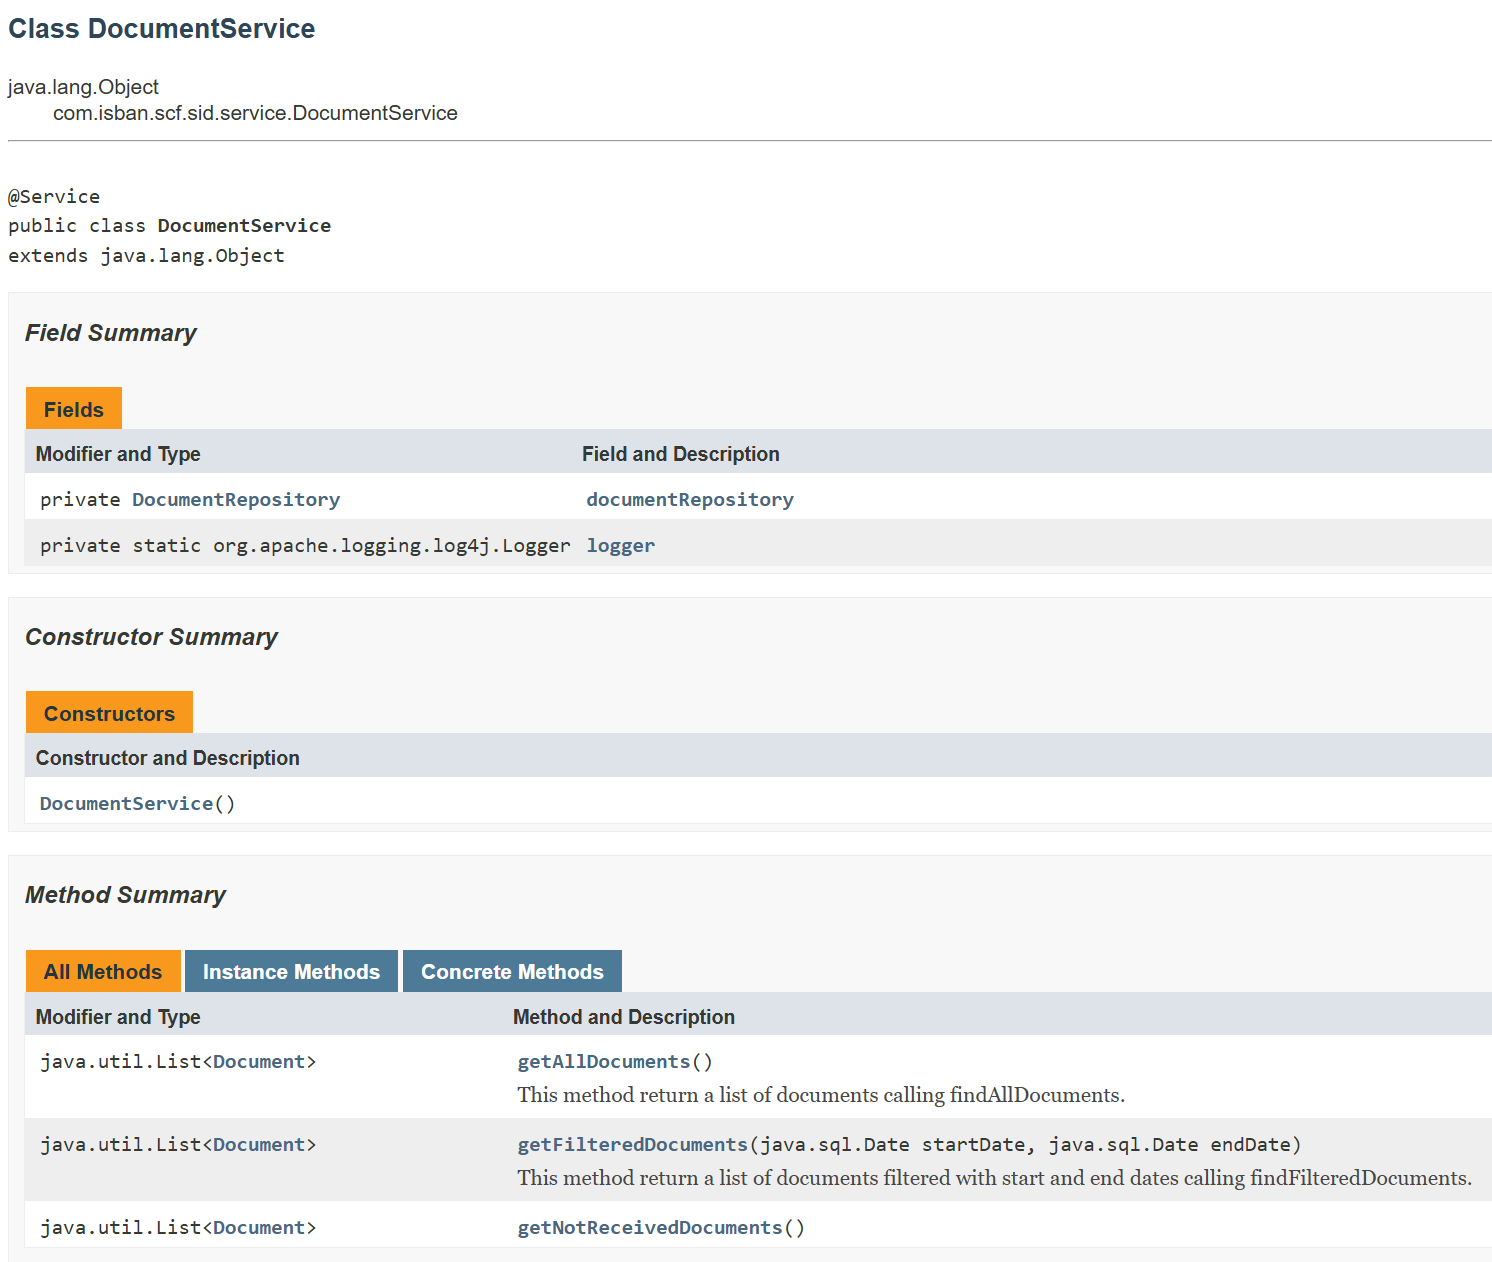
\includegraphics[width=0.5\linewidth]{javadoc-SIDManager.png}
%     \caption{Interfaz web de Javadoc para la clase \emph{DocumentService}}
%     \label{fig:javadoc-document-service}
% \end{figure}


% La implementación de Javadoc en la aplicación no solo mejora la comprensión del código para los desarrolladores, sino que también facilita su uso y mantenimiento. Esta práctica sigue los estándares de la industria y garantiza que cualquier persona que desee utilizar o modificar la aplicación pueda hacerlo de manera eficiente y con un mínimo de esfuerzo.




%
\chapter{Pruebas, validación y resultados}\label{resultados}
Las pruebas y la validación son etapas críticas en el desarrollo de cualquier sistema de software, ya que permiten garantizar que la aplicación cumple con los requisitos funcionales y no funcionales, además de asegurar su correcto funcionamiento en diferentes escenarios. A continuación, se describen las estrategias y metodologías utilizadas para validar el correcto funcionamiento de SIDManager, así como los resultados obtenidos durante este proceso.

\section{Estrategia de pruebas}
Para garantizar la calidad del software, se ha seguido una estrategia de pruebas que combina técnicas de prueba manual y automatizada. Esta estrategia se ha dividido en tres niveles principales:

\begin{itemize}    
    \item \textbf{Pruebas de integración}: Se han llevado a cabo pruebas para validar la interacción entre los diferentes componentes del sistema, como la conexión entre el backend y la base de datos, o la integración entre los servicios y los controladores. Estas pruebas han sido esenciales para detectar posibles errores en la comunicación entre módulos.
    
    \item \textbf{Pruebas de sistema}: Se han realizado pruebas end-to-end para validar el flujo completo de la aplicación, desde la interacción del usuario con la interfaz hasta la persistencia de datos en la base de datos. Estas pruebas han incluido escenarios como el registro de usuarios, la autenticación, la gestión de documentos y la recuperación de contraseñas.
\end{itemize}

\section{Validación de requisitos}
Durante las pruebas, se ha validado que la aplicación cumple con todos los requisitos, incluyendo:

\begin{itemize}
    \item \textbf{Funcionalidades principales}: Registro y autenticación de usuarios, gestión de documentos, filtrado por fechas y verificación del estado de los documentos.
    \item \textbf{Seguridad}: Validación del cifrado de contraseñas y manejo seguro de sesiones.
    \item \textbf{Rendimiento}: Evaluación del tiempo de respuesta de la aplicación bajo diferentes cargas de trabajo, garantizando un rendimiento óptimo incluso con grandes volúmenes de datos.
\end{itemize}


Los resultados obtenidos en el desarrollo de SIDManager demuestran que la aplicación cumple con los objetivos planteados inicialmente, ofreciendo una solución robusta, segura y escalable para la gestión y monitorización de documentos en entornos empresariales. A continuación, se presentan los resultados más relevantes del proyecto, tanto a nivel técnico como funcional.

\section{Resultados técnicos}
\begin{itemize}
    \item \textbf{Arquitectura modular}: La aplicación se ha desarrollado siguiendo una arquitectura basada en capas (vista, controlador, servicio, repositorio), lo que ha facilitado su mantenimiento y escalabilidad.
    \item \textbf{Seguridad implementada}: Se ha logrado un alto nivel de seguridad gracias al uso de Spring Security, el cifrado de contraseñas con BCrypt y la protección contra ataques comunes.
    \item \textbf{Integración de tecnologías modernas}: El uso de Spring Boot, Thymeleaf y JPA ha permitido desarrollar una aplicación eficiente y fácil de mantener.
    \item \textbf{Documentación completa}: El código ha sido documentado utilizando Javadoc, lo que facilita su comprensión y mantenimiento por parte de otros desarrolladores.
\end{itemize}

\section{Resultados funcionales}
\begin{itemize}
    \item \textbf{Gestión de documentos}: La aplicación permite filtrar y visualizar documentos de manera eficiente, verificando su correcto almacenamiento en la base de datos como se puede ver en las figuras \ref{fig:documentsView} y \ref{fig:documentsView_2}.
    \item \textbf{Autenticación y registro}: Los usuarios pueden registrarse, confirmar sus cuentas mediante correo electrónico y autenticarse de manera segura. Para ver la apariencia de la parte del registro consultar la figura \ref{fig:sign_up_view}.
    \item \textbf{Recuperación de contraseñas}: Se ha implementado un sistema seguro para la recuperación de contraseñas, utilizando códigos de confirmación únicos.
    \item \textbf{Interfaz intuitiva}: La interfaz de usuario, desarrollada con Thymeleaf y Bootstrap, es clara y fácil de usar, lo que mejora la experiencia del usuario.
\end{itemize}


\begin{figure}
    \centering
    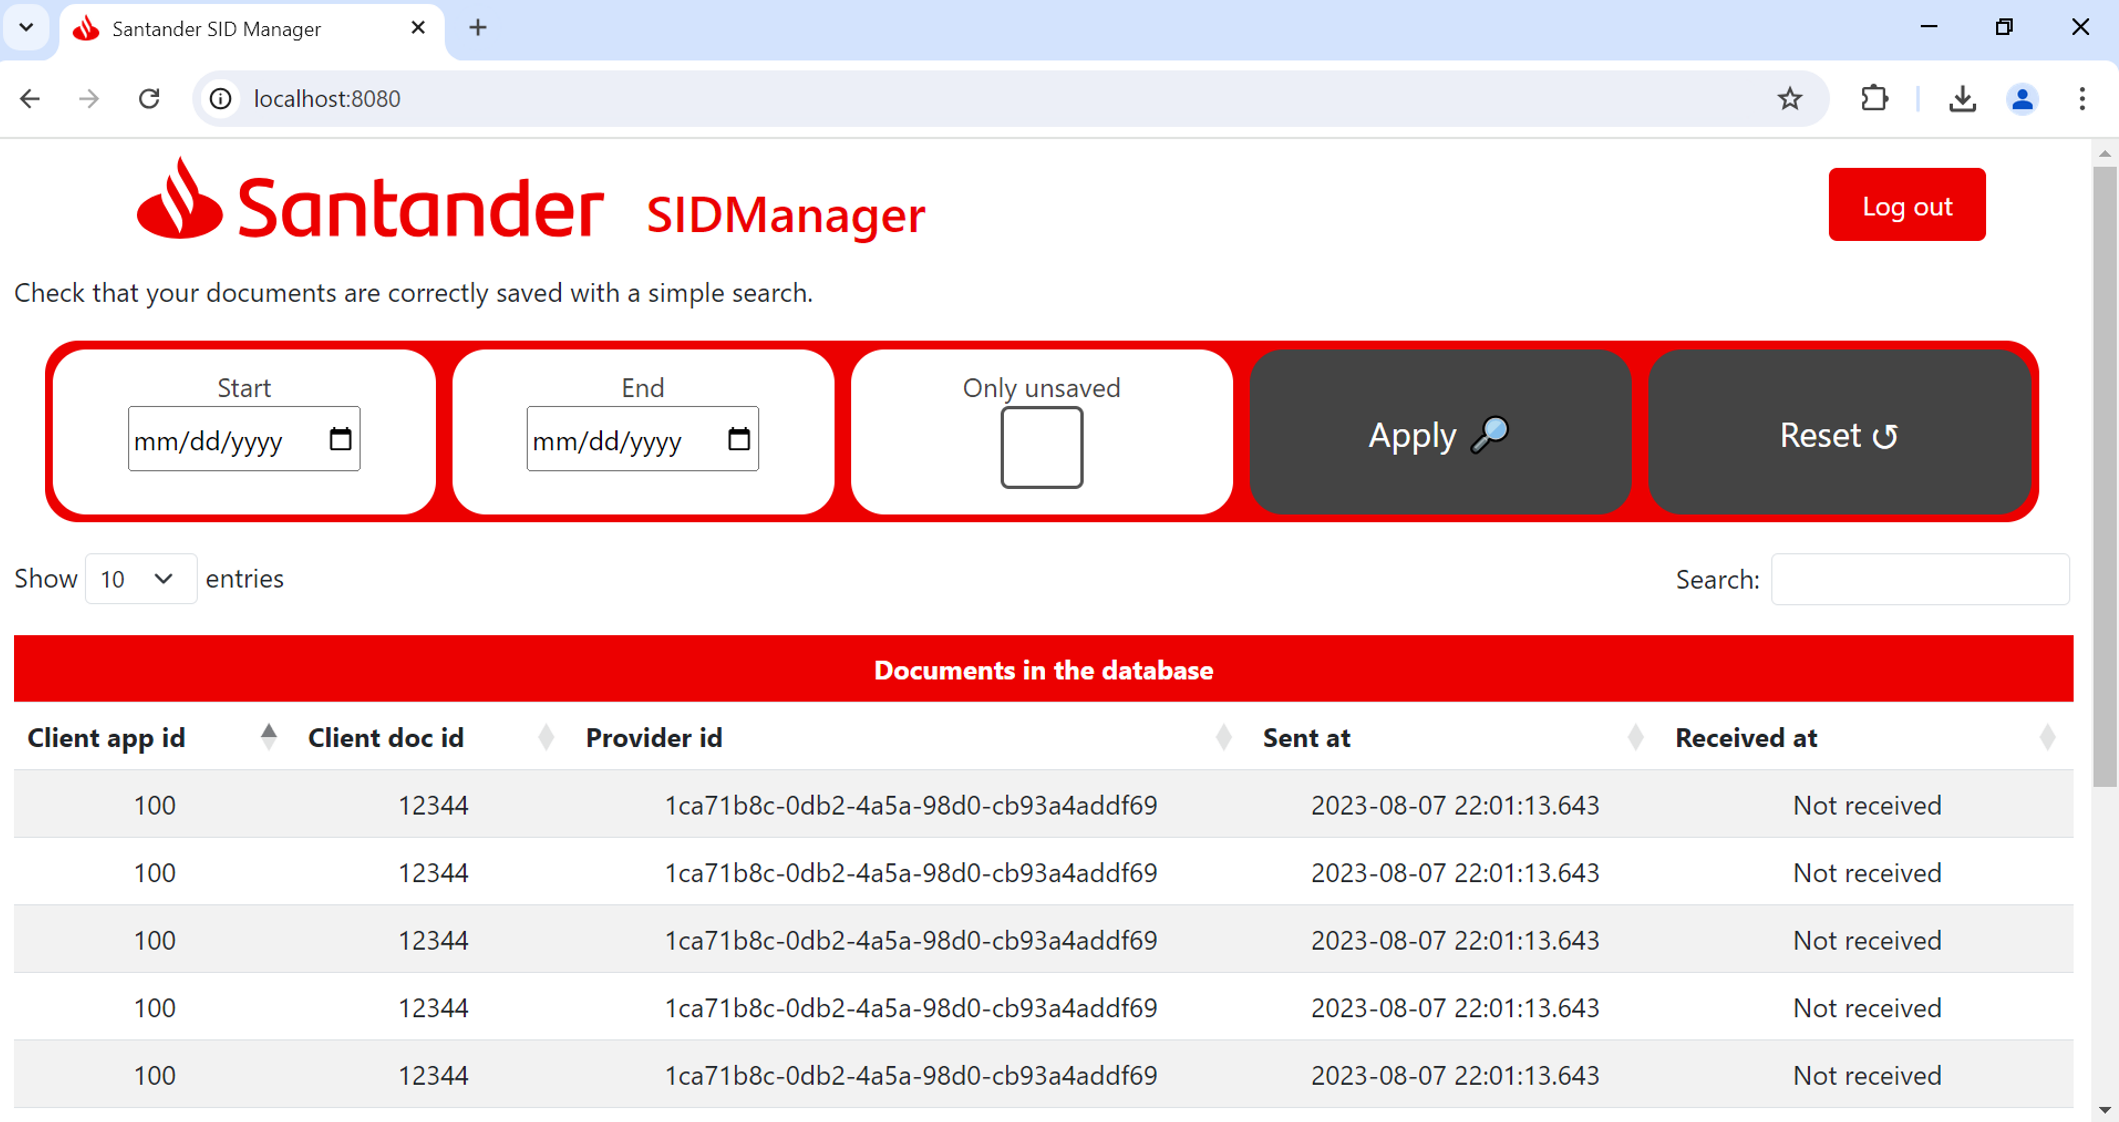
\includegraphics[width=0.75\linewidth]{imagenes/view/documentsView.png}
    \caption{Apariencia de la página principal de la aplicación SDIManager}
    \label{fig:documentsView}
\end{figure}

\begin{figure}
    \centering
    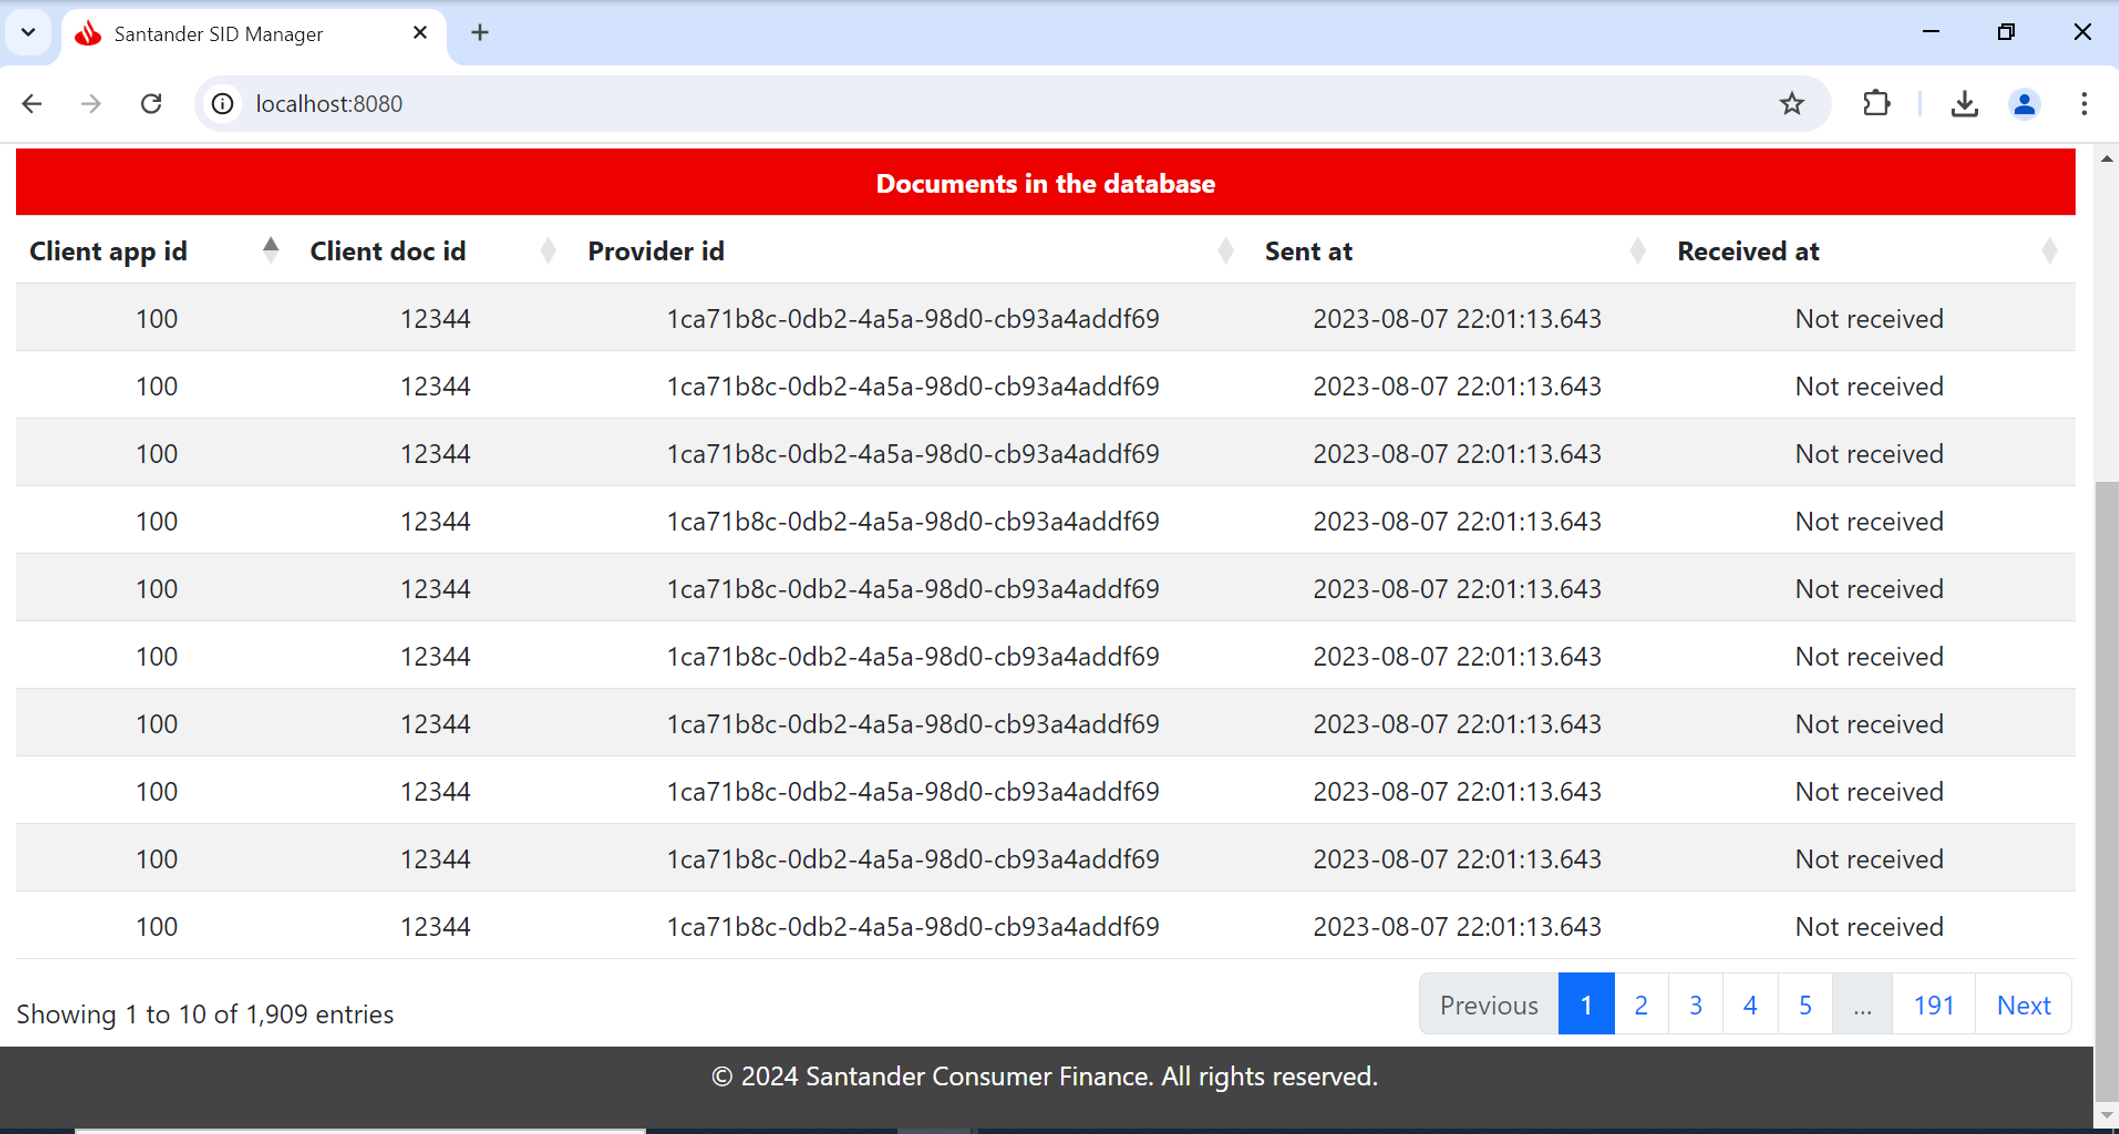
\includegraphics[width=0.75\linewidth]{imagenes/view/documentsView_2.png}
    \caption{Apariencia de la parte baja de página principal de la aplicación SDIManager}
    \label{fig:documentsView_2}
\end{figure}

\begin{figure}
    \centering
    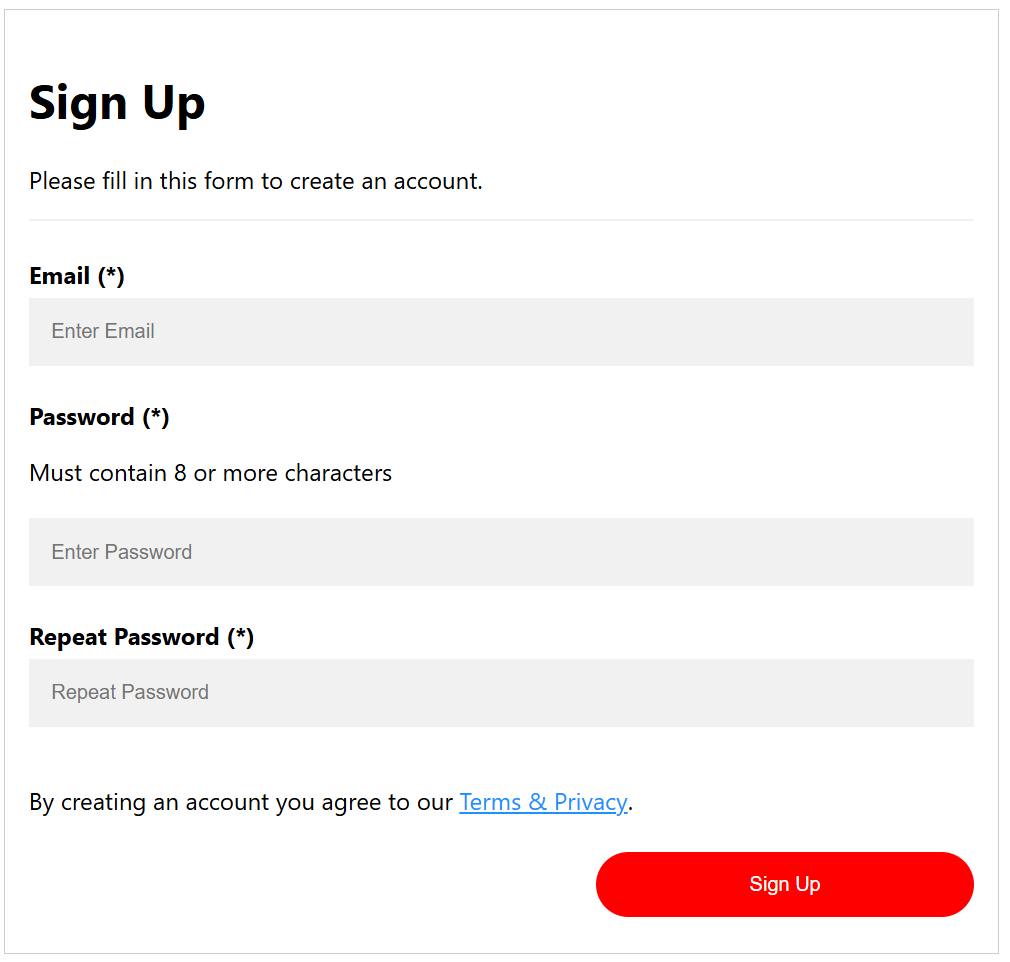
\includegraphics[width=0.75\linewidth]{imagenes/view/sign_up_view.png}
    \caption{Apariencia del registro de usuarios de la aplicación SDIManager}
    \label{fig:sign_up_view}
\end{figure}

Para más información de los resultados y las interfaces finales, se puede visualizar el video sobre la aplicación SIDManager en el siguiente enlace \url{https://youtu.be/DZQm53UCwSE}.
%
\chapter{Conclusiones y trabajos futuros}

Este capítulo sirve como cierre del proyecto y está dividido en dos secciones principales. En la Sección \ref{sec:conclusiones} se presenta un análisis que compara los objetivos alcanzados y aquellos que pueden mejorarse. En la Sección \ref{futuro} se proponen posibles mejoras y líneas de trabajo futuro, tanto en términos de investigación como de desarrollo adicional de la aplicación, además de una reflexión personal sobre el proceso de desarrollo.

\section{Conclusiones}
\label{sec:conclusiones}

Se ha cumplido con el objetivo principal de este TFG, desarrollando una aplicación funcional que resuelve de manera efectiva los problemas identificados en la gestión documental. A través de un proceso riguroso de análisis, diseño e implementación, se han alcanzado todos los objetivos planteados inicialmente con precisión, obteniendo así las siguientes conclusiones:

\begin{itemize}
    \item Planificación y organización: Hacer las cosas bien desde el principio ahorra tiempo y esfuerzo a largo plazo. Por ejemplo, la implementación de logs propios y el uso de archivos externos para mensajes de la aplicación han demostrado ser decisiones acertadas que facilitaron el mantenimiento y la depuración del código.
    
    \item Subestimación de tecnologías: Durante el desarrollo, se observó que algunas tecnologías o tareas aparentemente simples pueden resultar más complejas de lo esperado. Esto subraya la importancia de investigar y planificar adecuadamente antes de implementar soluciones.
    
    \item Documentación y buenas prácticas: Nombrar variables y clases de manera significativa y seguir estándares de codificación ha sido fundamental para mantener un código legible y fácil de mantener, especialmente en un proyecto con más de 60 archivos editados.
    
    \item Importancia de la modularidad: Separar los mensajes de la aplicación en archivos externos desde el principio ha demostrado ser una práctica muy útil, ya que evita la necesidad de modificar el código fuente cada vez que se requiere un cambio en los textos.

    \item Uso de tecnologías modernas: La elección de tecnologías como  Thymeleaf, en lugar de REST para el backend ha permitido aprovechar al máximo el potencial de SpringBoot. Sin embargo no ha permitido desacoplar el frontend del backend en su totalidad, lo que podría probocar problemas en  la escalabilidad y la integración con frameworks modernos como React o Angular.
\end{itemize}

En resumen, este proyecto ha sido una oportunidad para aplicar conocimientos previos, aprender nuevas herramientas y adoptar buenas prácticas de desarrollo. Aunque se han alcanzado los objetivos principales, siempre hay margen para mejorar y optimizar el trabajo realizado.

\section{Líneas de trabajo futuras}
\label{futuro}

A lo largo del desarrollo del proyecto, surgieron varias ideas y mejoras que, debido a limitaciones de tiempo y alcance, no pudieron implementarse. A continuación, se proponen algunas líneas de trabajo futuro para continuar mejorando la aplicación:

\begin{itemize}
    \item Implementación de un framework moderno para el frontend: Utilizar tecnologías como Vite, Next.js o un framework similar para el desarrollo del frontend, aprovechando el controlador REST ya implementado. Esto mejoraría la experiencia del usuario y facilitaría la creación de interfaces más dinámicas y responsivas.
    
    \item Paginación en la carga de documentos: Implementar un sistema de paginación para la carga de documentos, lo que mejoraría el rendimiento de la aplicación al manejar grandes volúmenes de datos.
    
    \item Buscador avanzado: Implementar un sistema de búsqueda avanzada que permita a los usuarios introducir identificadores específicos (como client\_app\_id o client\_doc\_id) para filtrar y localizar documentos de manera rápida y precisa. Esta funcionalidad mejoraría la usabilidad de la aplicación al permitir búsquedas más eficientes y reducir el tiempo necesario para encontrar información específica.
    
    \item Sistema de descarga de datos: Implementar un sistema integrado en la aplicación para facilitar la descarga de conjuntos de datos de la tabla con los documentos filtrados.
\end{itemize}

Estas propuestas representan oportunidades para seguir avanzando en el desarrollo de la aplicación y explorar nuevas áreas de investigación. La implementación de estas mejoras no solo mejoraría la funcionalidad y usabilidad de la aplicación, sino que también abriría nuevas posibilidades para su uso en entornos académicos y profesionales.



\chapter*{}
Personalmente, este proyecto ha sido una oportunidad para profundizar en tecnologías y conceptos que no formaban parte de mi conocimiento previo. Desde el aprendizaje de nuevas herramientas como Spring Boot y Maven hasta la adopción de buenas prácticas como la documentación con Javadoc y el uso de estándares de Java, he adquirido habilidades que serán valiosas en futuros proyectos. Además, la experiencia de trabajar en un proyecto de esta envergadura ha reforzado mi capacidad para planificar, organizar y resolver problemas de manera eficiente.

En conclusión, este proyecto no solo ha cumplido con sus objetivos iniciales, sino que también ha sentado las bases para futuras mejoras y desarrollos. Espero que el trabajo realizado contribuya al avance de aplicaciones similares y sirva como referencia para otros desarrolladores e investigadores.

%%\nocite{*} %incluye TODOS los documentos de la base de datos bibliográfica sean o no citados en el texto
\newpage
\printbibliography

%\bibliography{bibliografia/bibliografia}
%\addcontentsline{toc}{chapter}{Bibliografía} %sustituir bibliografía con el nombre del fichero bibtex con la bibliografía
%


\appendix
\chapter{Anexo I. Esquema de base de datos}


\begin{figure}
    \centering
    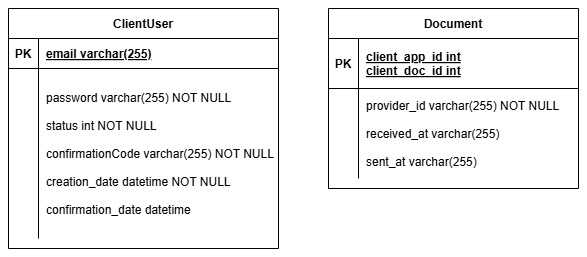
\includegraphics[width=0.5\linewidth]{imagenes//scheme/SIDManager_BD.jpg}
    \caption{Esquema de  la base de datos}
    \label{fig:BD-scheme}
\end{figure}

\chapter{Anexo II. Código de la aplicación SIDManager}

\begin{lstlisting}[
    language=xml,
    label=code:kachiquel_xml,
    caption={Kaqchikel XML generado por el LLM a partir de la imagen de la página original}
]
<?xml version="1.0" encoding="UTF-8"?>
<document>
    <page number="203">
        <heading>... / .. / .... Oración compleja</heading>
        <line>La oración compleja se forma con más de una cláusula, una de ellas es la principal y</line>
        <line>otra la subordinada. La idea que expresan las cláusulas subordinadas siempre dependen</line>
        <line>de la cláusula principal, su posición es siempre después de ésta. Una cláusula subordinada</line>
        <line>se introduce por medio de subordinadores, aunque hay excepciones. Son oraciones</line>
        <line>complejas si dentro de la cláusula principal se encuentran las siguientes cláusulas</line>
        <line>subordinadas:</line>
       
        <line>Cláusula relativa</line>
        <line>Cláusula adjunta o adverbial</line>
        <line>Cláusula de complemento</line>


        <heading>... / .. / .... / . Clausula relativa</heading>
        <line>La clausula relativa modifica a sustantivos, describe alguna caracteristica, por eso</line>
        <line>funciona como adjetivo. La clausula relativa se introduce por los subordinadores: ri,</line>
        <line>re, la, achoq rik'in y achoq chi re o simplemente subordinador. Estas particulas se</line>
        <line>conocen con los nombres de pronombre relativo o relativizador. Si modifica al sujeto u</line>
        <line>objeto, se introduce con las particulas: ri, re, la. Si modifica al instrumento o compania,</line>
        <line>la clausula relativa se introducen con la frase achoq rik'in; y si la clausula no se</line>
        <line>introduce por subordinador, la clausula relativa se escribe entre comas. Ejemplos:</line>


        <line>Modificando al sujeto:</line>
        <interlinear_gloss>
            <parallel_phrase>
                <original>Ri ix\"{o}q, ri xkos, xb'eruloq'o' xkoya'.</original>
                <translation>La mujer que se cansó fue a comprar tomate</translation>
            </parallel_phrase>
            <morpheme_analysis>
                <unit>
                    <form>Ri</form>
                    <gloss>DET</gloss>
                </unit>
                <unit>
                    <form>ix\"{o}q,</form>
                    <gloss>mujer</gloss>
                </unit>
                <unit>
                    <form>ri</form>
                    <gloss>CR</gloss>
                </unit>
                <unit>
                    <form>x-</form>
                    <gloss>COM-</gloss>
                </unit>
                <unit>
                    <form>{\O}-</form>
                    <gloss>B3s-</gloss>
                </unit>
                <unit>
                    <form>kos,</form>
                    <gloss>cansar</gloss>
                </unit>
                <unit>
                    <form>x-</form>
                    <gloss>COM-</gloss>
                </unit>
                <unit>
                    <form>{\O}-</form>
                    <gloss>B3s-</gloss>
                </unit>
                <unit>
                    <form>b'e-</form>
                    <gloss>MOV-</gloss>
                </unit>
                <unit>
                    <form>ru-</form>
                    <gloss>A3s-</gloss>
                </unit>
                <unit>
                    <form>loq'-</form>
                    <gloss>comprar-</gloss>
                </unit>
                <unit>
                    <form>o'</form>
                    <gloss>SC</gloss>
                </unit>
                <unit>
                    <form>xkoya'.</form>
                    <gloss>tomate</gloss>
                </unit>
            </morpheme_analysis>
            <syntactic_analysis>
                <unit>
                    <form>ri xkos</form>
                    <gloss>CR</gloss>
                </unit>
            </syntactic_analysis>
        </interlinear_gloss>


        <interlinear_gloss>
            <parallel_phrase>
                <original>Re ak'wal, re xtzaq, xoq'.</original>
                <translation>Este niño que se cayó, lloró.</translation>
            </parallel_phrase>
            <morpheme_analysis>
                <unit>
                    <form>Re</form>
                    <gloss>DET</gloss>
                </unit>
                <unit>
                    <form>ak'wal,</form>
                    <gloss>niño,</gloss>
                </unit>
                <unit>
                    <form>re</form>
                    <gloss>CR</gloss>
                </unit>
                <unit>
                    <form>x-</form>
                    <gloss>COM-</gloss>
                </unit>
                <unit>
                    <form>{\O}-</form>
                    <gloss>B3s-</gloss>
                </unit>
                <unit>
                    <form>tzaq,</form>
                    <gloss>caer</gloss>
                </unit>
                <unit>
                    <form>xoq'.</form>
                    <gloss>llorar</gloss>
                </unit>
            </morpheme_analysis>
            <syntactic_analysis>
                <unit>
                    <form>re xtzaq</form>
                    <gloss>CR</gloss>
                </unit>
            </syntactic_analysis>
        </interlinear_gloss>


        <interlinear_gloss>
            <parallel_phrase>
                <original>La k'aj\"{o}l, la xloq'o ri wexaj, xb'e.</original>
                <translation>Ese muchacho que compr\'o el pantal\'on, se fue.</translation>
            </parallel_phrase>
            <syntactic_analysis>
                <unit>
                    <form>la xloq'o ri wexaj</form>
                    <gloss>CR</gloss>
                </unit>
            </syntactic_analysis>
        </interlinear_gloss>
    </page>
</document>

}
\end{lstlisting}

\begin{lstlisting}[
    language=Java, 
    label=code:not-received-controller, 
    caption={Función getNotReceivedDocuments del controlador}
]
@GetMapping ("/not-received")
public String getNotReceivedDocuments(Model model){
    logger.debug(" ----- Entering getNotReceivedDocuments ----- " );
    model.addAttribute("documents" , documentService.getNotReceivedDocuments());
    model.addAttribute ("isShowingUnsaveds", "Yes");
    logger.debug(" ----- Exiting getNotReceivedDocuments ----- ");
    return "documentsView";
}
\end{lstlisting}



\begin{lstlisting}[
    language=Java,
    label={code:not-received-service},
    caption={Función getNotReceivedDocuments del servicio}
]
public List<Document> getNotReceivedDocuments() {
    logger.debug(" Entering getNotReceivedDocuments ");
    return documentRepository.findByReceivedAtIsNull();
}
\end{lstlisting}



\begin{lstlisting}[
    language=Java, 
    label=code:list-docs,
    caption={Función listDocuments del controlador}
]
@GetMapping("/list")
public String listDocuments(
        @RequestParam(value = "min-date",  required = false) String startDate,
        @RequestParam(value = "max-date", required = false) String endDate,
        Model model) throws Exception {
    logger.debug(" ----- Entering listDocuments ----- ");
    
    DateRange dateRange = documentService.checkDates(startDate, endDate, model);
    
    model.addAttribute("documents", 
            documentService.getFilteredDocuments(
                    dateRange.getStartDate(),
                    dateRange.getEndDate()
                    ));    	
    model.addAttribute("startDate", dateRange.getStartDate());
    model.addAttribute("endDate", dateRange.getEndDate());
    model.addAttribute("isShowingUnsaveds", "No");
    
    logger.debug(" ----- Exiting listDocuments ----- ");
    logger.debug(" ____________________________________ ");
        
    return "documentsView";
}
\end{lstlisting}



\begin{lstlisting}[
    language=Java, 
    label=code:list-docs-service,
    caption={Función getFilteredDocuments del servicio}
]
public List<Document> getFilteredDocuments(Date startDate, Date endDate) {
    logger.debug(" Entering getFilteredDocuments ");
    return documentRepository.findFilteredDocuments(startDate, endDate);
}
\end{lstlisting}



\begin{lstlisting}[
    language=Java,
    label=code:list-docs-repositoty,
    caption={Función findFilteredDocuments del repositorio}
]
@Query(value = "SELECT CLIENT_APP_ID, CLIENT_DOC_ID, PROVIDER_ID, SENT_AT, RECEIVED_AT"
            + " FROM documents WHERE SENT_AT > :startDate AND SENT_AT < :endDate", nativeQuery = true)
List<Document> findFilteredDocuments(@Param("startDate") Date startDate, @Param("endDate") Date endDate); 
\end{lstlisting}



\begin{lstlisting}[
    language=Java, 
    label={code:checkDates},
    caption={Función checkDates del servicio}
]
public DateRange checkDates(String stringStartDate, String stringEndDate, Model model) {
    final int daysRange = 10;  
    DateRange dateRange;
    boolean isCorrectRange = true;
    
    try {
        if (DateUtils.checkDate(stringStartDate) && DateUtils.checkDate(stringEndDate)) {
            Date startDate = DateUtils.stringToUtilsDate(stringStartDate);
            Date endDate = DateUtils.stringToUtilsDate(stringEndDate);
            
            int daysBetween = DateUtils.daysBetween(startDate, endDate);
            
            if(daysBetween != -1 && daysBetween <= daysRange) {
                dateRange = new DateRange(startDate, endDate);
                logger.info(" Returning FILTERED documents ");
            } else {
                dateRange = new DateRange(-daysRange);
                
                logger.warn(" Exceded maximum day range ( " +
                            daysBetween + 
                            " ) with: " + 
                            daysRange);
                logger.warn(" Returning last 10 days ");
                
                isCorrectRange = false;
            }
        } else if (DateUtils.checkDate(stringEndDate)) {
            dateRange = new DateRange(DateUtils.stringToUtilsDate(stringEndDate), -daysRange);
            isCorrectRange = false;
        } else if (DateUtils.checkDate(stringStartDate)) {
            dateRange = new DateRange(DateUtils.stringToUtilsDate(stringStartDate), daysRange);
            isCorrectRange = false;
        } else {
            dateRange = new DateRange(-daysRange);
        }
    } catch (ParseException e) {
        logger.error(" ERROR in getFilteredDocuments: " + e);
        dateRange = new DateRange(-daysRange);			
    }
    
    if (!isCorrectRange) {
        model.addAttribute("responseMessage", ResponseEnum.LIST_WARNING_1.getMessageKey());
        model.addAttribute("isAWarningMessage", true);
    }
    
    return dateRange;
}
\end{lstlisting}



\begin{lstlisting}[
    language=Java, 
    label=code:getCreateClientUserView,
    caption={Función getCreateClientUserView del controlador}
]
@GetMapping("/user/create")
public String getCreateClientUserView() {
    logger.debug("Entering GET: /user/create");
    
    return "createClientUserView"; 
}
\end{lstlisting}



\begin{lstlisting}[
    language=Java,
    label=code:createClientUser-controller,
    caption={Función createClientUser del controlador}
]
@PostMapping("/user/create")
public String createClientUser(Model model, 
                                @ModelAttribute ClientUser clientUser,
                                @RequestParam("psw-repeat") String passwordRepeat
                                ) throws Exception {
    
    logger.debug(" - Entering clientUserService.createClientUser(), from POST: /user/create");
    
    ResponseEnum responseMessage = clientUserService.createClientUser(clientUser, passwordRepeat);

    model.addAttribute("responseMessage", responseMessage.getMessageKey());
    addColorToResponse(model, responseMessage);
    
    return "createClientUserView";  
}
\end{lstlisting}



\begin{lstlisting}[
    language=Java,
    label=code:saveClientUser-controller,
    caption={Función saveClientUser del controlador}
]
@Transactional
public ClientUser saveClientUser(ClientUser clientUser) throws Exception {
    try {
        if (clientUser.getPassword() != null) {
            logger.debug(" -- Entering encryptMessage()");
            clientUser.setPassword(encryptFacade(clientUser.getPassword()));
            
            logger.debug(" -- Entering randomAlphanumeric()");
            clientUser.setConfirmationCode(RandomStringUtils.randomAlphanumeric(30));
            
            clientUser.setStatus(0);
            clientUser.setCreationDate(new Date()); 
            clientUserRepository.save(clientUser);
        } else {
             throw new IllegalArgumentException("Password cannot be null");
        }
    } catch (Exception e) {
        logger.error(" ERROR: Possible error in encryption, confirmation code generation "
                + " or saveClientUser:" + e);
        throw e;
    }
    
    return clientUser;
}
\end{lstlisting}



\begin{lstlisting}[
    language=Java,
    label=code:getConfirmation-controller,
    caption={Función getConfirmation del controlador}
]
@GetMapping("/user/confirm")
public String getConfirmation(Model model, 
                              @RequestParam("email") String email,
                              @RequestParam("confirmationCode") String confirmationCode) {
    
    logger.debug(" - Entering clientUserService.confirmUser(), from GET: /user/confirm");
    ResponseEnum responseMessage = clientUserService.confirmUser(email, confirmationCode);
    logger.debug(" - Exiting clientUserService.confirmUser()");
    
    model.addAttribute("responseMessage", responseMessage.getMessageKey());
    addColorToResponse(model, responseMessage);
    
    return "confirmationUser"; 
}    
\end{lstlisting}


\begin{lstlisting}[
    language=Java,
    label=code:confirmUser-service,
    caption={Función confirmUser del servicio}
]
@Transactional
public ResponseEnum confirmUser(String email,
                                String confirmationCode
                                ) {
    ResponseEnum responseMessage;
    ClientUser clientUser = clientUserRepository.findByEmailAndConfirmationCodeAndStatus(email, confirmationCode, 0);	
    
    if (clientUser != null) {
        responseMessage = ResponseEnum.CONFIRM_SUCCESS;
        clientUser.setStatus(1);
        clientUser.setConfirmationDate(new Date()); 
        clientUserRepository.save(clientUser);
    } else {
        logger.debug(" User not found, not correct or already confirmed. ");
        responseMessage = ResponseEnum.CONFIRM_WARNING;
    }
    
    return responseMessage;
}
\end{lstlisting}


\begin{lstlisting}[
    language=Java,
    label=code:getLoginView-controller,
    caption={Función getLoginView del controlador}
]
@GetMapping("/user/login")
public String getLoginView(Model model,
                           HttpServletRequest request
                           ) throws Exception {
    String serverUrl = SharedProperties.get("serverUrl");
    String requestUpdatePasswordUrl =  serverUrl + "user/requestUpdatePassword";
    String createClientUserUrl = serverUrl + "user/create";
    String errorMessage = (String) request.getSession().getAttribute("error");
    
    model.addAttribute("requestUpdatePasswordUrl", requestUpdatePasswordUrl);
    model.addAttribute("createClientUserUrl", createClientUserUrl);
    
    if (errorMessage != null) {
        ResponseEnum responseMessage = ResponseEnum.LOGIN_WARNING_1;
        model.addAttribute("responseMessage", responseMessage.getMessageKey());
        addColorToResponse(model, responseMessage);
        
        // Elimina el mensaje de error de la sesión
        request.getSession().removeAttribute("error");
    }
    
    return "loginView";
}
\end{lstlisting}



\begin{lstlisting}[
    language=Java,
    label=code:getRequestUpdatePasswordView-controller,
    caption={Función getRequestUpdatePasswordView del controlador}
]
@GetMapping("/user/requestUpdatePassword")
public String getRequestUpdatePasswordView() {
    return "requestUpdatePasswordView";
}
\end{lstlisting}



\begin{lstlisting}[
    language=Java,
    label=code:requestUpdatePassword-controller,
    caption={Función requestUpdatePassword del controlador}
]
@PostMapping("user/requestUpdatePassword")
public String requestUpdatePassword(Model model,
        @RequestParam("email") String email
        ) throws Exception  {
    
    ResponseEnum responseMessage = clientUserService.sendUpdatePasswordUrl(email);
    
    model.addAttribute("responseMessage", responseMessage.getMessageKey());
    addColorToResponse(model, responseMessage);
    
    return "requestUpdatePasswordView";
}
\end{lstlisting}




\begin{lstlisting}[
    language=Java,
    label=code:sendUpdatePasswordUrl-service,
    caption={Función sendUpdatePasswordUrl del servicio}
]
public ResponseEnum sendUpdatePasswordUrl(String email) throws Exception {
    ResponseEnum responseMessage;
    ClientUser clientUser = clientUserRepository.findByEmail(email);
    
    if (clientUser != null && clientUser.getStatus() == 1) {
        String path = "user/updatePassword?email=";
        String urlUpdatePassword = this.getConfirmationUrl(clientUser, path);
        
        logger.debug(" - Entering sendMail");
        String subject = " Change the password of your SIDManager user. ";
        String body = " Click on the next URL if you want to change your password: ";
        Mail.sendMail(clientUser.getEmail(), urlUpdatePassword, subject, body);
        logger.debug(" - Exiting sendMail");
        
        responseMessage = ResponseEnum.UPDATE_PSW_SUCCESS_1;
    } else {
        responseMessage = ResponseEnum.UPDATE_PSW_WARNING_1;
        logger.info(" The user does not exist or is not confirmed. ");
    }

    return responseMessage;
}
\end{lstlisting}



\begin{lstlisting}[
    language=Java,
    label=code:getConfirmationUrl-service,
    caption={Función getConfirmationUrl del servicio}
]
private String getConfirmationUrl(ClientUser clientUser,
      String path
      ) throws Exception {
    StringBuilder confirmationUrl = new StringBuilder();
    String serverUrl = SharedProperties.get("serverUrl");
    
    confirmationUrl.append(serverUrl);
    confirmationUrl.append(path);
    confirmationUrl.append(clientUser.getEmail());
    confirmationUrl.append("&confirmationCode=");
    confirmationUrl.append(clientUser.getConfirmationCode());
    
    return confirmationUrl.toString();
}
\end{lstlisting}



\begin{lstlisting}[
    language=Java,
    label=code:getUpdatePasswordView-controller,
    caption={Función getUpdatePasswordView del controlador}
]
@GetMapping("/user/updatePassword")
public String getUpdatePasswordView(Model model, 
        HttpSession session,
        @RequestParam("email") String email,
        @RequestParam("confirmationCode") String confirmationCode
        ) throws Exception {
    boolean shouldFormBeShown = false;
    ResponseEnum responseMessage = clientUserService.getUpdatePasswordView(email, confirmationCode);
    
    if (responseMessage.getStatus() == ResponseEnum.UPDATE_PSW_SUCCESS_2.getStatus()) {
        shouldFormBeShown = true;
    } else {
        model.addAttribute("responseMessage", responseMessage.getMessageKey());
        addColorToResponse(model, responseMessage);
    }
    
    model.addAttribute("shouldFormBeShown", shouldFormBeShown);
    
    //Save the email to send it later in the post
    session.setAttribute("email", email);
    
    return "updatePasswordView";
}
\end{lstlisting}



\begin{lstlisting}[
    language=Java,
    label=code:getUpdatePasswordView-service,
    caption={Función getUpdatePasswordView del servicio}
]
public ResponseEnum getUpdatePasswordView(String email,
                                          String confirmationCode
                                          ) {
    ResponseEnum responseMessage;
    ClientUser clientUser 
        = clientUserRepository.findByEmailAndConfirmationCodeAndStatus(
                email, confirmationCode, 1);	

    if (clientUser != null) {
        responseMessage = ResponseEnum.UPDATE_PSW_SUCCESS_2;
    } else {
        responseMessage = ResponseEnum.UPDATE_PSW_WARNING_2;
        logger.info(responseMessage.getMessageKey());
    }
    
    return responseMessage;
}
\end{lstlisting}




\begin{lstlisting}[
    language=Java,
    label=code:updatePassword-controller,
    caption={Función updatePassword del controlador}
]
@PostMapping("/user/updatePassword")
    public String updatePassword( Model model,
              HttpSession session,
              @ModelAttribute ClientUser clientUser,
              @RequestParam("psw-repeat") String passwordRepeat
              ) throws Exception {
        String loginUrl = SharedProperties.get("serverUrl") + "user/login";
        String email = (String) session.getAttribute("email");
        boolean shouldFormBeShown = true;
        ResponseEnum responseMessage = clientUserService.updatePassword(email, clientUser, passwordRepeat);
    	
        if (responseMessage.getStatus() == ResponseEnum.UPDATE_PSW_SUCCESS_3.getStatus()) {
            shouldFormBeShown = false;
            model.addAttribute("loginUrl", loginUrl);
        } 
    	
        model.addAttribute("responseMessage", responseMessage.getMessageKey());
        model.addAttribute("shouldFormBeShown", shouldFormBeShown);
        addColorToResponse(model, responseMessage);
        
        return "updatePasswordView";
    }
\end{lstlisting}



\begin{lstlisting}[
    language=Java,
    label=code:updatePassword-service,
    caption={Función updatePassword del servicio}
]
public ResponseEnum updatePassword(String email, 
           ClientUser clientUser, 
           String passwordRepeat
           ) throws Exception {
		ResponseEnum responseMessage;
		String password = clientUser.getPassword();
		
		 if (password != null && password.equals(passwordRepeat)) {
	        	// Check if the user exists in the database
		        ClientUser existingUser = this.getClientUser(email);
		        
		        if (existingUser != null) {
		        	existingUser.setPassword(encryptFacade(password));
		        	clientUserRepository.save(existingUser);
		            
		            responseMessage = ResponseEnum.UPDATE_PSW_SUCCESS_3;
		        } else {
		        	responseMessage = ResponseEnum.UPDATE_PSW_WARNING_4;
		        }
	        } else {
	        	responseMessage = ResponseEnum.UPDATE_PSW_WARNING_3;
	        }      
		
		return responseMessage;
	}
\end{lstlisting}



\begin{lstlisting}[
    language=Java,
    label=code:DocumentModel,
    caption={Clase DocumentModel}
]
package com.isban.scf.sid.model;

import javax.persistence.Column;
import javax.persistence.Entity;
import javax.persistence.Id;
import javax.persistence.Table;

@Entity
@Table(name = "documents") // Nombre de la tabla en la base de datos
public class Document {
@Id
@Column(name = "CLIENT_DOC_ID")
private Long clientDocId; 

@Column(name = "CLIENT_APP_ID")
private Long clientAppId; 

@Column(name = "PROVIDER_ID")
private String providerId; 

@Column(name = "SENT_AT")
private String sentAt;

@Column(name = "RECEIVED_AT")
private String receivedAt;

// Getters y setters
public Long getClientDocId() {
    return clientDocId;
}

public void setClientDocId(Long clientDocId) {
    this.clientDocId = clientDocId;
}

public Long getClientAppId() {
    return clientAppId;
}

public void setClientAppId(Long clientAppId) {
    this.clientAppId = clientAppId;
}

public String getProviderId() {
    return providerId;
}

public void setProviderId(String providerId) {
    this.providerId = providerId;
}

public String getSentAt() {
    return sentAt;
}

public void setSentAt(String sentAt) {
    this.sentAt = sentAt;
}

public String getReceivedAt() {
    return receivedAt;
}

public void setReceivedAt(String receivedAt) {
    this.receivedAt = receivedAt;
}

\end{lstlisting}




\begin{lstlisting}[
    language=Java,
    label=code:SecurityConfig,
    caption={Clase SecurityConfig}
]
@Configuration
@EnableWebSecurity
public class SecurityConfig {
	
    private final UserDetailsService userDetailsService;
	
    public SecurityConfig(UserDetailsService userDetailsService) {
        this.userDetailsService = userDetailsService;
    }
	
	@Bean
	public SecurityFilterChain securityFilterChain(HttpSecurity http) throws Exception {
	    http
	        .authorizeHttpRequests(authorizeRequests ->
	            authorizeRequests
	                .antMatchers("/user/login", 
                             "/user/create",
                             "/user/confirm", 
                             "/user/requestUpdatePassword",
                             "/user/updatePassword",
                             "/user/getAll",
                             "/user/deleteAll",
                             "/home",
                             "/css/**",
                             "/img/**",
                             "/js/**" 
                             ).permitAll() // Permitir acceso sin autenticación
	                .anyRequest().authenticated() // Cualquier otra ruta requiere autenticación
	        )
	        .formLogin(formLogin ->
	            formLogin
	                .loginPage("/user/login") // Página de login personalizada
	                .defaultSuccessUrl("/list", true) // Redirigir al home después del login exitoso
	                .permitAll()
	                .failureHandler(authenticationFailureHandler())
	        )
	        .logout(logout ->
	            logout
	                .logoutUrl("/logout")
	                .logoutSuccessUrl("/user/login?logout") // Redirigir a login después del logout
	                .invalidateHttpSession(true)
	                .deleteCookies("JSESSIONID")
	                .permitAll()
	        )
	        .exceptionHandling(exceptionHandling -> 
	            exceptionHandling.accessDeniedPage("/user/accessDenied")); // Manejo de accesos denegados

	    return http.build();
	}
	    
    protected void configure(AuthenticationManagerBuilder auth) throws Exception {
        auth.userDetailsService(userDetailsService).passwordEncoder(passwordEncoder());
    }
    
    @Bean
    public PasswordEncoder passwordEncoder() {
        return new BCryptPasswordEncoder();
    }
    
    @Bean
    public AuthenticationFailureHandler authenticationFailureHandler() {
        return new CustomAuthenticationFailureHandler();
    }    
    
}
\end{lstlisting}



\begin{lstlisting}[
    language=Java,
    label=code:CustomUserDetailsService,
    caption={Clase CustomUserDetailsService}
]

@Service
public class CustomUserDetailsService implements UserDetailsService {

	private final ClientUserRepository clientUserRepository;
	
    public CustomUserDetailsService(ClientUserRepository userRepository) {
        this.clientUserRepository = userRepository;
    }
    
    @Override
    public UserDetails loadUserByUsername(String username) throws UsernameNotFoundException {
        ClientUser user = clientUserRepository.findByEmail(username);
        
        if (user == null) {
            throw new UsernameNotFoundException("User not found");
        }
        
        CustomUserDetails customUserDetails = new CustomUserDetails(user);
        
        return customUserDetails;
    }
}
\end{lstlisting}



\begin{lstlisting}[
    language=Java,
    label=code:CustomUserDetailsService-modified,
    caption={Clase CustomUserDetailsService modificado}
]

@Service
public class CustomUserDetailsService implements UserDetailsService {

	private final ClientUserRepository clientUserRepository;
	
    public CustomUserDetailsService(ClientUserRepository userRepository) {
        this.clientUserRepository = userRepository;
    }
    
    @Override
    public UserDetails loadUserByUsername(String username) throws UsernameNotFoundException {
        ClientUser user = clientUserRepository.findByEmail(username);
        
        if (user == null) {
            throw new UsernameNotFoundException("User not found");
        }
        
        CustomUserDetails customUserDetails = new CustomUserDetails(user);
        
        return customUserDetails;
    }
}
\end{lstlisting}




\begin{lstlisting}[
    language=Java,
    label=code:CustomAuthenticationFailureHandler,
    caption={Clase CustomAuthenticationFailureHandler}
]
@Component
public class CustomAuthenticationFailureHandler implements AuthenticationFailureHandler {

    @Override
    public void onAuthenticationFailure(HttpServletRequest request, HttpServletResponse response, AuthenticationException exception) 
      throws IOException, ServletException {
        // Establece un mensaje de error en la sesión
        request.getSession().setAttribute("error", "Login error");
        
        // Redirige de nuevo a la página de login
        response.sendRedirect("/user/login");
    }
    
}
\end{lstlisting}


\begin{lstlisting}[
    language=Java,
    label=code:encryptMessage,
    caption={Función encryptMessage de Encryptor}
]
public static String encryptMessage(String message) throws Exception {
    if (message == null) {
        throw new IllegalArgumentException("Message to be encrypted cannot be null");
    } 
    byte[] key = SharedProperties.getEncryptKey().getBytes();
    
    Cipher cipher = Cipher.getInstance(ALGORITHM);
    SecretKeySpec secretKey = new SecretKeySpec(key, "AES");
    cipher.init(Cipher.ENCRYPT_MODE, secretKey);
    byte[] encryptedMessage = cipher.doFinal(message.getBytes());
    
    return Base64.getEncoder().encodeToString(encryptedMessage);
}
\end{lstlisting}



\begin{lstlisting}[
    language=Java,
    label=code:decryptMessage,
    caption={Función decryptMessage de Encryptor}
]
public static String decryptMessage(String encryptedMessage) throws Exception {
    byte[] key = SharedProperties.getEncryptKey().getBytes();
    
    byte[] messageBytes = Base64.getDecoder().decode(encryptedMessage);
    Cipher cipher = Cipher.getInstance(ALGORITHM);
    SecretKeySpec secretKey = new SecretKeySpec(key, "AES");
    cipher.init(Cipher.DECRYPT_MODE, secretKey);
    byte[] decryptedBytes = cipher.doFinal(messageBytes);
    
    return new String(decryptedBytes);
}
\end{lstlisting}




\begin{lstlisting}[
    language=Java,
    label=code:getDataSource,
    caption={La función getDataSource de DataSourceConfig}
]
@Bean
@Primary
public DataSource getDataSource() {
    logger.debug(" --- Creating driver for database connection --- ");
    
    DriverManagerDataSource dataSource = new DriverManagerDataSource();
    dataSource.setUrl(dbUrl);
    dataSource.setUsername(dbUsername);

    try {
        String decryptedPassword = Encryptor.decryptMessage(encryptedPassword);
        dataSource.setPassword(decryptedPassword);
    } catch (Exception e) {
        logger.error(" ERROR while decrypting the database password (check application.properties): ", e);
        throw new RuntimeException();
    }

    logger.debug(" --- Driver was successfully created --- ");
    return dataSource;
}
\end{lstlisting}



\begin{lstlisting}[
    label=code:documentTable,
    caption={El contenido html para mostrar la tabla de documentos}
]
<table id="example" class="table table-striped">
    <thead>
        <tr>
            <th colspan="5" id="tableHead"> Documents in the database </th>
        </tr>
        <tr>
            <th id="columnHeader1"> Client app id </th>
            <th id="columnHeader2"> Client doc id </th>
            <th id="columnHeader3"> Provider id </th>
            <th id="columnHeader4"> Sent at </th>
            <th id="columnHeader5"> Received at </th>
        </tr>
    </thead>
    <tbody>
        <!-- Este bloque se repetirá para cada documento en la lista -->
        <tr th:each="document : ${documents}">
            <td th:text="${document.clientAppId}"></td>
            <td th:text="${document.clientDocId}"></td>
            <td th:text="${document.providerId}"></td>
            <td th:text="${document.sentAt}"></td>
            <td th:text="${document.receivedAt ?: 'Not received'}"></td>
        </tr>
    </tbody>
</table>
\end{lstlisting}


\begin{lstlisting}[
    label=code:html_links,
    caption={El contenido html para conectar los links de Bootstrap 5}
]
<!-- CSS -->
<link rel="stylesheet" href="https://cdnjs.cloudflare.com/ajax/libs/twitter-bootstrap/5.3.0/css/bootstrap.min.css">
<link rel="stylesheet" href="https://cdn.datatables.net/1.13.4/css/dataTables.bootstrap5.min.css">

<!-- JavaScript -->
<script src="https://code.jquery.com/jquery-3.7.1.min.js"></script>
<script src="https://cdnjs.cloudflare.com/ajax/libs/twitter-bootstrap/5.3.0/js/bootstrap.bundle.min.js"></script>
<script src="https://cdn.datatables.net/1.13.4/js/jquery.dataTables.min.js"></script>
<script src="https://cdn.datatables.net/1.13.4/js/dataTables.bootstrap5.min.js"></script>
\end{lstlisting}




\begin{lstlisting}[
    label=code:html_message,
    caption={El contenido html para enviar un mensaje al front-end con Thymeleaf}
]
<!-- Show the message if it exists / paint it red if it is a warning / print the one from messages.properties with that name -->
<div id="errorMessageModal" class="modal" th:if="${responseMessage}">
    <div class="modal-content" 
        th:style="${isAWarningMessage ? 
            'background-color:red;' :
            'background-color:green;'}">
        <span class="close-button">&times;</span>
        <p th:text="#{${responseMessage}}"></p>
    </div>
</div>
\end{lstlisting}



\begin{lstlisting}[
    language=Java,
    label=code:Mail,
    caption={La clase Mail}
]

public class Mail {
	private static final Logger logger = LogManager.getLogger(Mail.class);
	
	/*
	public void main(String [] args) throws Exception {
		logger.debug(" - Entering sendMail");
        String subject = "Confirm your sign up in SIDManager";
        String body = "Click on the next URL to activate your SIDManager user: ";
        Mail.sendMail("daleaenter00@gmail.com", "urlConfirmation", subject, body);
	}
	*/
	
	/**
	* This method creates the session, it also specify the server properties
	* and set the message and its content (that includes the receivers,
	* the body of the mail...). 
	* Finally the method send the mail.
	 * @param confirmationCode 
	 * @param receiver 
	*
	* @throws Exception  If a method exception occurred
	*/
    public static void sendMail(String receiver,
    		String urlConfirmation,
    		String subject,
    		String body) throws Exception {   
    	logger.debug("Entering Mail");
    	
    	final String sender = SharedProperties.get( "mailSender" ); 
    	
    	final String password = SharedProperties.get( "mailPassword" ); 
    	// Crear sesión de correo
    	Session session = getSession(sender, password);
    	
    	// Get session logging in with server properties
    	//Session session = Session.getInstance(getServerProperties());
       
        try {
            // Create email message
        	Message message = createMessage(session, sender, receiver, urlConfirmation, subject, body);

            // Send email
            Transport.send(message);

            logger.debug("The mail was sent successfully.");

        } catch (MessagingException e) {
        	logger.error("There was an error sending the email: " + e.getMessage());
        	logger.error("Status of the VARIABLES: "
        			+ " | session: " + session
        			+ " | sender: " + sender
        			+ " | receiver: " + receiver
        			+ " | urlConfirmation: " + urlConfirmation
        			+ " | subject: " + subject
        			+ " | body: " + body
        	);
            throw new Exception();
        }
        
        logger.debug("Exiting Mail");
    }

    /**
	* This method define who is the sender and receiver,
	* it also specify the mail subject, body and attachment.
	*
	* @param  session A session for the logged sender in Session format.
	* @param  sender A sender which is going to send the email in string format.
	* @param  receiver A receiver of the email in String format.
	* @param  confirmationCode A code for confirm a user in String format.
	* 
	* @throws AddressException  If an error with the address occurs
	* @throws MessagingException If an error with the message occurs
	* 
	* @return the email message in Message format
	*/
    private static Message createMessage
    	(Session session, String sender, String receiver, String urlConfirmation, String subject, String body)
    	throws AddressException, MessagingException {
    	
    	logger.debug("Entering setMessageAndItsContent");
    	
        Message message = new MimeMessage(session);

        // Define who the sender is
        message.setFrom(new InternetAddress(sender)); 

        message.setRecipient(Message.RecipientType.TO, new InternetAddress(receiver));

        // Set email subject
        //message.setSubject("Confirm your sign up in SIDManager");
        message.setSubject(subject);
        
        // Email body 
        //String content = "Click on the next URL to activate your SIDManager user: " + urlConfirmation;
        String content = body + urlConfirmation;
        
        MimeBodyPart mimeBodyPart = new MimeBodyPart();
        mimeBodyPart.setContent(content, "text/html; charset=utf-8");
        
		// Create multipart email, mix the attach to the email body.
        MimeMultipart multipart = new MimeMultipart();
        multipart.addBodyPart(mimeBodyPart);

        message.setContent(multipart);
        
        logger.debug("Exiting setMessageAndItsContent");

        return message;
    }



	/**
	* This method get the session of the sender with authentication.
	*
	* @param  sender A sender which is going to send the email in string format.
	* @param  password The password of the sender email.
	* 
    * @throws Exception If an error with the session occurs
    * 
    * @return the session in Session format
	*/
	 private static Session getSession (final String sender, final String password) throws Exception {
		
        // Set mail server settings
        Properties props = getServerProperties();
		
		// Get session logging in with user and password
		Session session = Session.getInstance(props, new Authenticator() {
	            protected PasswordAuthentication getPasswordAuthentication() {
	                return new PasswordAuthentication(sender, password);
	            }
	        });
		return session;
	}
	
	
	/**
	* This method get the properties needed for the session (port, host...).
	* 
	* @return the properties needed for the session (port and host).
	*
	* @exception Exception If an error with the properties occurs
	*/
	private static Properties getServerProperties() throws Exception {
		// Get the port and host
		String host = SharedProperties.get("mailHost");
		String port = SharedProperties.get("mailPort");
		
		// Server properties are specified here
		Properties props = new Properties();
        props.put("mail.smtp.host", host);
        props.put("mail.smtp.port", port);
        props.put("mail.smtp.auth", "true"); //Si se requiere autenticacion y password
        props.put("mail.smtp.starttls.enable","true");
        
        //props.put("mail.smtp.socketFactory.class", "javax.net.ssl.SSLSocketFactory");
        //props.put("mail.smtp.socketFactory.fallback", "false");
        
		return props;
	}
}
\end{lstlisting}




\begin{lstlisting}[
    language=Java,
    label=code:ResponseEnum,
    caption={La clase ResponseEnum}
]
public enum ResponseEnum {
    SIGN_UP_SUCCESS("singup.success", 210),
    CONFIRM_SUCCESS("confirm.success", 220),
    LOGIN_ERROR_1("login.error.1", 430);

    private String messageKey;
    private int status;

    private ResponseEnum(String messageKey, int status) {
        this.messageKey = messageKey;
        this.status = status;
    }

    public String getMessageKey() {
        return messageKey;
    }

    public int getStatus() {
        return status;
    }
}
\end{lstlisting}




\begin{lstlisting}[
    language=Java,
    label=code:LenguajeConfig,
    caption={La clase LenguajeConfig}
]
@Configuration
public class LenguajeConfig implements WebMvcConfigurer {

    @Bean
    public SessionLocaleResolver localeResolver() {
        SessionLocaleResolver slr = new SessionLocaleResolver();
        slr.setDefaultLocale(Locale.US); // Idioma por defecto: inglés
        return slr;
    }
    
    @Bean
    public LocaleChangeInterceptor localeChangeInterceptor() {
        LocaleChangeInterceptor lci = new LocaleChangeInterceptor();
        lci.setParamName("lang"); // Parámetro para cambiar el idioma
        return lci;
    }
    
    @Override
    public void addInterceptors(InterceptorRegistry registry) {
        registry.addInterceptor(localeChangeInterceptor());
    }
}
\end{lstlisting}


\addcontentsline{toc}{chapter}{Lista de acrónimos} %si se usa glosario hay que añadirlo al índice
\printnoidxglossary[type=\acronymtype,title=Lista de acrónimos]

\end{document}